% Options for packages loaded elsewhere
\PassOptionsToPackage{unicode}{hyperref}
\PassOptionsToPackage{hyphens}{url}
%
\documentclass[
]{book}
\usepackage{lmodern}
\usepackage{amssymb,amsmath}
\usepackage{ifxetex,ifluatex}
\ifnum 0\ifxetex 1\fi\ifluatex 1\fi=0 % if pdftex
  \usepackage[T1]{fontenc}
  \usepackage[utf8]{inputenc}
  \usepackage{textcomp} % provide euro and other symbols
\else % if luatex or xetex
  \usepackage{unicode-math}
  \defaultfontfeatures{Scale=MatchLowercase}
  \defaultfontfeatures[\rmfamily]{Ligatures=TeX,Scale=1}
\fi
% Use upquote if available, for straight quotes in verbatim environments
\IfFileExists{upquote.sty}{\usepackage{upquote}}{}
\IfFileExists{microtype.sty}{% use microtype if available
  \usepackage[]{microtype}
  \UseMicrotypeSet[protrusion]{basicmath} % disable protrusion for tt fonts
}{}
\makeatletter
\@ifundefined{KOMAClassName}{% if non-KOMA class
  \IfFileExists{parskip.sty}{%
    \usepackage{parskip}
  }{% else
    \setlength{\parindent}{0pt}
    \setlength{\parskip}{6pt plus 2pt minus 1pt}}
}{% if KOMA class
  \KOMAoptions{parskip=half}}
\makeatother
\usepackage{xcolor}
\IfFileExists{xurl.sty}{\usepackage{xurl}}{} % add URL line breaks if available
\IfFileExists{bookmark.sty}{\usepackage{bookmark}}{\usepackage{hyperref}}
\hypersetup{
  pdftitle={Notes on and Solutions for Statistical Rethinking},
  pdfauthor={Alexander Pastukhov},
  hidelinks,
  pdfcreator={LaTeX via pandoc}}
\urlstyle{same} % disable monospaced font for URLs
\usepackage{color}
\usepackage{fancyvrb}
\newcommand{\VerbBar}{|}
\newcommand{\VERB}{\Verb[commandchars=\\\{\}]}
\DefineVerbatimEnvironment{Highlighting}{Verbatim}{commandchars=\\\{\}}
% Add ',fontsize=\small' for more characters per line
\usepackage{framed}
\definecolor{shadecolor}{RGB}{248,248,248}
\newenvironment{Shaded}{\begin{snugshade}}{\end{snugshade}}
\newcommand{\AlertTok}[1]{\textcolor[rgb]{0.94,0.16,0.16}{#1}}
\newcommand{\AnnotationTok}[1]{\textcolor[rgb]{0.56,0.35,0.01}{\textbf{\textit{#1}}}}
\newcommand{\AttributeTok}[1]{\textcolor[rgb]{0.77,0.63,0.00}{#1}}
\newcommand{\BaseNTok}[1]{\textcolor[rgb]{0.00,0.00,0.81}{#1}}
\newcommand{\BuiltInTok}[1]{#1}
\newcommand{\CharTok}[1]{\textcolor[rgb]{0.31,0.60,0.02}{#1}}
\newcommand{\CommentTok}[1]{\textcolor[rgb]{0.56,0.35,0.01}{\textit{#1}}}
\newcommand{\CommentVarTok}[1]{\textcolor[rgb]{0.56,0.35,0.01}{\textbf{\textit{#1}}}}
\newcommand{\ConstantTok}[1]{\textcolor[rgb]{0.00,0.00,0.00}{#1}}
\newcommand{\ControlFlowTok}[1]{\textcolor[rgb]{0.13,0.29,0.53}{\textbf{#1}}}
\newcommand{\DataTypeTok}[1]{\textcolor[rgb]{0.13,0.29,0.53}{#1}}
\newcommand{\DecValTok}[1]{\textcolor[rgb]{0.00,0.00,0.81}{#1}}
\newcommand{\DocumentationTok}[1]{\textcolor[rgb]{0.56,0.35,0.01}{\textbf{\textit{#1}}}}
\newcommand{\ErrorTok}[1]{\textcolor[rgb]{0.64,0.00,0.00}{\textbf{#1}}}
\newcommand{\ExtensionTok}[1]{#1}
\newcommand{\FloatTok}[1]{\textcolor[rgb]{0.00,0.00,0.81}{#1}}
\newcommand{\FunctionTok}[1]{\textcolor[rgb]{0.00,0.00,0.00}{#1}}
\newcommand{\ImportTok}[1]{#1}
\newcommand{\InformationTok}[1]{\textcolor[rgb]{0.56,0.35,0.01}{\textbf{\textit{#1}}}}
\newcommand{\KeywordTok}[1]{\textcolor[rgb]{0.13,0.29,0.53}{\textbf{#1}}}
\newcommand{\NormalTok}[1]{#1}
\newcommand{\OperatorTok}[1]{\textcolor[rgb]{0.81,0.36,0.00}{\textbf{#1}}}
\newcommand{\OtherTok}[1]{\textcolor[rgb]{0.56,0.35,0.01}{#1}}
\newcommand{\PreprocessorTok}[1]{\textcolor[rgb]{0.56,0.35,0.01}{\textit{#1}}}
\newcommand{\RegionMarkerTok}[1]{#1}
\newcommand{\SpecialCharTok}[1]{\textcolor[rgb]{0.00,0.00,0.00}{#1}}
\newcommand{\SpecialStringTok}[1]{\textcolor[rgb]{0.31,0.60,0.02}{#1}}
\newcommand{\StringTok}[1]{\textcolor[rgb]{0.31,0.60,0.02}{#1}}
\newcommand{\VariableTok}[1]{\textcolor[rgb]{0.00,0.00,0.00}{#1}}
\newcommand{\VerbatimStringTok}[1]{\textcolor[rgb]{0.31,0.60,0.02}{#1}}
\newcommand{\WarningTok}[1]{\textcolor[rgb]{0.56,0.35,0.01}{\textbf{\textit{#1}}}}
\usepackage{longtable,booktabs}
% Correct order of tables after \paragraph or \subparagraph
\usepackage{etoolbox}
\makeatletter
\patchcmd\longtable{\par}{\if@noskipsec\mbox{}\fi\par}{}{}
\makeatother
% Allow footnotes in longtable head/foot
\IfFileExists{footnotehyper.sty}{\usepackage{footnotehyper}}{\usepackage{footnote}}
\makesavenoteenv{longtable}
\usepackage{graphicx}
\makeatletter
\def\maxwidth{\ifdim\Gin@nat@width>\linewidth\linewidth\else\Gin@nat@width\fi}
\def\maxheight{\ifdim\Gin@nat@height>\textheight\textheight\else\Gin@nat@height\fi}
\makeatother
% Scale images if necessary, so that they will not overflow the page
% margins by default, and it is still possible to overwrite the defaults
% using explicit options in \includegraphics[width, height, ...]{}
\setkeys{Gin}{width=\maxwidth,height=\maxheight,keepaspectratio}
% Set default figure placement to htbp
\makeatletter
\def\fps@figure{htbp}
\makeatother
\setlength{\emergencystretch}{3em} % prevent overfull lines
\providecommand{\tightlist}{%
  \setlength{\itemsep}{0pt}\setlength{\parskip}{0pt}}
\setcounter{secnumdepth}{5}
\usepackage{booktabs}
\usepackage[]{natbib}
\bibliographystyle{apalike}

\title{Notes on and Solutions for Statistical Rethinking}
\author{Alexander Pastukhov}
\date{2020-12-08}

\begin{document}
\maketitle

{
\setcounter{tocdepth}{1}
\tableofcontents
}
\hypertarget{precis}{%
\chapter{Precis}\label{precis}}

This is a collection of solutions for exercises but also of notes that attempt to provide further details and intuition for some topics, such as information theory, information criteria, MCMC algorithms, etc.

\hypertarget{loss-functions}{%
\chapter{Loss functions}\label{loss-functions}}

The purpose of this comment is to give you an intuition about loss functions, mentioned in chapter 3. In particular, I want you to understand why different loss functions (L0, L1, and L2) correspond to different point-estimates (mode, median, and mean). Plus, I want you to understand that you can view a choice of a likelihood function, as in picking Gaussian in chapter 4, as being analogous to picking a loss function.

I am afraid that the easiest way to explain why an \emph{L2} loss results in \emph{mean} is via a derivative. So, if you are not confident in your basic calculus skill, it might be useful for you to first watch a few episodes of \href{https://www.youtube.com/playlist?list=PLZHQObOWTQDMsr9K-rj53DwVRMYO3t5Yr}{Essense of Calculus} series by Grant Sanderson, a.k.a. \href{https://www.3blue1brown.com/}{3Blue1Brown}. I would suggest watching at least the first three episodes (actually, I would recommend to watch the whole series) but if you are short on time watch only episode 2\footnote{Although, if you skip episode 1, you won't know why it is \emph{obvious} that area of a circle is \(\pi\cdot r^2\)}.

\hypertarget{loss-function-the-concept}{%
\section{Loss function, the concept}\label{loss-function-the-concept}}

Imagine that you are selling ice-cream on a beach, so we can assume it is a narrow strip of sand and, therefore, a one-dimensional problem. It is hot, so \emph{everyone} wants ice-cream (obviously) and you want to maximize the number of ice-creams you sell (obviously). People are distributed in some random (not necessarily uniform or symmetric) way along the beach, so the question is: Where do you put your \emph{single} ice-cream stand to maximize your profits? The answer depends on your choice of the \emph{loss function} that describes how distance between a particular person and your stand influences whether person will buy your ice-cream. In other words, it describes the \emph{cost} of getting to your stand, i.e.~walking all-the-way through the sand in that heat. This \emph{cost} clearly depends on the distance and in the simplest case, it is linearly proportional to the distance: If you need to walk twice the distance, your costs for getting an ice-cream are twice as high. However, the relationship between the distance and cost does not have to be so simple and linear and this is why we have many different \emph{loss} / \emph{cost} functions.

We can write a loss/cost function more formally as \(L(stand, person_i)\) where \texttt{stand} is the location of your stand and \texttt{person\_i} is a location of a particular ith person. The cost can be either zero or positive, i.e., we assume there is no benefit in walking all the way, only no or some cost. So, where should you put your ice-cream stand?

\begin{center}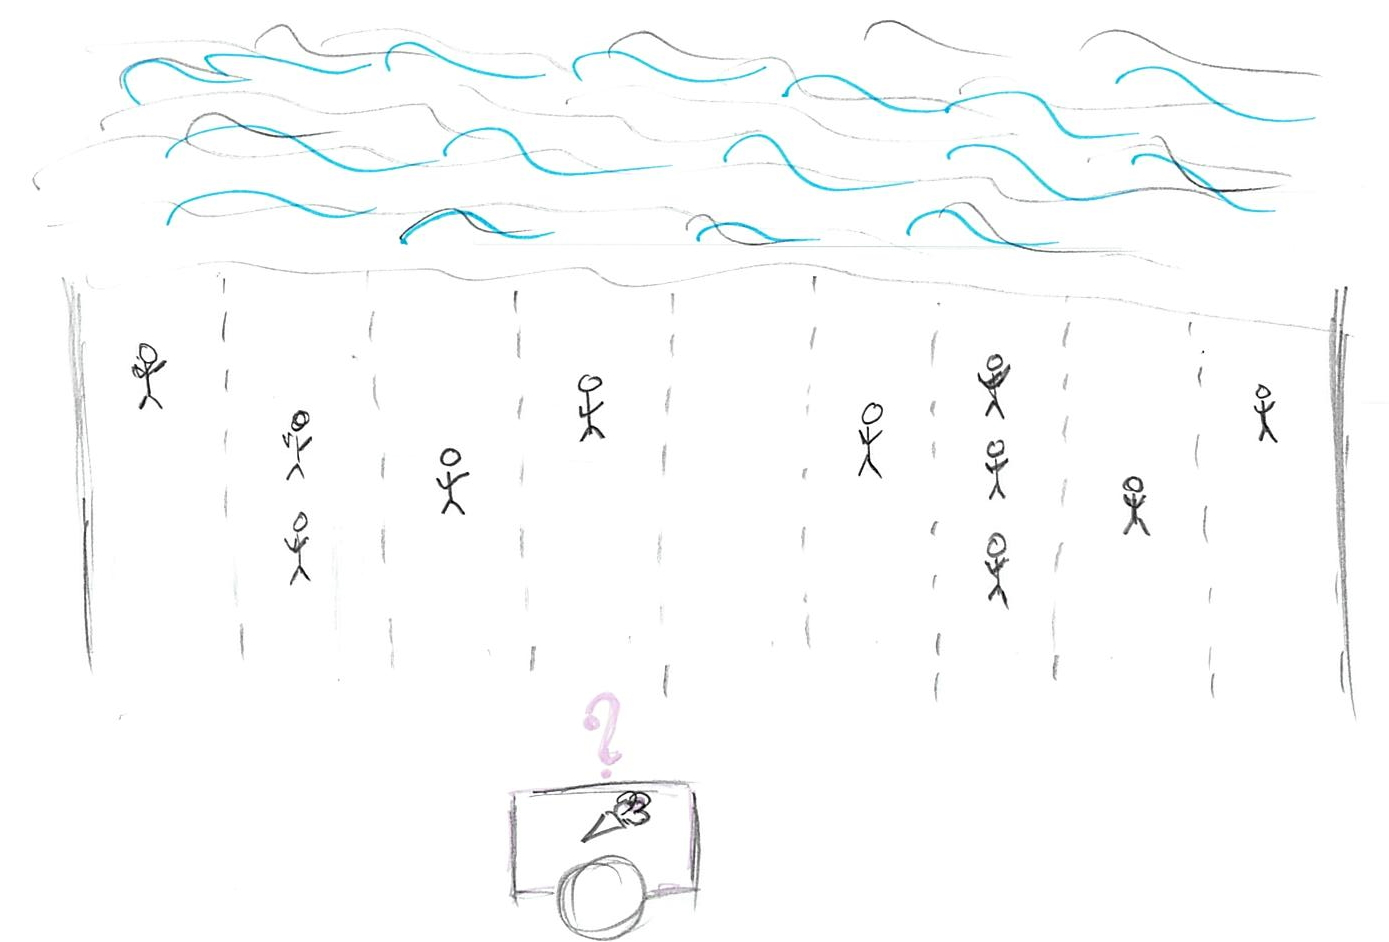
\includegraphics[width=1\linewidth]{images/loss-functions-where-to} \end{center}

\hypertarget{l0-mode}{%
\section{L0 (mode)}\label{l0-mode}}

The simplest loss function is\\
\[L0(stand, person_i) =  \begin{cases}
0, stand == person_i \\
\infty, stand \neq person_i
\end{cases}\]

This function assumes that everybody hates walking so much, that \emph{any} walk is unbearable and should be avoided. Thus, there is no cost for getting your ice-cream only for people who are positioned right next to your stand. For everybody else, even one meter away, the costs of walking are infinite, so they won't bother and, therefore, won't buy your ice-cream. Still, we are in the business of selling one, so where do we put our stand given how lazy our customers are? Well, we just find the biggest group of people and put our stand next to them. No one else will come but at least you got the biggest group of customers you could. If you look at the \emph{distribution} of your customers along the beach this is the highest peak (that you peak) and it is called the \emph{mode} of the distribution.

\begin{center}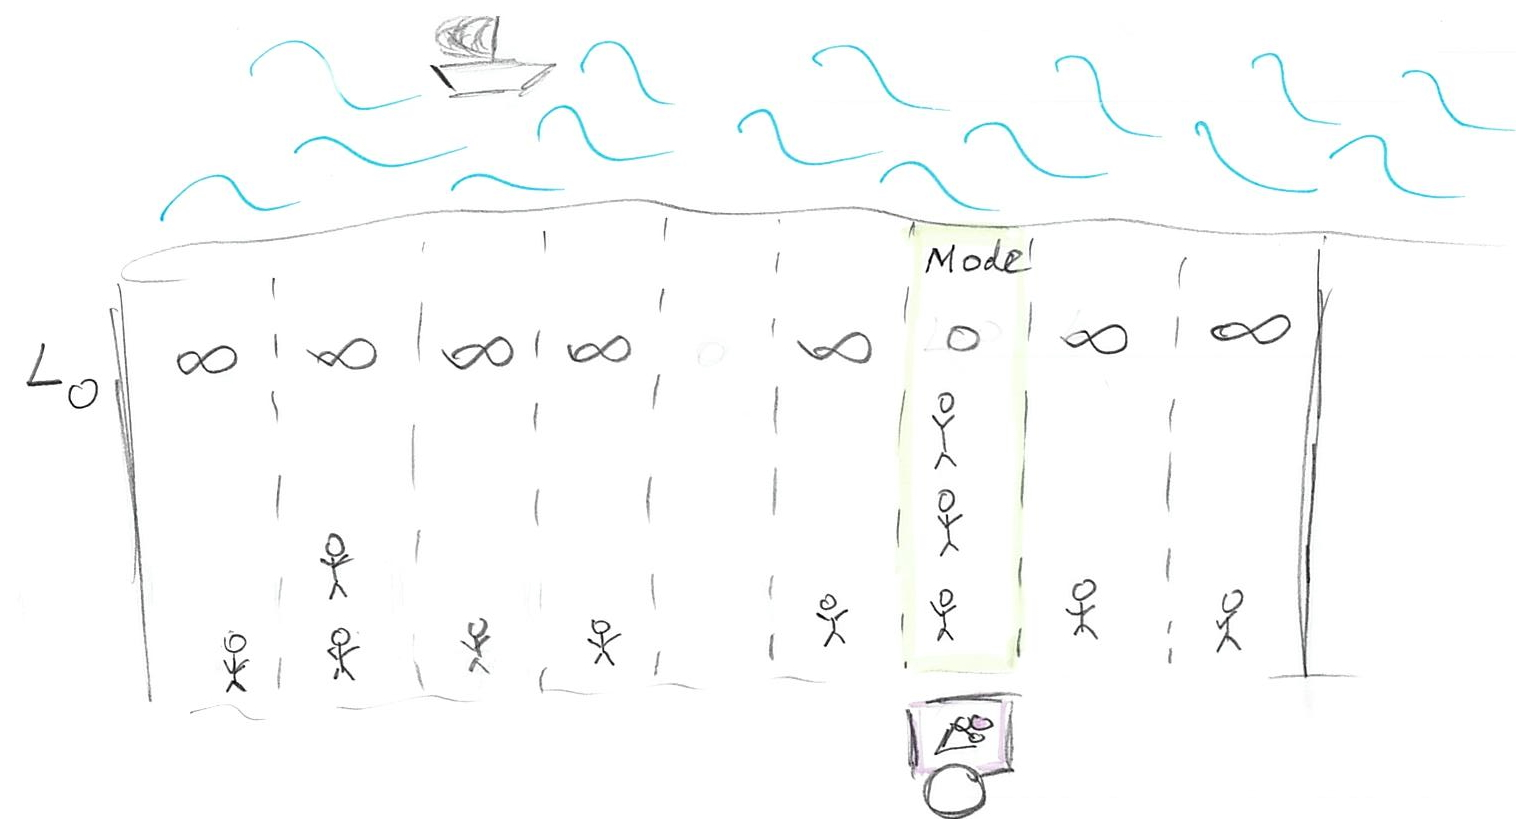
\includegraphics[width=1\linewidth]{images/loss-functions-L0} \end{center}

\hypertarget{l1-median}{%
\section{L1 (median)}\label{l1-median}}

The next loss function, that I already mentioned, assumes a simple linear relationship between the distance and the cost
\[L1(stand, person_i) = |person_i - stand|\]
In other words, the cost is equal to distance (we need \texttt{\textbar{}\ \textbar{}} to get an absolute value, because the person could be ``to the left of'' of stand, in which case \texttt{person\ -\ stand} distance will be negative). So, where should we put our stand? Let us start at a fairly random location so that 3 of our customers are on the left and 7 are on the right.

\begin{center}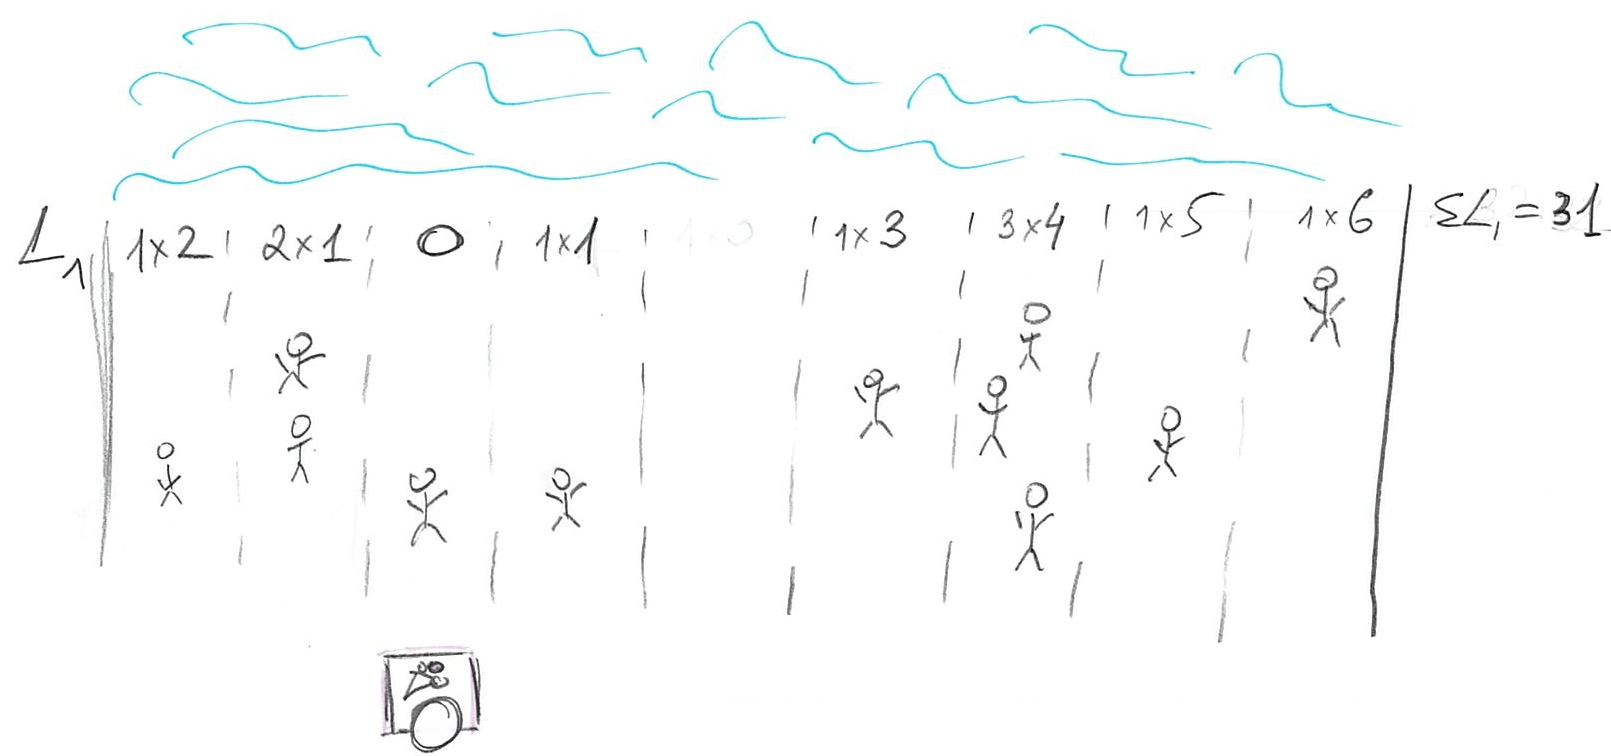
\includegraphics[width=1\linewidth]{images/loss-functions-L1-off-median} \end{center}

We can, in principle, compute the actual cost but it is simpler to ask the question of whether we can \emph{improve} on that cost by moving somewhere else? Imagine that we move to the left where \emph{minority} of our customers are. Now we have 1 on the left and 8 on the right (plus 2 more at our location).

\begin{center}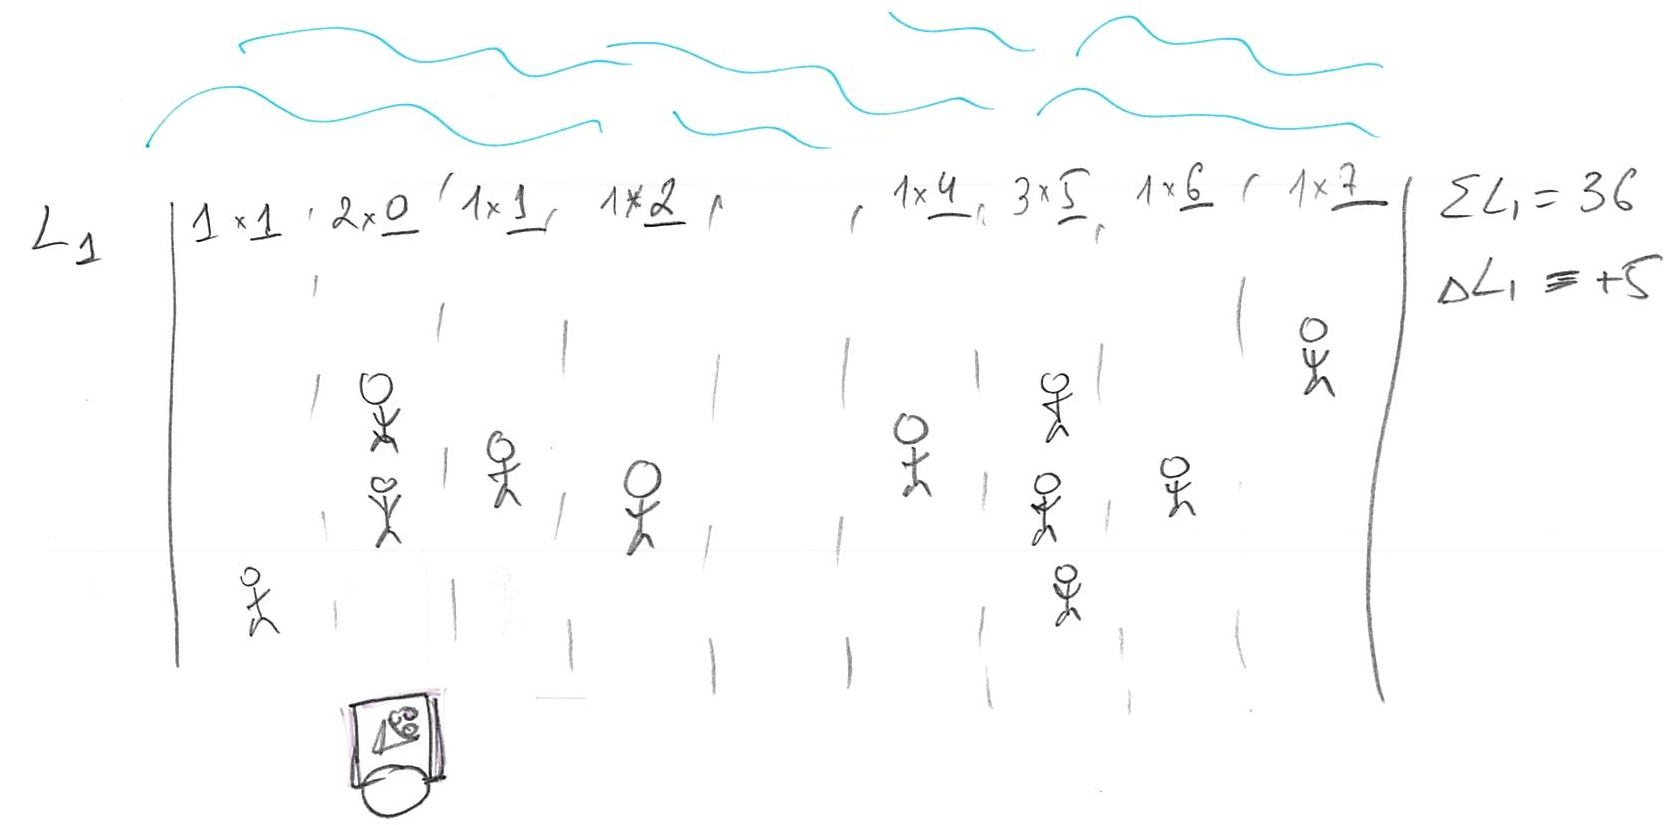
\includegraphics[width=1\linewidth]{images/loss-functions-L1-left} \end{center}

The problem is, we moved \emph{away} from the majority of the people so our total cost is \emph{original cost - 3 (improvement due to moving close to minority) + 8 (increase in loss due to moving away from majority)}, so \(\Delta L1 = +5\). Oops, we made it worse! How about moving to the \emph{right}?

\begin{center}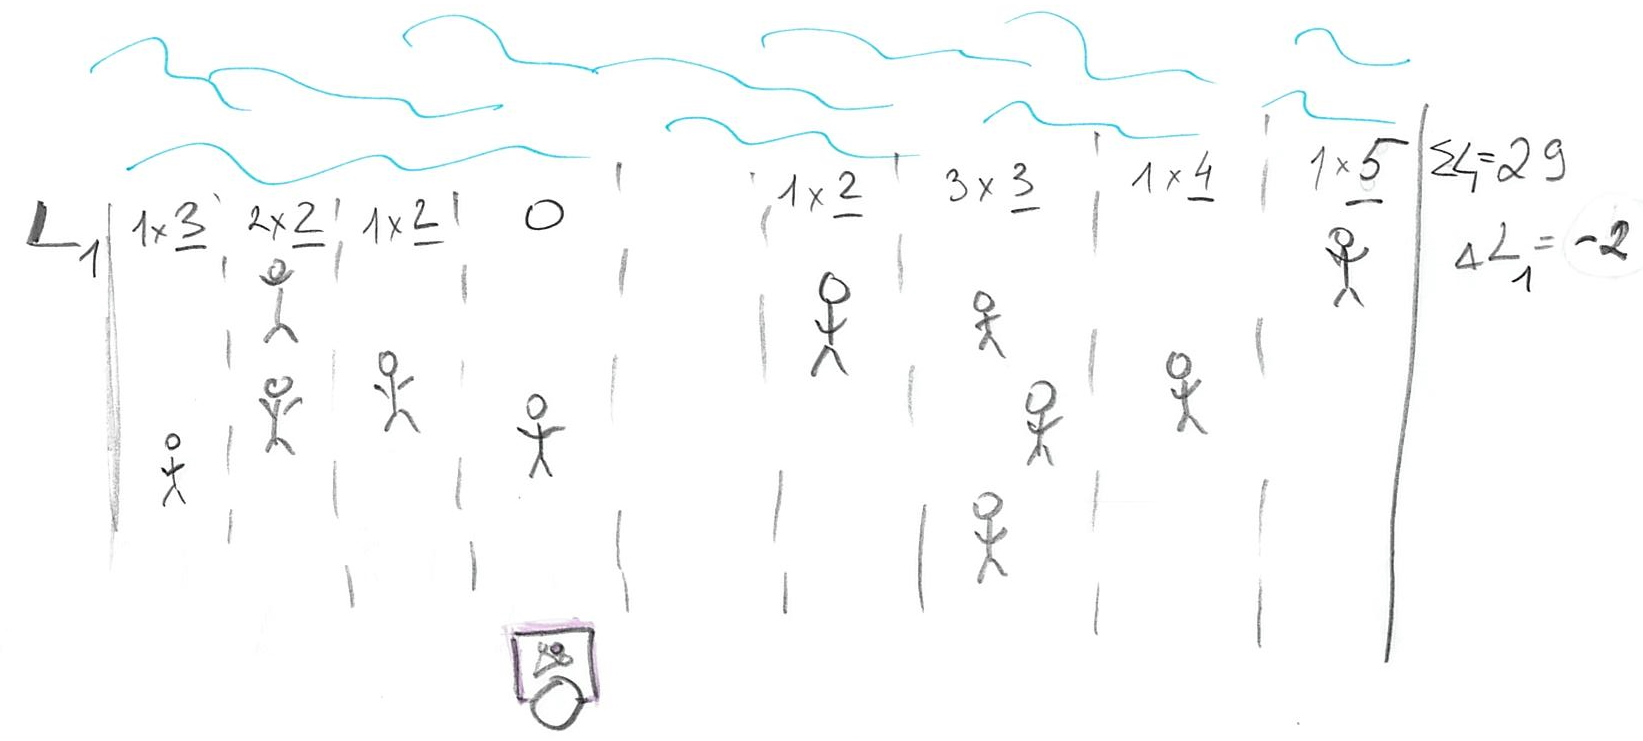
\includegraphics[width=1\linewidth]{images/loss-functions-L1-right} \end{center}

Now that we move \emph{towards} the majority of customers, we have four on the left and six on the right (plus one at our location). The change in cost is \emph{original cost + 4 (loss due to moving away from minority) - 6 (improvement due to moving towards majority)}, so \(\Delta L1 = -2\). Which gives us an idea: we should try to get even closer to that majority by keeping walking to the right! Eventually, you will get to point of the 50/50. Should you keep moving to the right? Should you move to the left? Should you move at all?

\begin{center}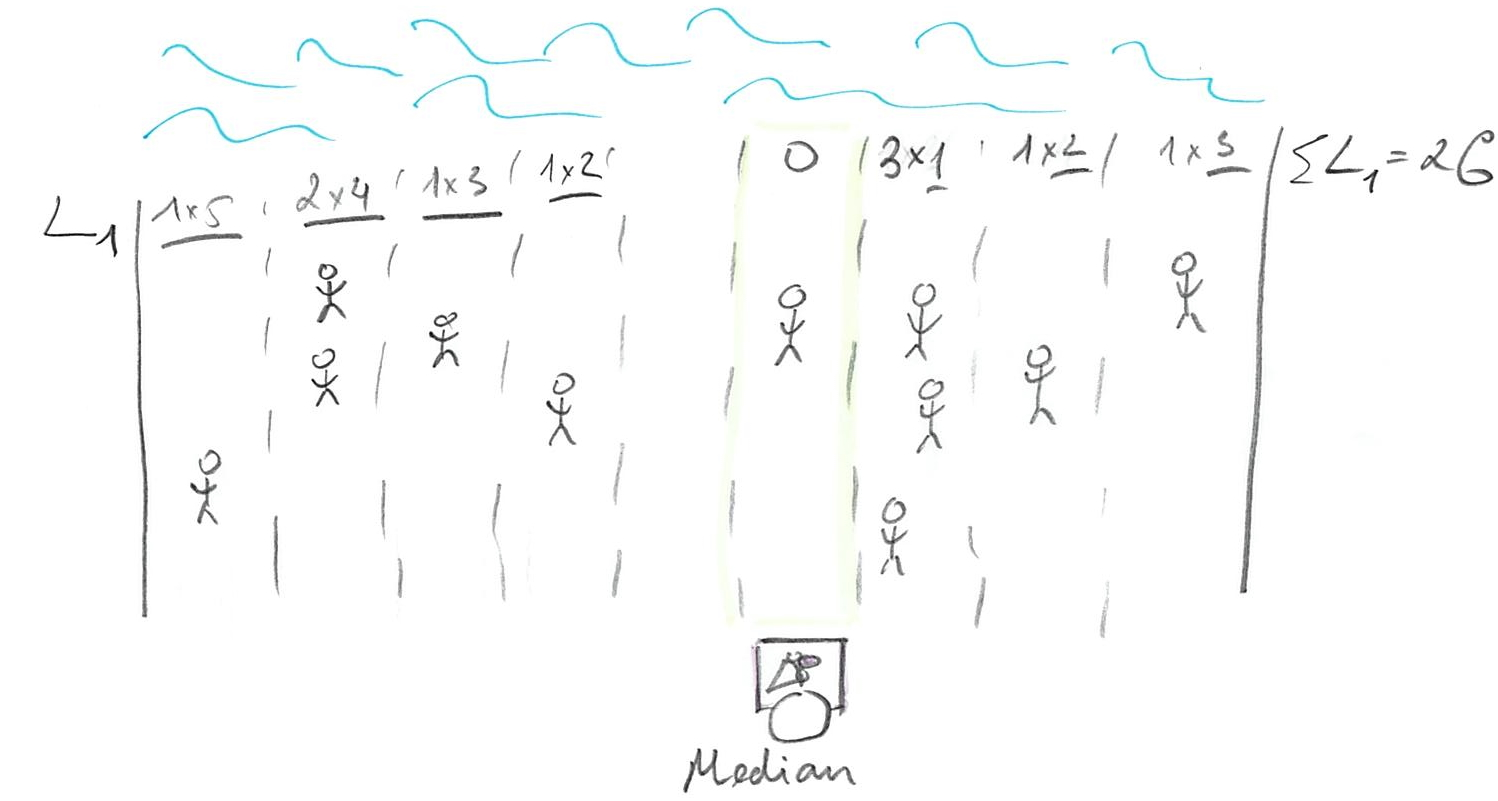
\includegraphics[width=1\linewidth]{images/loss-functions-L1-median} \end{center}

There is no point in moving to the left. You just came from where because moving to the right made things better. However, if you keep moving to the right, you will keep passing people, so that majority now will be on the left and you would be walking \emph{away} from the majority, raising the costs (and your losses). So, once you get to point where half of your customers are on the left and half are on the right, you cannot do any better. Any movement that gets you from 50/50 means there are more customers on one side (say left, if you moved to the right) and, as we already figured out, your best strategy is to move towards the majority, which gets you back where you started at 50/50 point. That 50/50 points split, when half of customers / probability mass is on one side and half is on the other, is called \emph{median}.

\hypertarget{l2-mean}{%
\section{L2 (mean)}\label{l2-mean}}

The classic loss function is Euclidean distance \[L2(stand, person_i) = (person - stand)^2\]
Here, every next step becomes progressively harder for our customers. The cost of walking 1 meter is 1 (unit of effort). But walking 2 is \(2^2 = 4\) and is \(3^2=9\) for 3 meters. Thus, the penalty (cost/loss) for being further away from your stand increases as a power law. Still, one needs to sell ice-cream, so one needs to find the best spot where total cost is minimal

\[L2(stand, person) = \sum_{i=1}^{N}{(person_i - stand)^2}\]

\begin{center}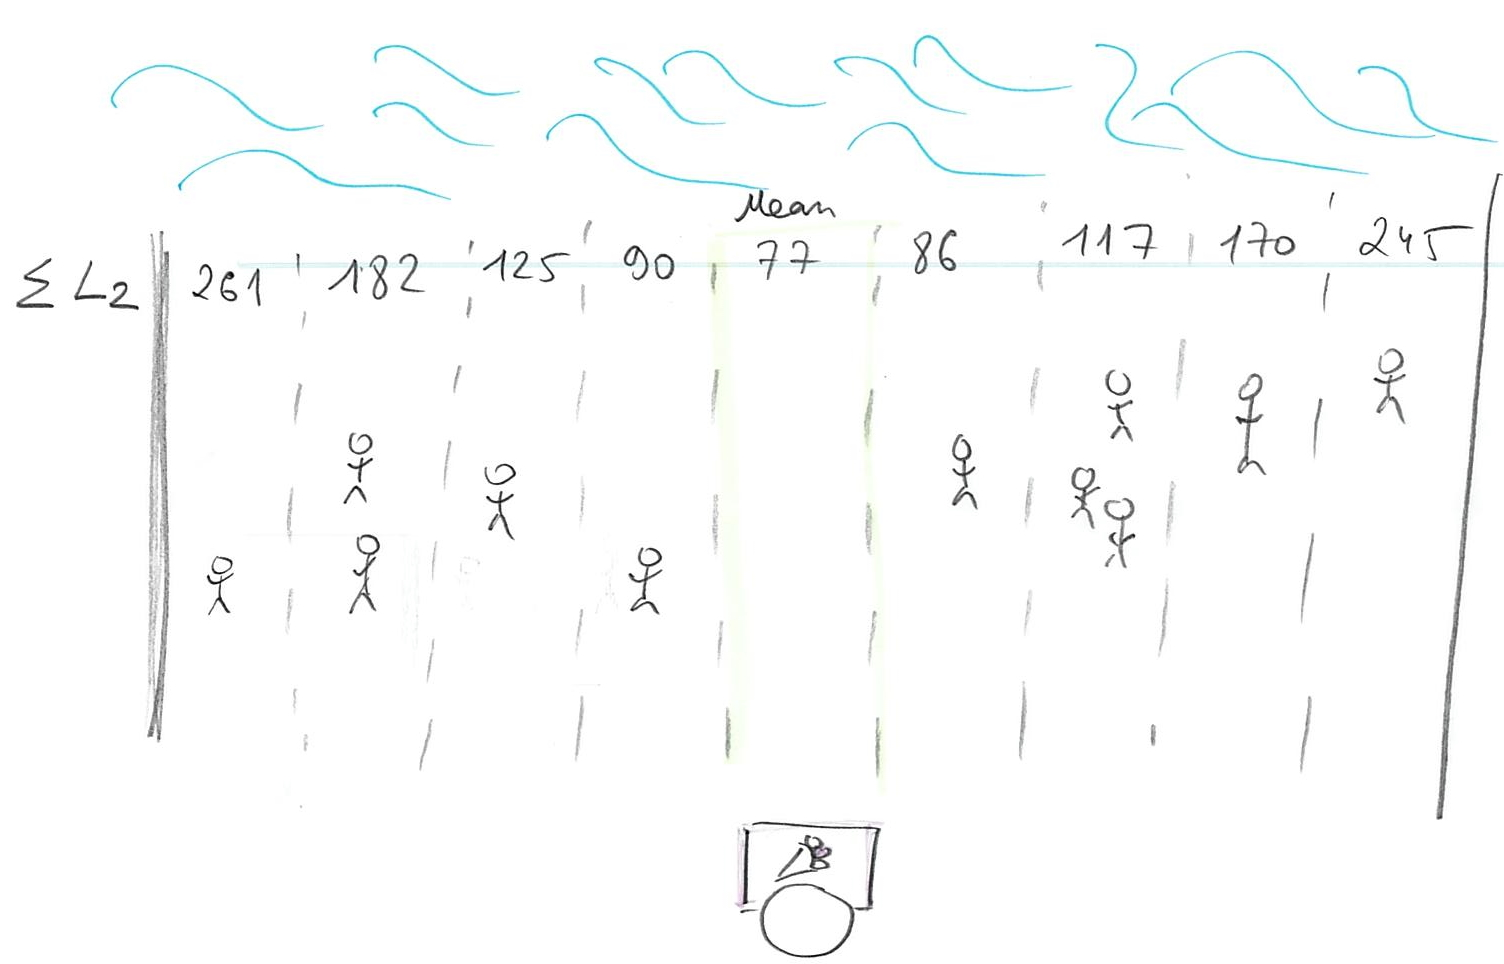
\includegraphics[width=1\linewidth]{images/loss-functions-L2-mean} \end{center}

Or, we can compute the minimal \emph{average} cost by dividing the sum by the total number of customers \texttt{N}:
\[<L2(stand, person)> = \frac{1}{N}\sum_{i=1}^{N}{(person_i - stand)^2}\]

Conceptually, you find that minimum by walking along the beach in the direction that reduces the cost until you hit the point where it start going up again. This strategy is called \emph{gradient descent} and, generally speaking, this is how computer finds minima computationally: They make steps in different directions to see which way is down and keep going until things start going up. However, in one-dimensional well-behaving case we have here things are even simpler as you can use calculus to figure out the solution analytically. If you watched the videos I advertised above, you'll know that the \emph{derivative} of the function is zero at the extrema (minima or maxima), so we just need to differentiate our average \emph{L2} over position of the stand and find where it is zero\footnote{I've nicked the derivations from {[}\url{https://stats.stackexchange.com/a/312997}{]}}.

\[\frac{\partial L2}{\partial stand} = -\frac{2}{N}\sum_{i=1}^{N}{(person_i - stand)}\]
As we want
\[\frac{\partial L2}{\partial stand} = 0\]
we state
\[\frac{2}{N}\sum_{i=1}^{N}{(person_i - stand)} = 0.\]

Opening up brackets and rearranging we get

\[- \frac{2}{N}\sum_{i=1}^{N}{person_i} + \frac{2 \cdot N}{N} \cdot stand = 0 \\
2 \cdot stand = \frac{2}{N}\sum_{i=1}^{N}{person_i} \\
stand = \frac{1}{N}\sum_{i=1}^{N}{person_i}\]

So, the optimal location of your stand is the \emph{mean}: an average location of all people on the beach.

\hypertarget{l1-median-vs.-l2-mean}{%
\section{L1 (median) vs.~L2 (mean)}\label{l1-median-vs.-l2-mean}}

One problem about the \emph{mean} is that it is sensitive to outliers. Because the costs grow as a power law, this approach favors a lot of medium-sized distances over lots of smalls ones plus one really large one. Thus, a single person at a far side of the beach would have a big influence on your stand's location (you already saw the difference in the example above). In data analysis, this means that those outliers will pull your estimates away from the majority of responses. Which is why it might be a good idea to consider using \texttt{median} rather than \texttt{mean}. If you distribution is symmetric, the difference will be negligible but in presence of outliers \texttt{median}, as a point-estimate, is more robust.

\hypertarget{choosing-a-likelihood}{%
\section{Choosing a likelihood}\label{choosing-a-likelihood}}

So far we talked about selling ice-cream on the beach but same question of choosing your loss function applies when you are trying to fit a distribution or a regression line, as in chapter 4. Here, you also have a point-estimate (regression line at each point) and you try to put it in such a way as to minimize the costs of having data points off that line (the distance from the point-estimate of the line and each data point is called a \emph{residual}). The classic way is to use \emph{L2} distance and the approach is called \emph{ordinary least squares}, as you try to minimize squared residuals.

Alternatively, you can express same costs-of-being-off-the-line using a distribution, such as Gaussian. You put its peak (mean) at the (candidate) location of your point estimate (that point has highest probability, so lowest cost) and the loss is computed as a probability of the residual (distance-to-the-point). You can think about it in terms of the probability that a person will go and buy ice-cream from your stand.

\begin{center}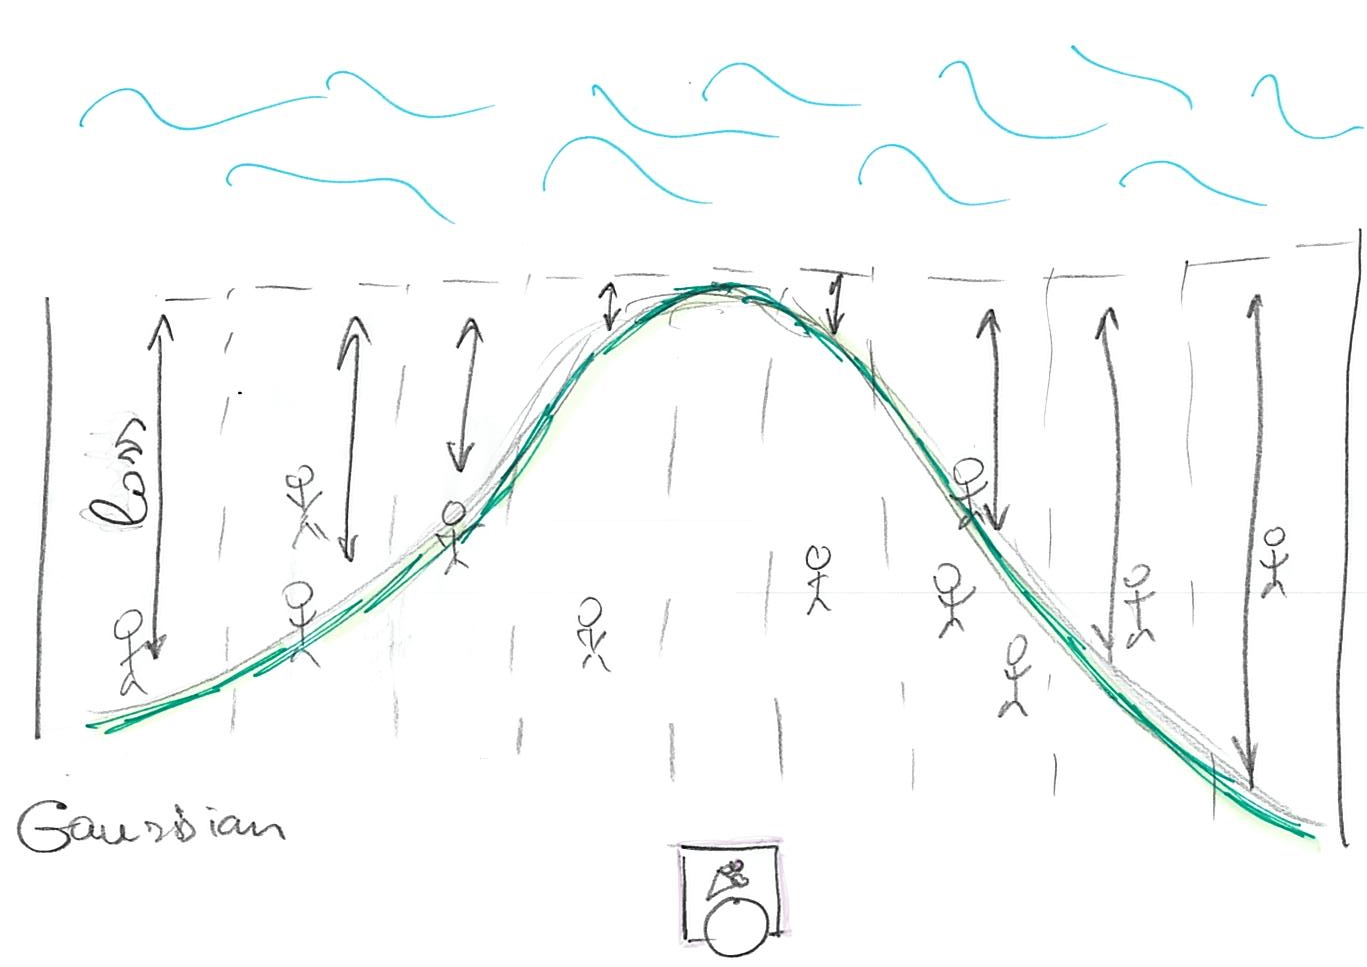
\includegraphics[width=1\linewidth]{images/loss-functions-Gaussian} \end{center}

The Gaussian is special because it uses L2 distance, see \((x - \mu)^2\) inside the exponential:
\[f(x) = \frac{1}{\sigma \sqrt(2 \pi)}e^{\left(-\frac{1}{2}\frac{(x - \mu)^2}{\sigma^2}\right)}\]

so using it is equivalent to fitting via ordinary least squares. However, as McElreath hinted, you can choose different priors that are different not only in the distance-to-loss formula (like \emph{L1} is different from \emph{L2}) but also in symmetry. Both \emph{L1} and \emph{L2} (and Gaussian) ignore the sign of the distance. It does not matter whether customers are on the left or on the right. Other distributions, such as Beta, Gamma, or Log Normal are not symmetric, so the same distance will cost differently depending on the side the customer is at.

\begin{center}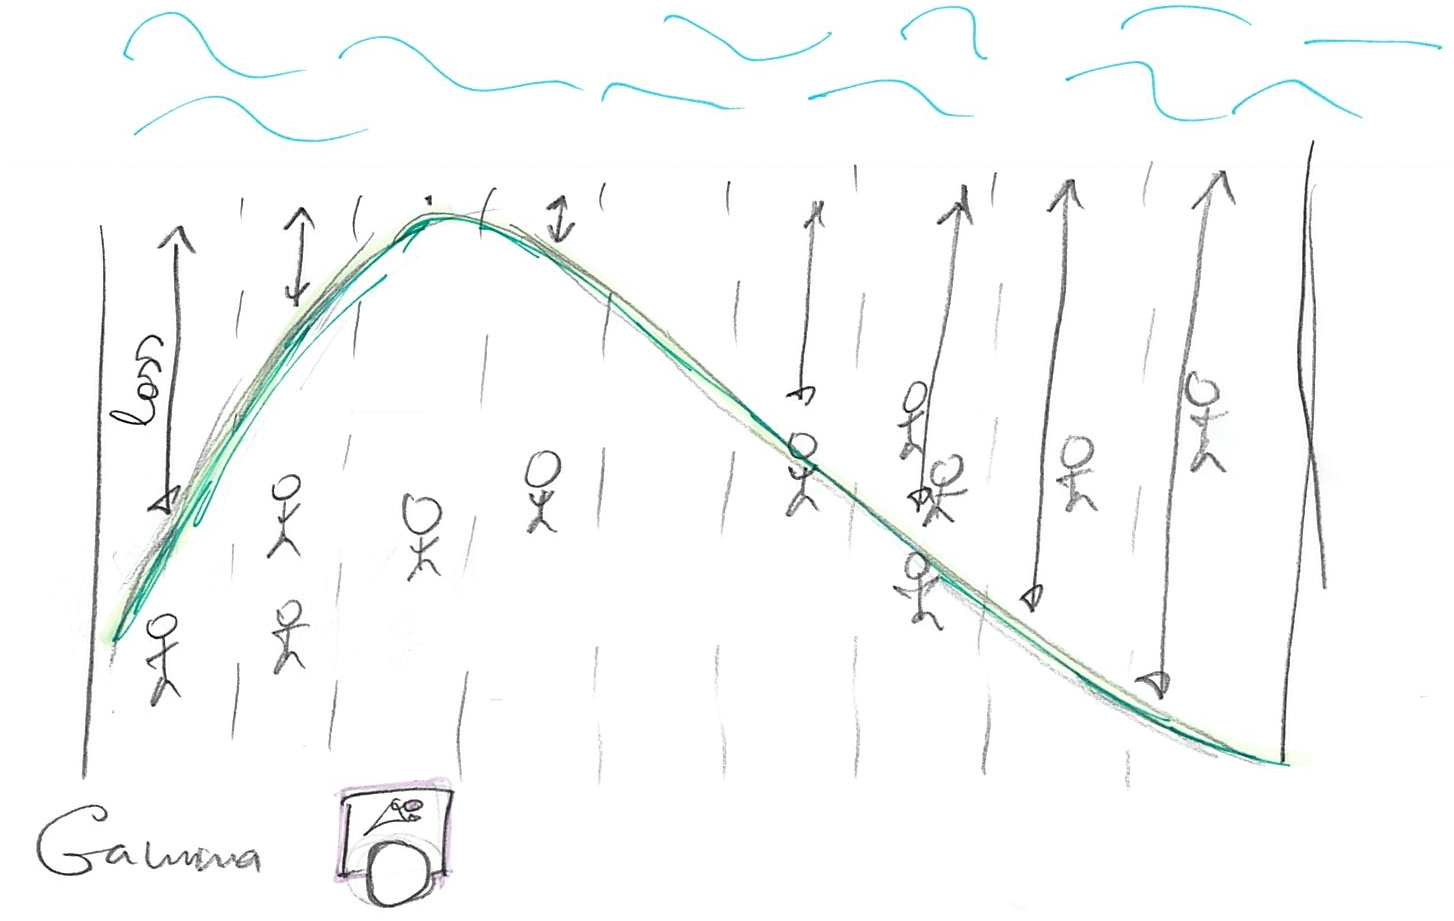
\includegraphics[width=1\linewidth]{images/loss-functions-Gamma} \end{center}

This allows you to think about the choice of your likelihood distribution in terms of choosing a loss function. Both describe how tolerant you are for points to be off the point estimate (regression line). For example, a t-distribution has heavier tails than a Gaussian (if you want to sound like a real mathematician, you say ``leptokurtic''), so its losses for outliers (penalty for larger residuals) are lower. Using it instead of a Gaussian would be similar to changing the loss function from L2 to be more like L1 (e.g.~\(|person_i - stand|^{1.5}\)). Conversely, you can pick a symmetric distribution that is narrower than a Gaussian to make residuals penalty even higher (e.g.~using \((person_i - stand)^{4}\)). You can also consider other properties: Should it be symmetric? Should it operate only within certain range (1..7 for a Likert scale, 0..1 for proportions, positive values for Gamma)? Should it weight all points equally? As you saw in the examples above, picking a different function moves your cart (regression line), so you should keep in mind that using a different likelihood will move the regression line and produce different estimates and predictions.

How do you pick a likelihood/loss function? It depends on the kind of data you have, on your knowledge about the process that generated the data, robustness of inferences in the presence of outliers, etc. However, most real-life cases you are likely to encounter will be covered by the distributions described in the book (Gaussian, exponential, binomial, Poisson, Gamma, etc.). After finishing the book, you will have a basic understanding of which are most appropiate in typical cases. The atypical cases you'll have to research yourself!

\hypertarget{gaussian-in-frenquentist-versus-bayesian-statistics}{%
\section{Gaussian in frenquentist versus Bayesian statistics}\label{gaussian-in-frenquentist-versus-bayesian-statistics}}

Later on in the book McElreath will note that erroneously assuming normal distribution for residuals ruins your inferences in frequentist statistics but not in Bayesian. This is because picking a distribution means different things in frequentist and Bayesian. As I wrote above, in the Bayesian case, likelihood is merely a loss function that translate distance from a data point to a regression line (residual) into a penalty (again, it determines just how tolerant you are for points off the line). Thus, you are using penalties for \emph{observed residuals} and having a bad loss function will make your posterior distribution suboptimal but you still can make inferences because it still is based on your actual residuals.

In contrast, in frequentist statistics, when you are stating that your observed residuals are a sample from a particular distribution, your actual residuals are used to determine parameters of this distribution. Then, however, you make your inferences using \emph{that distribution} not the residuals themselves. This is a very strong conjecture and probably the biggest leap of faith in frequentist statistics saying ``I know the true distribution''. Problem is, if you got your likelihood function / distribution wrong, your inferences are based on a model that describes \emph{something else} not your data. For example, you have a proportion data but you assume Gaussian distribution for residuals and build a model as if your residuals are always symmetrically distributed (not squashed on one side by floor or celing). That model will not be about your data, it will be about normally distributed \emph{something else}. The numbers for that \emph{something else} may look good (or bad) but they are not the numbers you are interested in. This is a mistake that is remarkably easy to do because computers won't stop you from making it. Think back to Chapter 1: Golems don't care! You can abuse any statistical model/test and they will simply spit out the numbers, even if tests are completely unsuitable for your data. Making sure that distribution is correct and that you are doing the right thing is on you, not the Golem!

\hypertarget{solutions-for-chapter-2}{%
\chapter{Solutions for Chapter 2}\label{solutions-for-chapter-2}}

\begin{Shaded}
\begin{Highlighting}[]
\KeywordTok{library}\NormalTok{(tidyverse)}
\KeywordTok{library}\NormalTok{(rethinking)}
\end{Highlighting}
\end{Shaded}

\hypertarget{e1}{%
\subsubsection*{2E1}\label{e1}}
\addcontentsline{toc}{subsubsection}{2E1}

Which of the expressions below correspond to the statement: the probability of rain on Monday?

\begin{enumerate}
\def\labelenumi{\arabic{enumi}.}
\tightlist
\item
  Pr(rain)
\item
  \textbf{Pr(rain \textbar{} Monday) ✓}
\item
  Pr(Monday \textbar{} rain)
\item
  Pr(rain, Monday) / Pr(Monday)
\end{enumerate}

\hypertarget{e2}{%
\subsubsection*{2E2}\label{e2}}
\addcontentsline{toc}{subsubsection}{2E2}

Which of the following statements corresponds to the expression: Pr(Monday\textbar rain)?

\begin{enumerate}
\def\labelenumi{\arabic{enumi}.}
\tightlist
\item
  The probability of rain on Monday.
\item
  The probability of rain, given that it is Monday.
\item
  \textbf{The probability that it is Monday, given that it is raining. ✓}
\item
  The probability that it is Monday and that it is raining.
\end{enumerate}

\hypertarget{e3}{%
\subsubsection*{2E3}\label{e3}}
\addcontentsline{toc}{subsubsection}{2E3}

Which of the expressions below correspond to the statement: the probability that it is Monday, given that it is raining?

\begin{enumerate}
\def\labelenumi{\arabic{enumi}.}
\tightlist
\item
  \textbf{Pr ( Monday \textbar{} rain ) ✓}
\item
  Pr(rain \textbar{} Monday)
\item
  Pr(rain \textbar{} Monday) Pr(Monday)
\item
  \textbf{Pr(rain \textbar{} Monday) Pr(Monday) / Pr(rain)✓}
\item
  Pr(Monday \textbar{} rain) Pr(rain) / Pr(Monday)
\end{enumerate}

\hypertarget{e4}{%
\subsubsection*{2E4}\label{e4}}
\addcontentsline{toc}{subsubsection}{2E4}

The Bayesian statistician Bruno de Finetti (1906-- 1985) began his 1973 book on probability theory with the declaration: ``PROBABILITY DOES NOT EXIST.'' The capitals appeared in the original, so I imagine de Finetti wanted us to shout this statement. What he meant is that probability is a device for describing uncertainty from the perspective of an observer with limited knowledge; it has no objective reality. Discuss the globe tossing example from the chapter, in light of this statement. What does it mean to say ``the probability of water is 0.7''?

\begin{center}\rule{0.5\linewidth}{0.5pt}\end{center}

He meant that, at least at macro level, there are no truly random events. At that scale, all events, such as motion of a globe throughout its flight, are described by deterministic laws of physics. Therefore, the outcome of globe tossing is deterministic and predictable if we have a complete knowledge about its initial momentum and about other forces at play (e.g., air movement). In most cases, we do not have the full knowledge and, therefore, our predictions are likely to diverge from the observed outcome and be mostly but not always correct. Hence, the concept of probability. At the end, noise is never truly random, noise is information that we did not include into our model explicitly.

\hypertarget{m1}{%
\subsubsection*{2M1}\label{m1}}
\addcontentsline{toc}{subsubsection}{2M1}

Recall the globe tossing model from the chapter. Compute and plot the grid approximate posterior distribution for each of the following sets of observations. In each case, assume a uniform prior for p.

\begin{Shaded}
\begin{Highlighting}[]
\CommentTok{\#\textquotesingle{} Computes posterior for water probability assuming binomial likelihood}
\CommentTok{\#\textquotesingle{}}
\CommentTok{\#\textquotesingle{} @param observations vector of "W" and "L"}
\CommentTok{\#\textquotesingle{} @param prior numeric vector, its length determines grid resolution}
\CommentTok{\#\textquotesingle{}}
\CommentTok{\#\textquotesingle{} @return tibble with Pwater (from 0 to 1), Posterior (probability of water for given Pwater), and Prior}
\CommentTok{\#\textquotesingle{}}
\CommentTok{\#\textquotesingle{} @examples}
\CommentTok{\#\textquotesingle{} probability\_of\_water(c("W", "W", "W"), rep(1, 100))}
\NormalTok{probability\_of\_water \textless{}{-}}\StringTok{ }\ControlFlowTok{function}\NormalTok{(observations, prior)\{}
\NormalTok{  p\_grid \textless{}{-}}\StringTok{ }\KeywordTok{seq}\NormalTok{(}\DataTypeTok{from=}\DecValTok{0}\NormalTok{, }\DataTypeTok{to=}\DecValTok{1}\NormalTok{, }\DataTypeTok{length.out=}\KeywordTok{length}\NormalTok{(prior))}
\NormalTok{  likelihood \textless{}{-}}\StringTok{ }\KeywordTok{dbinom}\NormalTok{(}\KeywordTok{sum}\NormalTok{(observations }\OperatorTok{==}\StringTok{ "W"}\NormalTok{), }\DataTypeTok{size=}\KeywordTok{length}\NormalTok{(observations), }\DataTypeTok{prob=}\NormalTok{p\_grid)}
\NormalTok{  unstandardized\_posterior \textless{}{-}}\StringTok{ }\NormalTok{likelihood }\OperatorTok{*}\StringTok{ }\NormalTok{prior}
  \KeywordTok{tibble}\NormalTok{(}\DataTypeTok{Pwater =}\NormalTok{ p\_grid,}
         \DataTypeTok{Posterior =}\NormalTok{ unstandardized\_posterior }\OperatorTok{/}\StringTok{ }\KeywordTok{sum}\NormalTok{(unstandardized\_posterior),}
         \DataTypeTok{Prior =}\NormalTok{ prior)}
\NormalTok{\}}
\end{Highlighting}
\end{Shaded}

\textbf{1. W, W, W}

\begin{Shaded}
\begin{Highlighting}[]
\NormalTok{posterior2M1 \textless{}{-}}\StringTok{ }\KeywordTok{probability\_of\_water}\NormalTok{(}\KeywordTok{c}\NormalTok{(}\StringTok{"W"}\NormalTok{, }\StringTok{"W"}\NormalTok{, }\StringTok{"W"}\NormalTok{), }\KeywordTok{rep}\NormalTok{(}\DecValTok{1}\NormalTok{, }\DecValTok{100}\NormalTok{))}
\KeywordTok{ggplot}\NormalTok{(posterior2M1, }\KeywordTok{aes}\NormalTok{(}\DataTypeTok{x=}\NormalTok{Pwater, }\DataTypeTok{y=}\NormalTok{Posterior)) }\OperatorTok{+}\StringTok{ }
\StringTok{  }\KeywordTok{geom\_line}\NormalTok{()}
\end{Highlighting}
\end{Shaded}

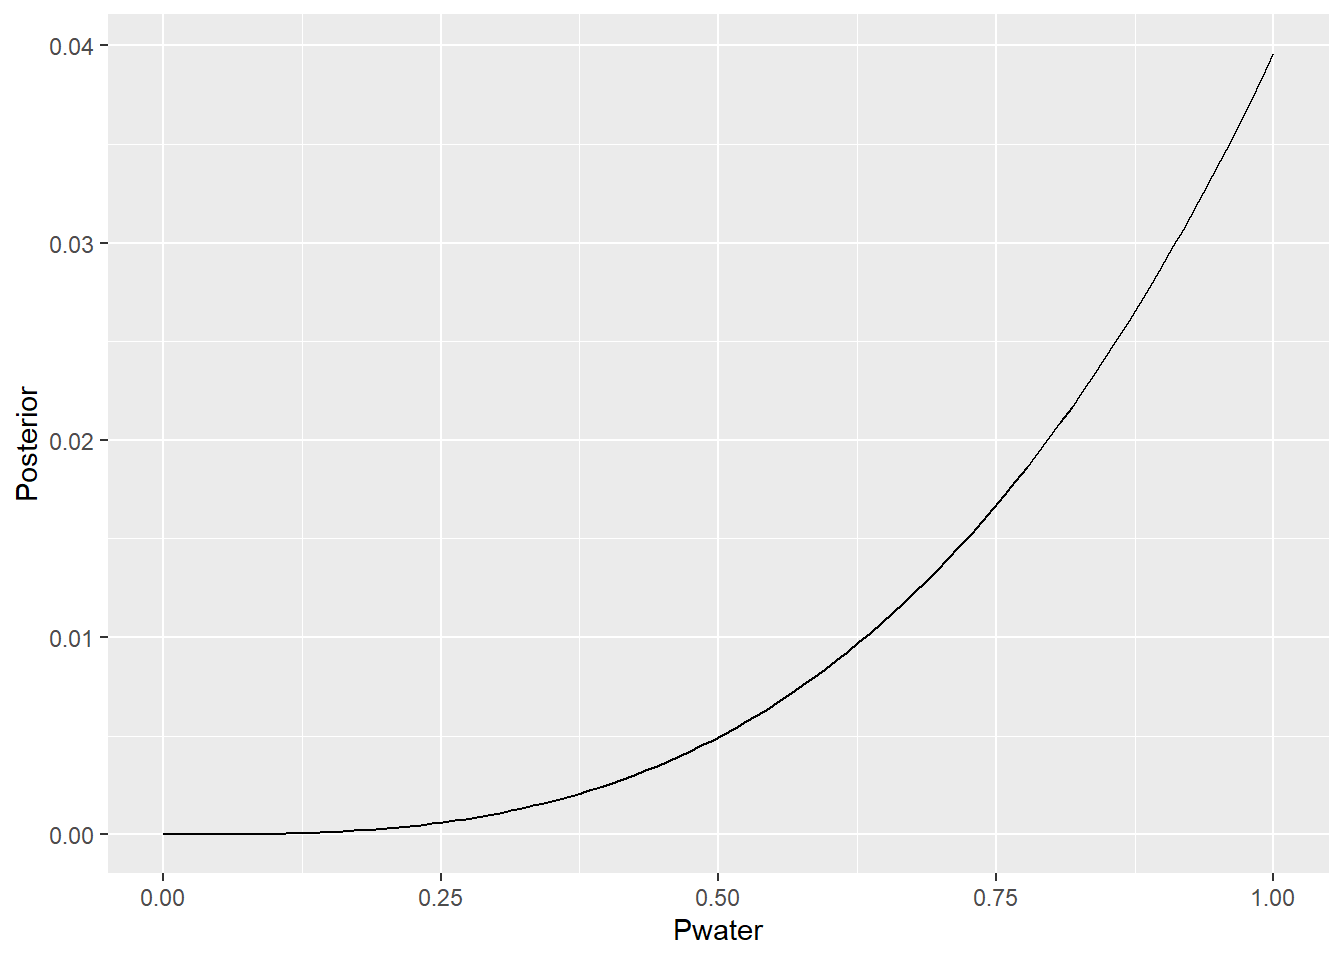
\includegraphics{notes-on-statistical-rethinking_files/figure-latex/2M1-1-1.pdf}

\textbf{2. W, W, W, L}

\begin{Shaded}
\begin{Highlighting}[]
\NormalTok{posterior2M2 \textless{}{-}}\StringTok{ }\KeywordTok{probability\_of\_water}\NormalTok{(}\KeywordTok{c}\NormalTok{(}\StringTok{"W"}\NormalTok{, }\StringTok{"W"}\NormalTok{, }\StringTok{"W"}\NormalTok{, }\StringTok{"L"}\NormalTok{), }\KeywordTok{rep}\NormalTok{(}\DecValTok{1}\NormalTok{, }\DecValTok{100}\NormalTok{))}
\KeywordTok{ggplot}\NormalTok{(posterior2M2, }\KeywordTok{aes}\NormalTok{(}\DataTypeTok{x=}\NormalTok{Pwater, }\DataTypeTok{y=}\NormalTok{Posterior)) }\OperatorTok{+}\StringTok{ }
\StringTok{  }\KeywordTok{geom\_line}\NormalTok{()}
\end{Highlighting}
\end{Shaded}

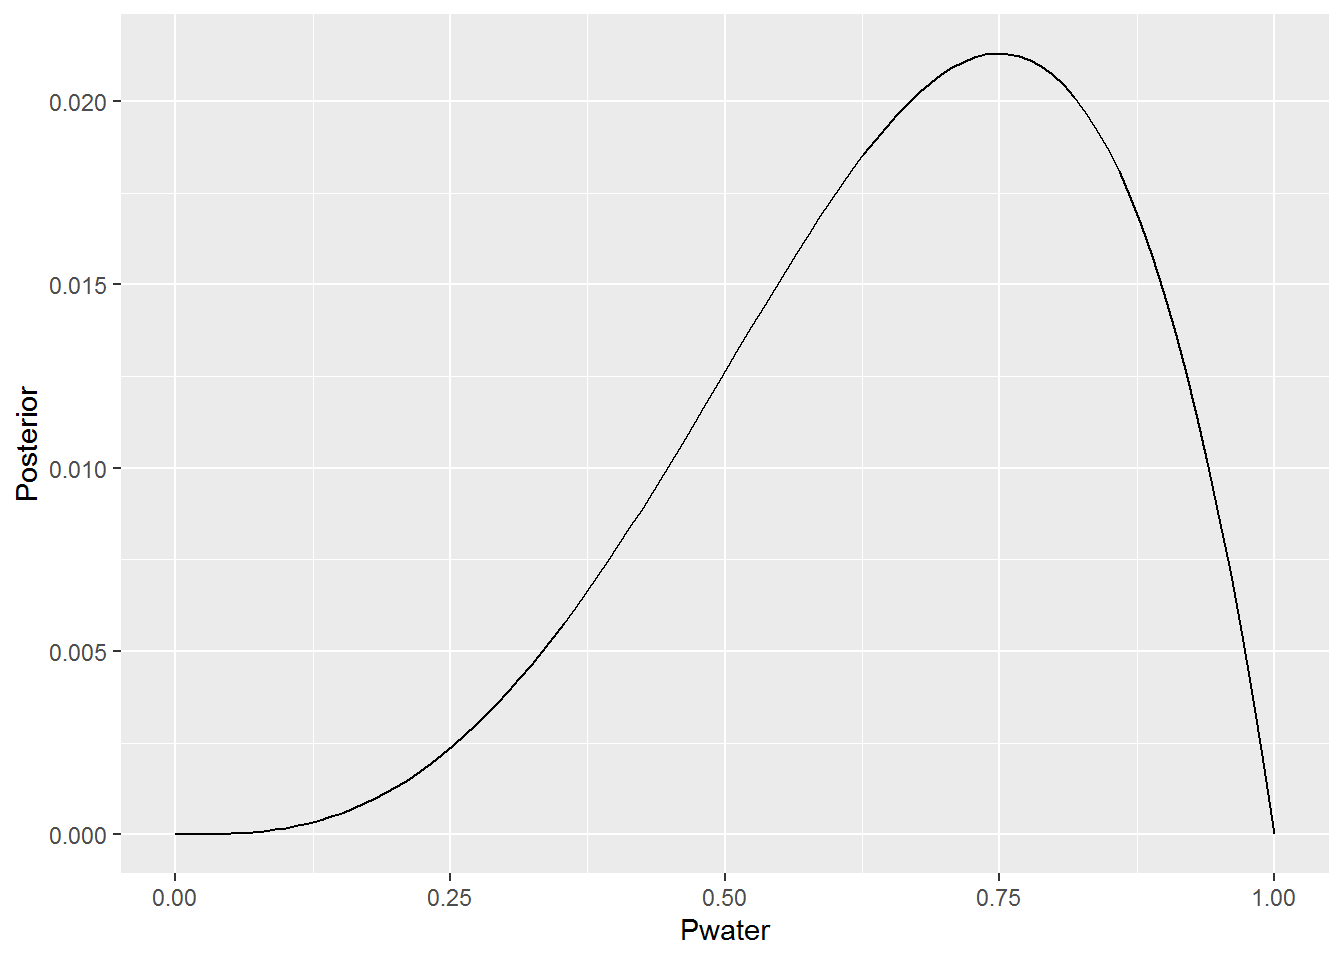
\includegraphics{notes-on-statistical-rethinking_files/figure-latex/2M1-2-1.pdf}

\textbf{3. L, W, W, L, W, W, W}

\begin{Shaded}
\begin{Highlighting}[]
\NormalTok{posterior2M3 \textless{}{-}}\StringTok{ }\KeywordTok{probability\_of\_water}\NormalTok{(}\KeywordTok{c}\NormalTok{(}\StringTok{"L"}\NormalTok{, }\StringTok{"W"}\NormalTok{, }\StringTok{"W"}\NormalTok{, }\StringTok{"L"}\NormalTok{, }\StringTok{"W"}\NormalTok{, }\StringTok{"W"}\NormalTok{, }\StringTok{"W"}\NormalTok{), }\KeywordTok{rep}\NormalTok{(}\DecValTok{1}\NormalTok{, }\DecValTok{100}\NormalTok{))}
\KeywordTok{ggplot}\NormalTok{(posterior2M3, }\KeywordTok{aes}\NormalTok{(}\DataTypeTok{x=}\NormalTok{Pwater, }\DataTypeTok{y=}\NormalTok{Posterior)) }\OperatorTok{+}\StringTok{ }
\StringTok{  }\KeywordTok{geom\_line}\NormalTok{()}
\end{Highlighting}
\end{Shaded}

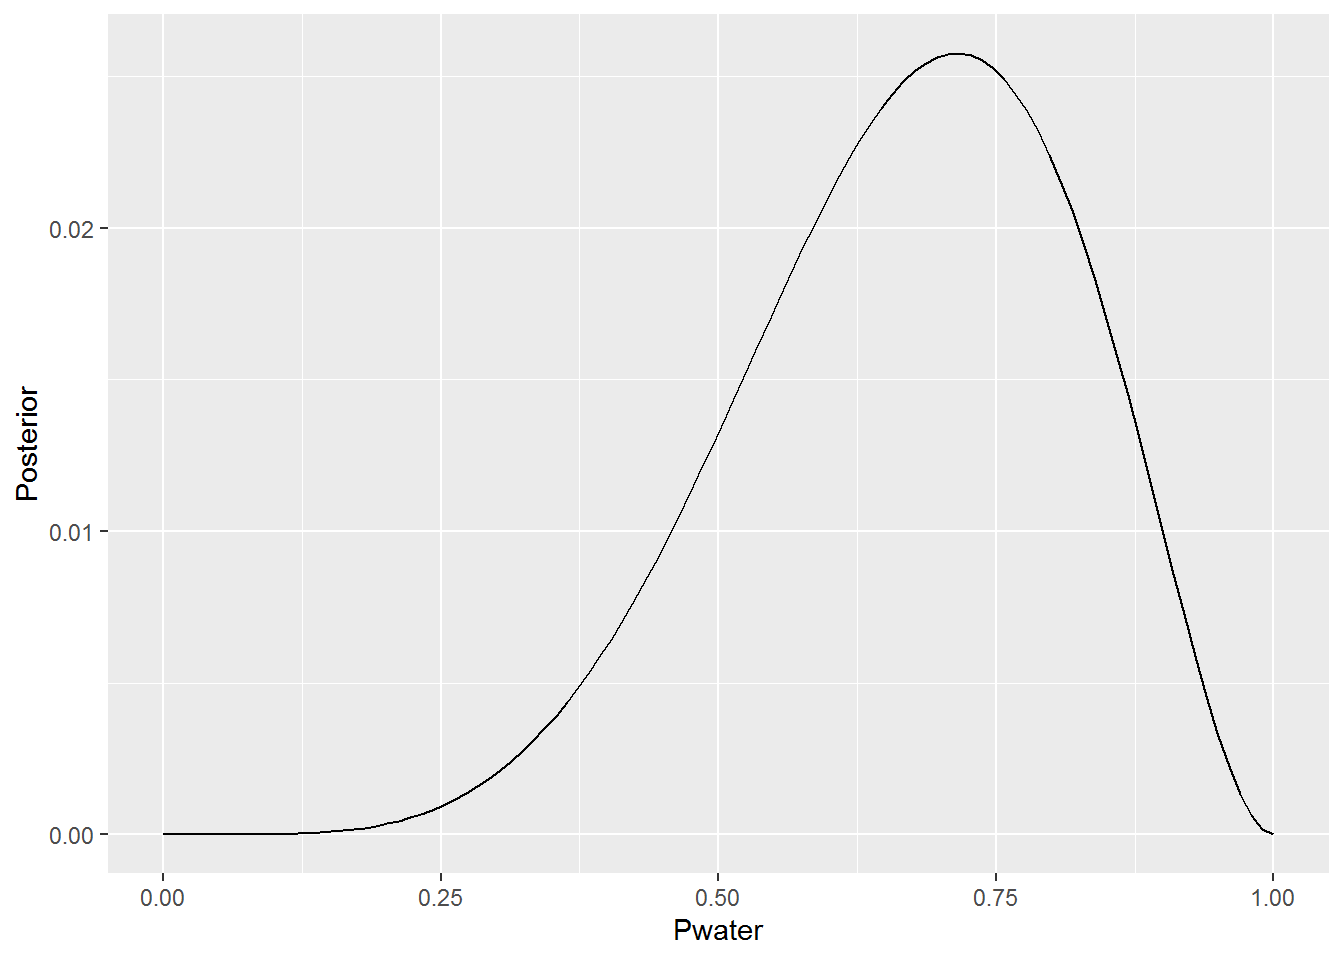
\includegraphics{notes-on-statistical-rethinking_files/figure-latex/2M1-3-1.pdf}

\hypertarget{m2}{%
\subsubsection*{2M2}\label{m2}}
\addcontentsline{toc}{subsubsection}{2M2}

Now assume a prior for p that is equal to zero when p\textless0.5 and is a positive constant when p≥0.5. Again compute and plot the grid approximate posterior distribution for each of the sets of observations in the problem just above.

\begin{Shaded}
\begin{Highlighting}[]
\NormalTok{p\_grid \textless{}{-}}\StringTok{ }\KeywordTok{seq}\NormalTok{(}\DataTypeTok{from=}\DecValTok{0}\NormalTok{, }\DataTypeTok{to=}\DecValTok{1}\NormalTok{, }\DataTypeTok{length.out =} \DecValTok{100}\NormalTok{)}
\NormalTok{priorM2 \textless{}{-}}\StringTok{ }\KeywordTok{as.numeric}\NormalTok{(p\_grid }\OperatorTok{\textgreater{}=}\StringTok{ }\FloatTok{0.5}\NormalTok{)}

\NormalTok{posterior2M3 \textless{}{-}}\StringTok{ }\KeywordTok{probability\_of\_water}\NormalTok{(}\KeywordTok{c}\NormalTok{(}\StringTok{"L"}\NormalTok{, }\StringTok{"W"}\NormalTok{, }\StringTok{"W"}\NormalTok{, }\StringTok{"L"}\NormalTok{, }\StringTok{"W"}\NormalTok{, }\StringTok{"W"}\NormalTok{, }\StringTok{"W"}\NormalTok{), priorM2)}
\KeywordTok{ggplot}\NormalTok{(posterior2M3, }\KeywordTok{aes}\NormalTok{(}\DataTypeTok{x=}\NormalTok{Pwater, }\DataTypeTok{y=}\NormalTok{Posterior)) }\OperatorTok{+}\StringTok{ }
\StringTok{  }\KeywordTok{geom\_line}\NormalTok{() }
\end{Highlighting}
\end{Shaded}

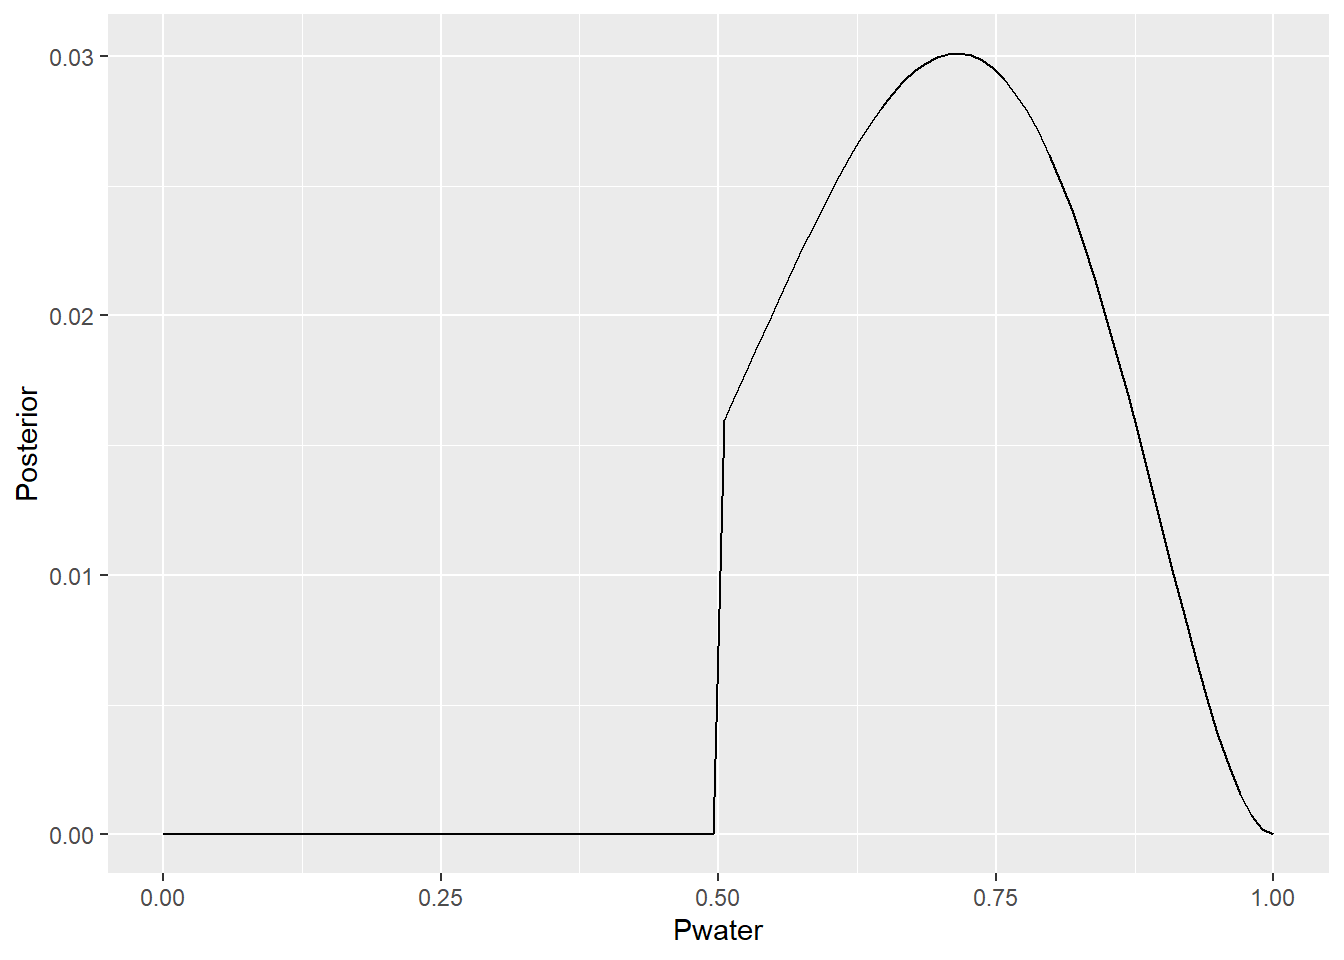
\includegraphics{notes-on-statistical-rethinking_files/figure-latex/2M2-1.pdf}

\hypertarget{m3}{%
\subsubsection*{2M3}\label{m3}}
\addcontentsline{toc}{subsubsection}{2M3}

Suppose there are two globes, one for Earth and one for Mars. The Earth globe is 70\% covered in water. The Mars globe is 100\% land. Further suppose that one of these globes --- you don't know which --- was tossed in the air and produced a ``land'' observation. Assume that each globe was equally likely to be tossed. Show that the posterior probability that the globe was the Earth, conditional on seeing ``land'' (Pr ( Earth \textbar{} land ) ), is 0.23.

\begin{center}\rule{0.5\linewidth}{0.5pt}\end{center}

Bayes Formula tells us that
\[Pr(Planet | land) = \frac{Pr(land | Planet) Pr(Planet)}{Pr(land)}\]
As \(Pr(land)\) is a normalization constant, we can ignore it for a moment. Accordingly,
\[uPr(Earth | land) = 0.3 \cdot 0.5 = 0.15\\
uPr(Mars | land) = 1 \cdot 0.5 = 0.5\]
where \(uPr()\) is unstandardized plausibility. Normalizing it, we get
\[Pr(Earth | land) = \frac{0.15}{0.15 + 0.5} = 0.2308\]

\hypertarget{m4}{%
\subsubsection*{2M4}\label{m4}}
\addcontentsline{toc}{subsubsection}{2M4}

Suppose you have a deck with only three cards. Each card has two sides, and each side is either black or white. One card has two black sides. The second card has one black and one white side. The third card has two white sides. Now suppose all three cards are placed in a bag and shuffled. Someone reaches into the bag and pulls out a card and places it flat on a table. A black side is shown facing up, but you don't know the color of the side facing down. Show that the probability that the other side is also black is 2/3. Use the counting method (Section 2 of the chapter) to approach this problem. This means counting up the ways that each card could produce the observed data (a black side facing up on the table).

\begin{itemize}
\tightlist
\item
  B\textbar B: B(1) → \textbf{B(2) : 1}
\item
  B\textbar B: B(2) → \textbf{B(1) : 1}
\item
  B\textbar W : B → W : 1
\item
  W\textbar B : 0
\item
  W\textbar W : 0
\item
  W\textbar W : 0
\end{itemize}

There are three possible outcomes, given the visible side is black and two out of three lead to a black back side: \(\frac{2}{3}\).

\hypertarget{m5}{%
\subsubsection*{2M5}\label{m5}}
\addcontentsline{toc}{subsubsection}{2M5}

Now suppose there are four cards: B/B, B/W, W/W, and another B/B. Again suppose a card is drawn from the bag and a black side appears face up. Again calculate the probability that the other side is black.

\begin{itemize}
\tightlist
\item
  B\textbar B: B(1) → \textbf{B(2): 1}
\item
  B\textbar B: B(2) → \textbf{B(1) : 1}
\item
  B\textbar W : B → W : 1
\item
  W\textbar B : 0
\item
  W\textbar W : 0
\item
  W\textbar W : 0
\item
  B\textbar B: B(3) → \textbf{B(4): 1}
\item
  B\textbar B: B(4) → \textbf{B(3) : 1}
\end{itemize}

There are three possible outcomes, given the visible side is black and four out of five lead to a black back side: \(\frac{4}{5}\)

\hypertarget{m6}{%
\subsubsection*{2M6}\label{m6}}
\addcontentsline{toc}{subsubsection}{2M6}

Imagine that black ink is heavy, and so cards with black sides are heavier than cards with white sides. As a result, it's less likely that a card with black sides is pulled from the bag. So again assume there are three cards: B/B, B/W, and W/W. After experimenting a number of times, you conclude that for every way to pull the B/B card from the bag, there are 2 ways to pull the B/W card and 3 ways to pull the W/W card. Again suppose that a card is pulled and a black side appears face up. Show that the probability the other side is black is now 0.5. Use the counting method, as before.

\begin{itemize}
\tightlist
\item
  B\textbar B: B(1) → \textbf{B(2): 1 × 1 (prior) = 1}
\item
  B\textbar B: B(2) → \textbf{B(1) : 1 × 1 (prior) = 1}
\item
  B\textbar W : B → W : 1 × 2 (prior) = 2
\item
  W\textbar B : 0 × 2 (prior) = 0
\item
  W\textbar W : 0 × 3 (prior) = 0
\item
  W\textbar W : 0 × 3 (prior) = 0
\end{itemize}

Now the counts are two out of four that other side is black, i.e.~\(0.5\).

\hypertarget{m7}{%
\subsubsection*{2M7}\label{m7}}
\addcontentsline{toc}{subsubsection}{2M7}

Assume again the original card problem, with a single card showing a black side face up. Before looking at the other side, we draw another card from the bag and lay it face up on the table. The face that is shown on the new card is white. Show that the probability that the first card, the one showing a black side, has black on its other side is now 0.75. Use the counting method, if you can. Hint: Treat this like the sequence of globe tosses, counting all the ways to see each observation, for each possible first card.

Possible card sequences, bold means that back side of the first card is black:

\begin{itemize}
\item
  \textbf{B(1)\textbar B(2) → W\textbar B : 1}
\item
  \textbf{B(2)\textbar B(1) → W\textbar B : 1}
\item
  B(1)\textbar B(2) → B\textbar W : 0
\item
  B(2)\textbar B(1) → B\textbar W : 0
\item
  \textbf{B(1)\textbar B(2) → W(1)\textbar W(2) : 1}
\item
  \textbf{B(2)\textbar B(1) → W(1)\textbar W(2) : 1}
\item
  \textbf{B(1)\textbar B(2) → W(2)\textbar W(1) : 1}
\item
  \textbf{B(2)\textbar B(1) → W(2)\textbar W(1) : 1}
\item
  B\textbar W → B(1)\textbar B(2) : 0
\item
  W\textbar B → B(1)\textbar B(2) : 0
\item
  B\textbar W → B(2)\textbar B(1) : 0
\item
  W\textbar B → B(2)\textbar B(1) : 0
\item
  B\textbar W → W(1)\textbar W(2) : 1
\item
  W\textbar B → W(1)\textbar W(2) : 0
\item
  B\textbar W → W(2)\textbar W(1) : 1
\item
  W\textbar B → W(2)\textbar W(1) : 0
\item
  W(1)\textbar W(2) → W\textbar B : 0
\item
  W(2)\textbar W(1) → W\textbar B : 0
\item
  W(1)\textbar W(2) → B\textbar W : 0
\item
  W(2)\textbar W(1) → B\textbar W : 0
\item
  W(1)\textbar W(2) → B(1)\textbar B(2) : 0
\item
  W(2)\textbar W(1) → B(1)\textbar B(2) : 0
\item
  W(1)\textbar W(2) → B(2)\textbar B(1) : 0
\item
  W(2)\textbar W(1) → B(2)\textbar B(1) : 0
\end{itemize}

Total of eight possible path, six of them have black back for the first card: \(0.75\).

\hypertarget{h1}{%
\subsubsection*{2H1}\label{h1}}
\addcontentsline{toc}{subsubsection}{2H1}

Suppose there are two species of panda bear. Both are equally common in the wild and live in the same places. They look exactly alike and eat the same food, and there is yet no genetic assay capable of telling them apart. They differ however in their family sizes. Species A gives birth to twins 10\% of the time, otherwise birthing a single infant. Species B births twins 20\% of the time, otherwise birthing singleton infants. Assume these numbers are known with certainty, from many years of field research.

Now suppose you are managing a captive panda breeding program. You have a new female panda of unknown species, and she has just given birth to twins. What is the probability that her next birth will also be twins?

\[uPr(A | twins) = Pr(twins | A) * Pr(A) = 0.1 * 0.5 = 0.05 \\
uPr(B | twins) = Pr(twins | B) * Pr(B) = 0.2 * 0.5 = 0.1\]

After normalization \(Pr(A | twins) = 1/3\) and \(Pr(B | twins) = 2/3\).

Probability that you will see twins again per species is
\[Pr(twins | A, twins) = Pr(A | twings) * Pr (twins | A) = 1 / 3 * 0.1  = 0.1 / 3 \\
Pr(twins | B, twins) = Pr(B | twings) * Pr (twins | B) = 2 / 3 * 0.2 = 0.4 / 3\]

The total probability is \(\frac{0.1}{3} + \frac{0.4}{3} = \frac{0.5}{3} \approx 0.167\)

\hypertarget{h2}{%
\subsubsection*{2H2}\label{h2}}
\addcontentsline{toc}{subsubsection}{2H2}

Recall all the facts from the problem above. Now compute the probability that the panda we have is from species A, assuming we have observed only the first birth and that it was twins.

\[uPr(A | twins) = Pr(twins | A) * Pr(A) = 0.1 * 0.5 = 0.05 \\
uPr(B | twins) = Pr(twins | B) * Pr(B) = 0.2 * 0.5 = 0.1\]

After normalization \(Pr(A | twins) = 1/3\)

\hypertarget{h3}{%
\subsubsection*{2H3}\label{h3}}
\addcontentsline{toc}{subsubsection}{2H3}

Continuing on from the previous problem, suppose the same panda mother has a second birth and that it is not twins, but a singleton infant. Compute the posterior probability that this panda is species A.

\[uPr(A | twins) = Pr(twins | A) * Pr(A) = 0.1 * 0.5 = 0.05 \\
uPr(B | twins) = Pr(twins | B) * Pr(B) = 0.2 * 0.5 = 0.1\]

After normalization \(Pr(A | twins) = 1/3\) and \(Pr(B | twins) = 2/3\).

Given that next birth is a singleton:
\[uPr(A | twins, singleton) = Pr(A | twins) * (1 - Pr(twins|A)) = 1/3 \cdot 0.9 = 0.9/3\\
uPr(B | twins, singleton) = Pr(B | twins) * (1 - Pr(twins|B)) = 2/3 \cdot 0.8 = 1.6/3\]

After normalization \(Pr(A | twins, singleton) = 0.36\) (and \(Pr(B | twins, singleton) = 0.64\)).

\hypertarget{h4}{%
\subsubsection*{2H4}\label{h4}}
\addcontentsline{toc}{subsubsection}{2H4}

A common boast of Bayesian statisticians is that Bayesian inference makes it easy to use all of the data, even if the data are of different types.

So suppose now that a veterinarian comes along who has a new genetic test that she claims can identify the species of our mother panda. But the test, like all tests, is imperfect. This is the information you have about the test:
• The probability it correctly identifies a species A panda is 0.8.
• The probability it correctly identifies a species B panda is 0.65.

The vet administers the test to your panda and tells you that the test is positive for species A. First ignore your previous information from the births and compute the posterior probability that your panda is species A. Then redo your calculation, now using the birth data as well.

\[uPr(A | test) = Pr(test | A) * Pr (A) = 0.8 * 0.5\\
uPr(B | test) = (1 - Pr(test | B)) * Pr (B) = (1 - 0.65) * 0.5 = 0.35 * 0.5\]
After normalization \(Pr(A | test) \approx 0.7\) and \(Pr(B | test) \approx 0.3\).

Given the twins, this becomes
\[uPr(A | test, twins) = Pr(A | test) * Pr(twins | A) = 0.7 * 0.1 = 0.07\\
uPr(B | test, twins) = Pr(B | test) * Pr(twins | B) = 0.3 * 0.2 = 0.06\]
After normalization \(Pr(A | test, twins) \approx 0.533\) and \(Pr(B | test, twins) \approx 0.467\).

Given the singleton, this becomes
\[uPr(A | test, twins, singleton) = Pr(A | test, twins) * (1 - Pr(twins | A)) = 0.533 * 0.9 = 0.48\\
uPr(B | test, twins, singleton) = Pr(B | test, twins) * (1 - Pr(twins | B)) = 0.467 * 0.8 = 0.3736\]
After normalization \(Pr(A | test, twins, singleton) \approx 0.5625\) and \(Pr(B | test, twins, singleton) \approx 0.4375\).

\hypertarget{solutions-for-chapter-3}{%
\chapter{Solutions for Chapter 3}\label{solutions-for-chapter-3}}

\begin{Shaded}
\begin{Highlighting}[]
\KeywordTok{library}\NormalTok{(tidyverse)}
\KeywordTok{library}\NormalTok{(rethinking)}
\end{Highlighting}
\end{Shaded}

\hypertarget{initialization-code-for-easy-exercises}{%
\subsubsection{Initialization code for easy exercises}\label{initialization-code-for-easy-exercises}}

\begin{Shaded}
\begin{Highlighting}[]
\NormalTok{p\_grid \textless{}{-}}\StringTok{ }\KeywordTok{seq}\NormalTok{(}\DataTypeTok{from=}\DecValTok{0}\NormalTok{, }\DataTypeTok{to=}\DecValTok{1}\NormalTok{, }\DataTypeTok{length.out=}\DecValTok{1000}\NormalTok{)}
\NormalTok{prior \textless{}{-}}\StringTok{ }\KeywordTok{rep}\NormalTok{(}\DecValTok{1}\NormalTok{,}\DecValTok{1000}\NormalTok{)}
\NormalTok{likelihood \textless{}{-}}\StringTok{ }\KeywordTok{dbinom}\NormalTok{(}\DecValTok{6}\NormalTok{, }\DataTypeTok{size=}\DecValTok{9}\NormalTok{, }\DataTypeTok{prob=}\NormalTok{p\_grid)}
\NormalTok{posterior \textless{}{-}}\StringTok{ }\NormalTok{likelihood }\OperatorTok{*}\StringTok{ }\NormalTok{prior}
\NormalTok{posterior \textless{}{-}}\StringTok{ }\NormalTok{posterior }\OperatorTok{/}\StringTok{ }\KeywordTok{sum}\NormalTok{(posterior)}
\KeywordTok{set.seed}\NormalTok{(}\DecValTok{100}\NormalTok{)}
\NormalTok{samples \textless{}{-}}\StringTok{ }\KeywordTok{sample}\NormalTok{(p\_grid, }\DataTypeTok{prob=}\NormalTok{posterior, }\DataTypeTok{size=}\FloatTok{1e4}\NormalTok{, }\DataTypeTok{replace=}\OtherTok{TRUE}\NormalTok{)}
\end{Highlighting}
\end{Shaded}

\hypertarget{e1-1}{%
\subsubsection*{3E1}\label{e1-1}}
\addcontentsline{toc}{subsubsection}{3E1}

How much posterior probability lies below p = 0.2?

\begin{Shaded}
\begin{Highlighting}[]
\KeywordTok{ggplot}\NormalTok{(}\DataTypeTok{data=}\OtherTok{NULL}\NormalTok{, }\KeywordTok{aes}\NormalTok{(}\DataTypeTok{x=}\NormalTok{samples)) }\OperatorTok{+}\StringTok{ }
\StringTok{  }\KeywordTok{geom\_histogram}\NormalTok{(}\DataTypeTok{bins=}\DecValTok{50}\NormalTok{) }\OperatorTok{+}\StringTok{ }
\StringTok{  }\KeywordTok{geom\_vline}\NormalTok{(}\DataTypeTok{xintercept =} \FloatTok{0.2}\NormalTok{, }\DataTypeTok{color=}\StringTok{"red"}\NormalTok{) }\OperatorTok{+}\StringTok{ }
\StringTok{  }\KeywordTok{labs}\NormalTok{(}\DataTypeTok{subtitle =}\NormalTok{ glue}\OperatorTok{::}\KeywordTok{glue}\NormalTok{(}\StringTok{"p below 0.2: \{mean(samples \textless{} 0.2)\}"}\NormalTok{))}
\end{Highlighting}
\end{Shaded}

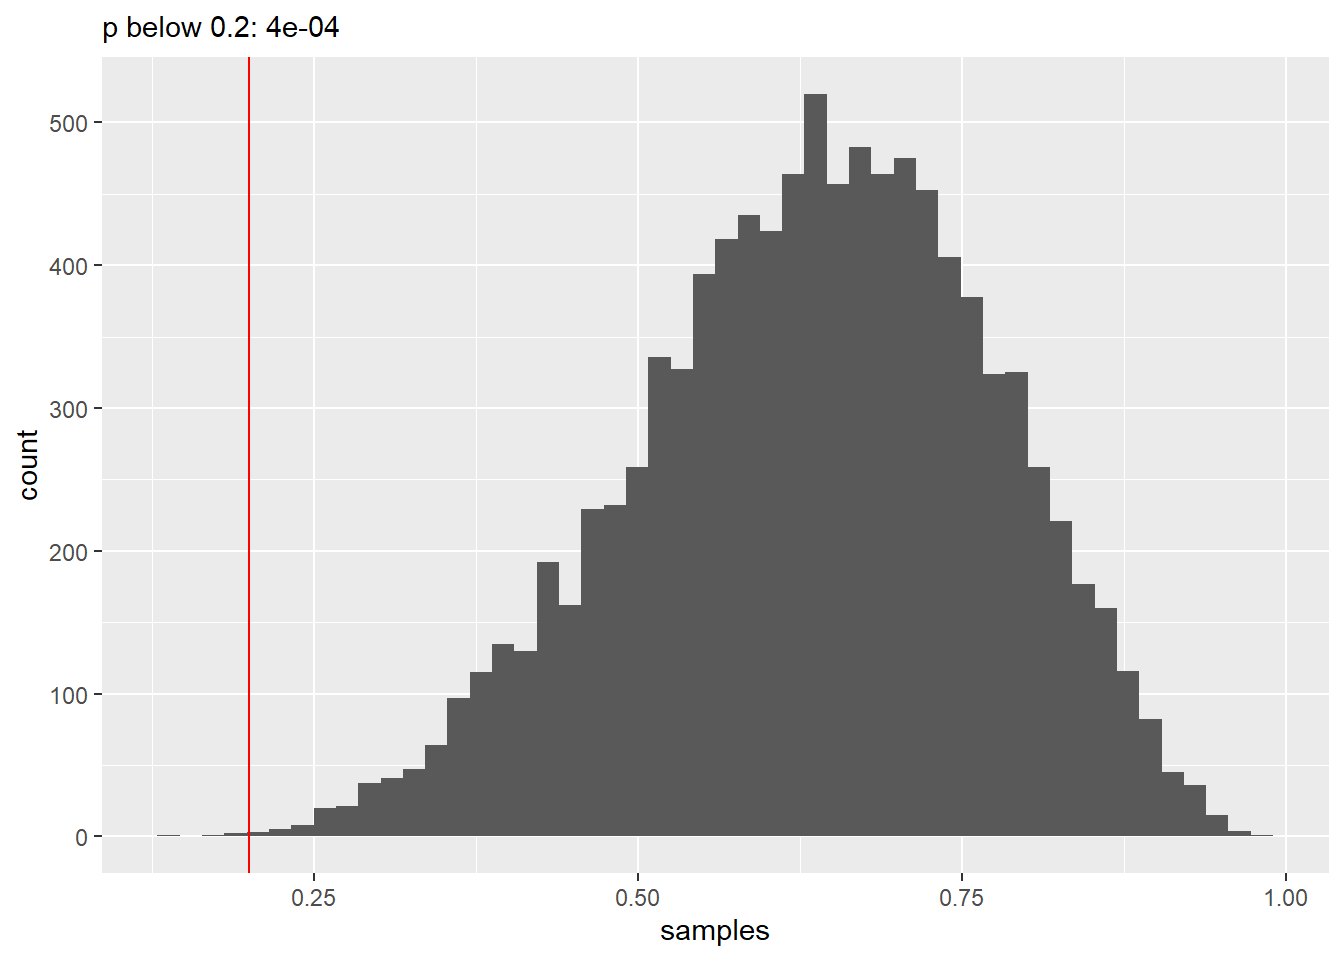
\includegraphics{notes-on-statistical-rethinking_files/figure-latex/3E1-1.pdf}

\hypertarget{e2-1}{%
\subsubsection*{3E2}\label{e2-1}}
\addcontentsline{toc}{subsubsection}{3E2}

How much posterior probability lies below p = 0.8?

\begin{Shaded}
\begin{Highlighting}[]
\KeywordTok{ggplot}\NormalTok{(}\DataTypeTok{data=}\OtherTok{NULL}\NormalTok{, }\KeywordTok{aes}\NormalTok{(}\DataTypeTok{x=}\NormalTok{samples)) }\OperatorTok{+}\StringTok{ }
\StringTok{  }\KeywordTok{geom\_histogram}\NormalTok{(}\DataTypeTok{bins=}\DecValTok{50}\NormalTok{) }\OperatorTok{+}\StringTok{ }
\StringTok{  }\KeywordTok{geom\_vline}\NormalTok{(}\DataTypeTok{xintercept =} \FloatTok{0.8}\NormalTok{, }\DataTypeTok{color=}\StringTok{"red"}\NormalTok{) }\OperatorTok{+}\StringTok{ }
\StringTok{  }\KeywordTok{labs}\NormalTok{(}\DataTypeTok{subtitle =}\NormalTok{ glue}\OperatorTok{::}\KeywordTok{glue}\NormalTok{(}\StringTok{"p below 0.8: \{mean(samples \textless{} 0.8)\}"}\NormalTok{))}
\end{Highlighting}
\end{Shaded}

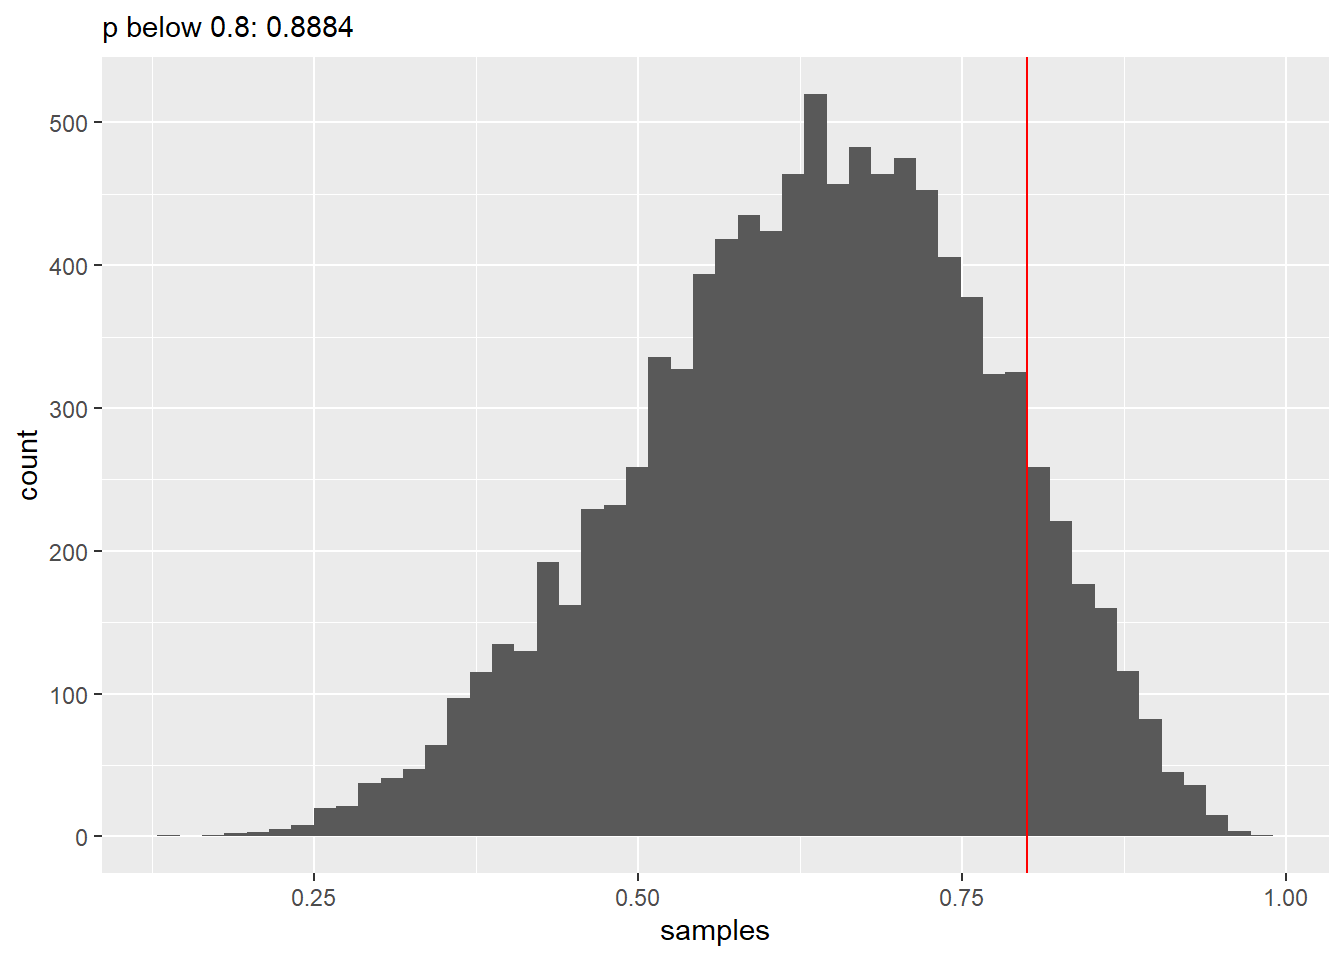
\includegraphics{notes-on-statistical-rethinking_files/figure-latex/3E2-1.pdf}

\hypertarget{e3-1}{%
\subsubsection*{3E3}\label{e3-1}}
\addcontentsline{toc}{subsubsection}{3E3}

How much posterior probability lies between p = 0.2 and p = 0.8?

\begin{Shaded}
\begin{Highlighting}[]
\KeywordTok{ggplot}\NormalTok{(}\DataTypeTok{data=}\OtherTok{NULL}\NormalTok{, }\KeywordTok{aes}\NormalTok{(}\DataTypeTok{x=}\NormalTok{samples)) }\OperatorTok{+}\StringTok{ }
\StringTok{  }\KeywordTok{geom\_histogram}\NormalTok{(}\DataTypeTok{bins=}\DecValTok{50}\NormalTok{) }\OperatorTok{+}\StringTok{ }
\StringTok{  }\KeywordTok{geom\_vline}\NormalTok{(}\DataTypeTok{xintercept =} \KeywordTok{c}\NormalTok{(}\FloatTok{0.2}\NormalTok{, }\FloatTok{0.8}\NormalTok{), }\DataTypeTok{color=}\StringTok{"red"}\NormalTok{) }\OperatorTok{+}\StringTok{ }
\StringTok{  }\KeywordTok{labs}\NormalTok{(}\DataTypeTok{subtitle =}\NormalTok{ glue}\OperatorTok{::}\KeywordTok{glue}\NormalTok{(}\StringTok{"p between 0.2 and 0.8: \{mean(samples \textless{} 0.8 \& samples \textgreater{} 0.2)\}"}\NormalTok{))}
\end{Highlighting}
\end{Shaded}

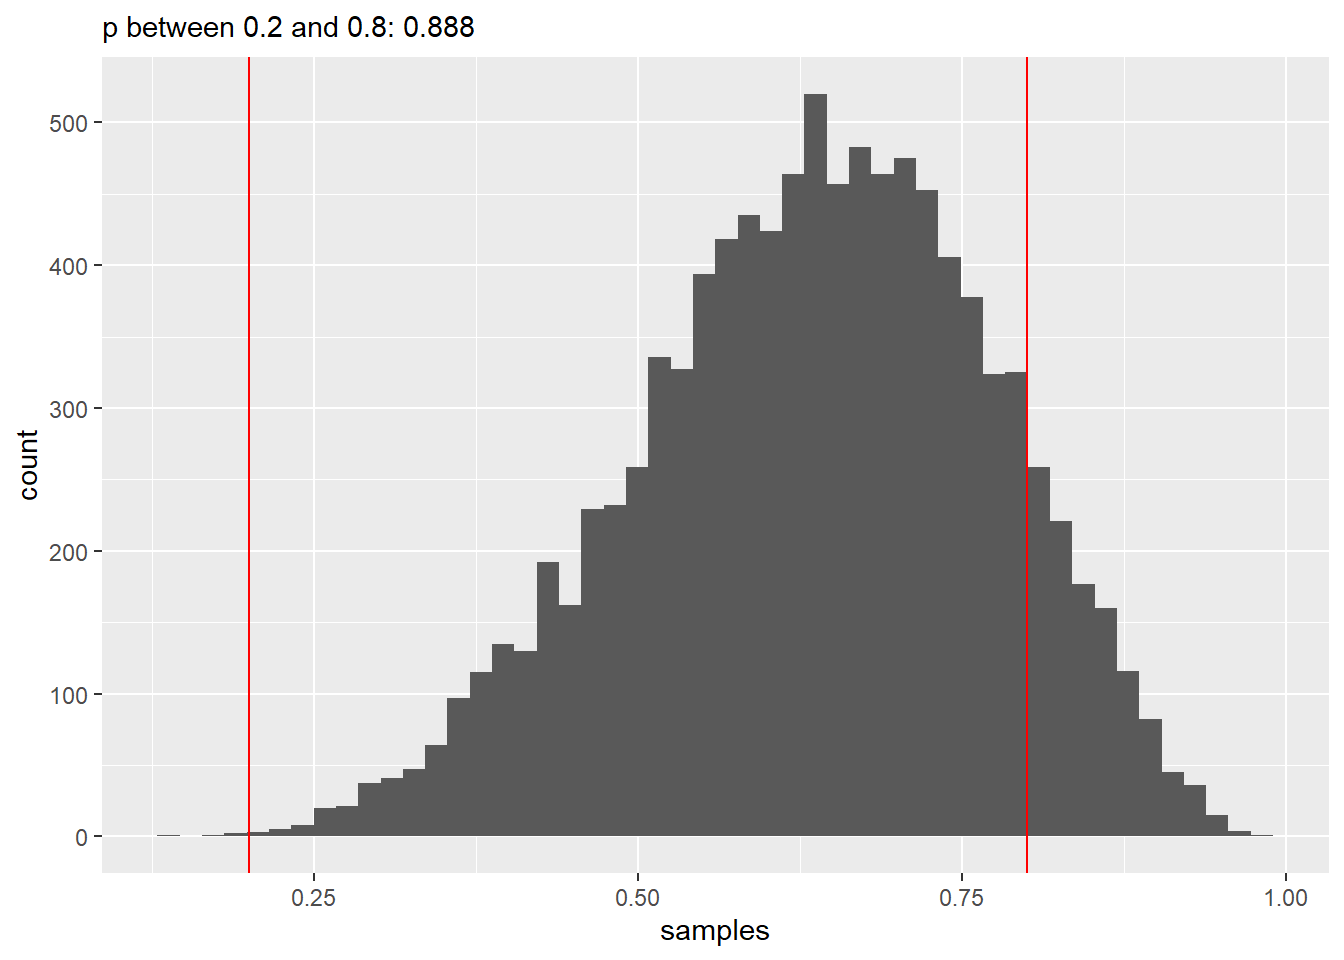
\includegraphics{notes-on-statistical-rethinking_files/figure-latex/3E3-1.pdf}

\hypertarget{e4-1}{%
\subsubsection*{3E4}\label{e4-1}}
\addcontentsline{toc}{subsubsection}{3E4}

20\% of the posterior probability lies below which value of p?

\begin{Shaded}
\begin{Highlighting}[]
\NormalTok{q20 \textless{}{-}}\StringTok{ }\KeywordTok{quantile}\NormalTok{(samples, }\FloatTok{0.2}\NormalTok{)}
\KeywordTok{ggplot}\NormalTok{(}\DataTypeTok{data=}\OtherTok{NULL}\NormalTok{, }\KeywordTok{aes}\NormalTok{(}\DataTypeTok{x=}\NormalTok{samples)) }\OperatorTok{+}\StringTok{ }
\StringTok{  }\KeywordTok{geom\_histogram}\NormalTok{(}\DataTypeTok{bins=}\DecValTok{50}\NormalTok{) }\OperatorTok{+}\StringTok{ }
\StringTok{  }\KeywordTok{geom\_vline}\NormalTok{(}\DataTypeTok{xintercept =}\NormalTok{ q20, }\DataTypeTok{color=}\StringTok{"red"}\NormalTok{) }\OperatorTok{+}\StringTok{ }
\StringTok{  }\KeywordTok{labs}\NormalTok{(}\DataTypeTok{subtitle =}\NormalTok{ glue}\OperatorTok{::}\KeywordTok{glue}\NormalTok{(}\StringTok{"20\% of the posterior probability lies below \{round(q20, 2)\}"}\NormalTok{))}
\end{Highlighting}
\end{Shaded}

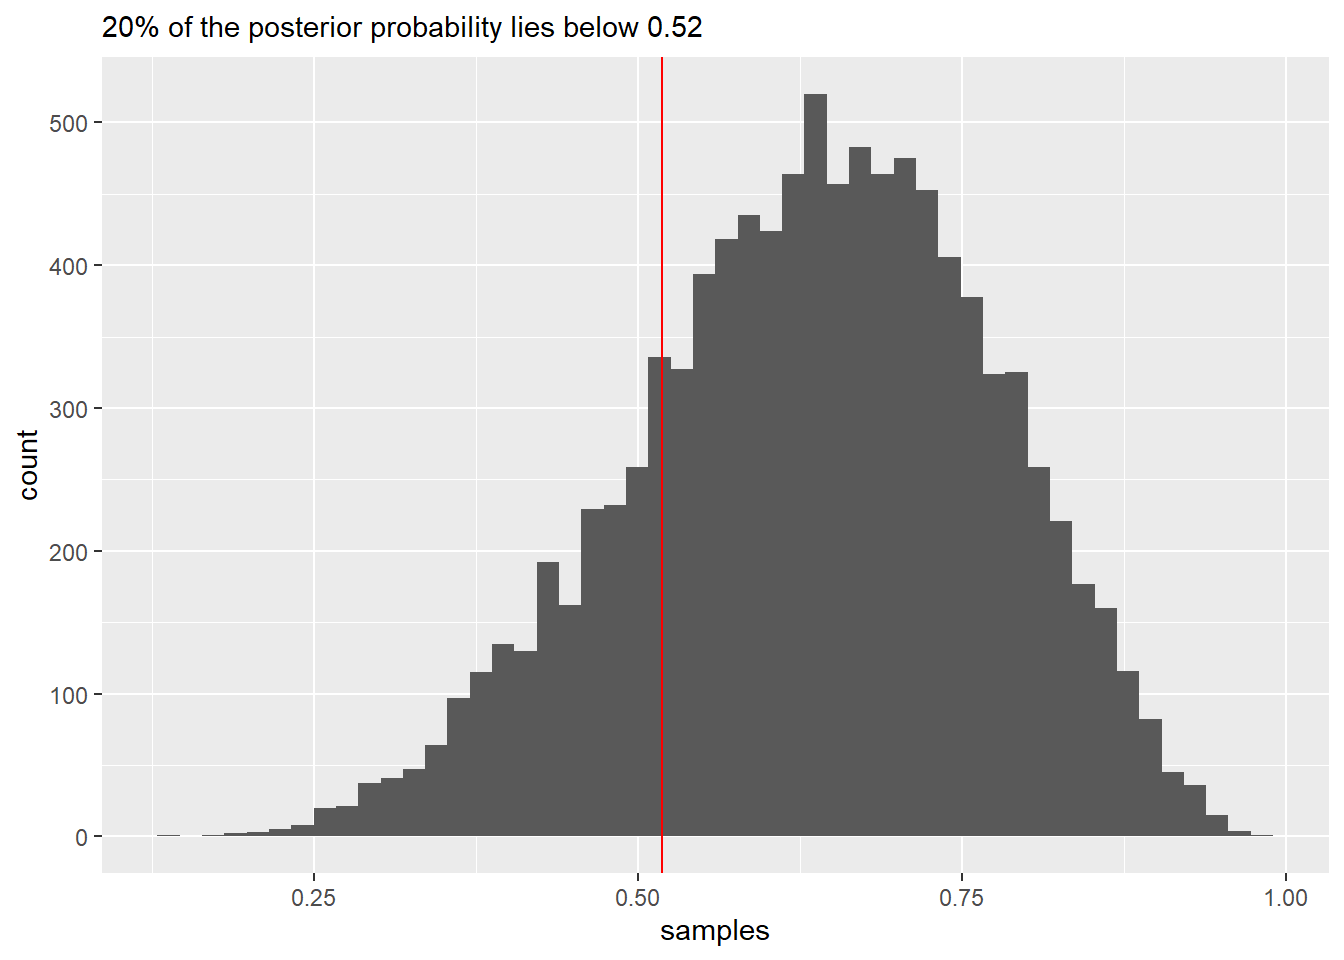
\includegraphics{notes-on-statistical-rethinking_files/figure-latex/3E4-1.pdf}

\hypertarget{e5}{%
\subsubsection*{3E5}\label{e5}}
\addcontentsline{toc}{subsubsection}{3E5}

20\% of the posterior probability lies above which value of p?

\begin{Shaded}
\begin{Highlighting}[]
\NormalTok{q80 \textless{}{-}}\StringTok{ }\KeywordTok{quantile}\NormalTok{(samples, }\FloatTok{0.8}\NormalTok{)}
\KeywordTok{ggplot}\NormalTok{(}\DataTypeTok{data=}\OtherTok{NULL}\NormalTok{, }\KeywordTok{aes}\NormalTok{(}\DataTypeTok{x=}\NormalTok{samples)) }\OperatorTok{+}\StringTok{ }
\StringTok{  }\KeywordTok{geom\_histogram}\NormalTok{(}\DataTypeTok{bins=}\DecValTok{50}\NormalTok{) }\OperatorTok{+}\StringTok{ }
\StringTok{  }\KeywordTok{geom\_vline}\NormalTok{(}\DataTypeTok{xintercept =}\NormalTok{ q80, }\DataTypeTok{color=}\StringTok{"red"}\NormalTok{) }\OperatorTok{+}\StringTok{ }
\StringTok{  }\KeywordTok{labs}\NormalTok{(}\DataTypeTok{subtitle =}\NormalTok{ glue}\OperatorTok{::}\KeywordTok{glue}\NormalTok{(}\StringTok{"20\% of the posterior probability lies above \{round(q80, 2)\}"}\NormalTok{))}
\end{Highlighting}
\end{Shaded}

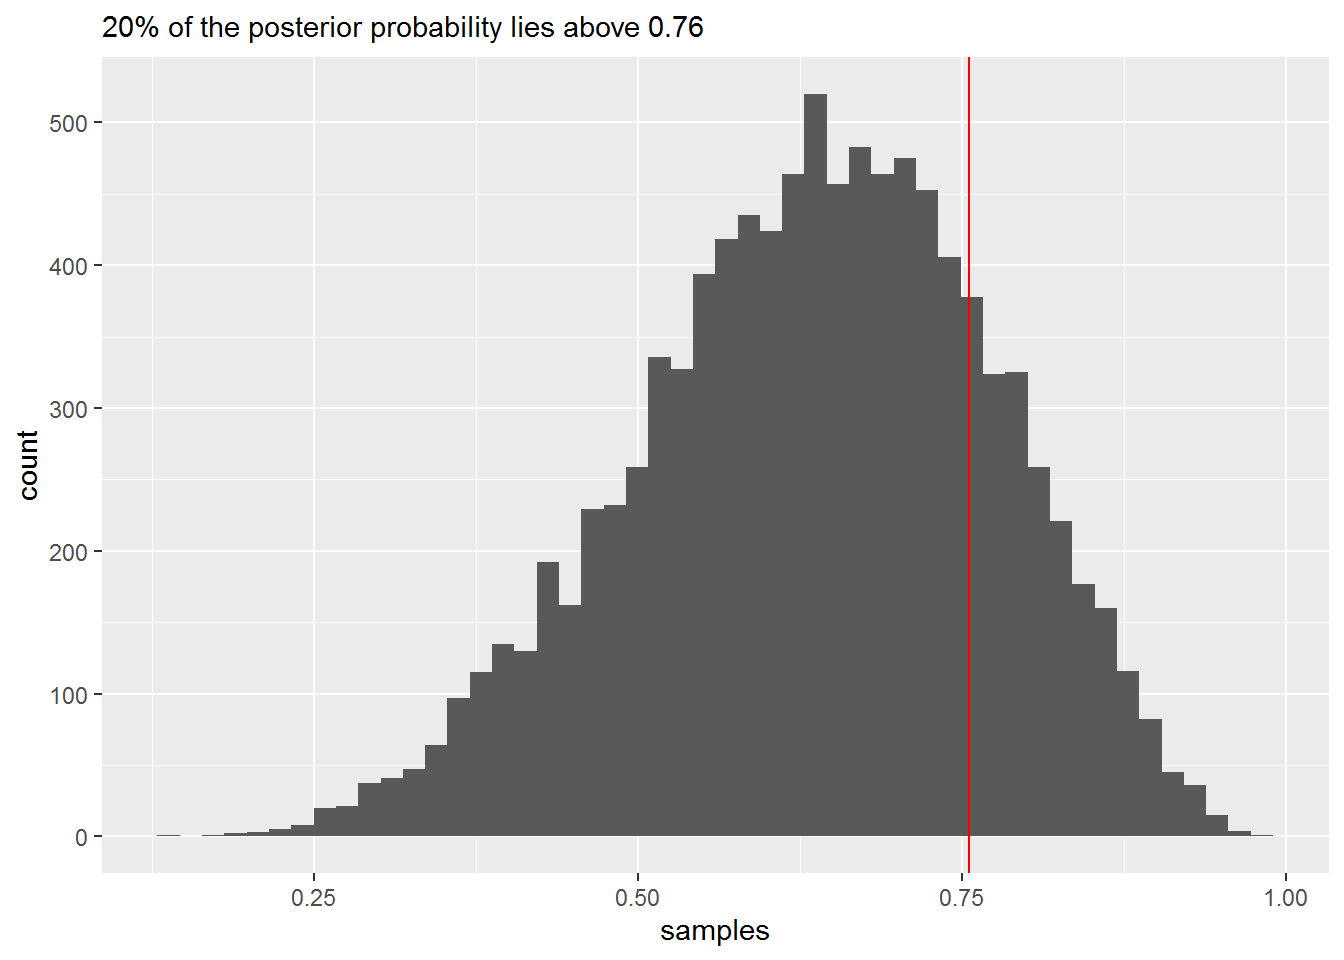
\includegraphics{notes-on-statistical-rethinking_files/figure-latex/3E5-1.pdf}

\hypertarget{e6}{%
\subsubsection*{3E6}\label{e6}}
\addcontentsline{toc}{subsubsection}{3E6}

Which values of p contain the narrowest interval equal to 66\% of the posterior probability?

\begin{Shaded}
\begin{Highlighting}[]
\NormalTok{hpdi66 \textless{}{-}}\StringTok{ }\KeywordTok{HPDI}\NormalTok{(samples, }\FloatTok{0.66}\NormalTok{)}
\KeywordTok{ggplot}\NormalTok{(}\DataTypeTok{data=}\OtherTok{NULL}\NormalTok{, }\KeywordTok{aes}\NormalTok{(}\DataTypeTok{x=}\NormalTok{samples)) }\OperatorTok{+}\StringTok{ }
\StringTok{  }\KeywordTok{geom\_histogram}\NormalTok{(}\DataTypeTok{bins=}\DecValTok{50}\NormalTok{) }\OperatorTok{+}\StringTok{ }
\StringTok{  }\KeywordTok{geom\_vline}\NormalTok{(}\DataTypeTok{xintercept =}\NormalTok{ hpdi66, }\DataTypeTok{color=}\StringTok{"red"}\NormalTok{) }\OperatorTok{+}\StringTok{ }
\StringTok{  }\KeywordTok{labs}\NormalTok{(}\DataTypeTok{subtitle =}\NormalTok{ glue}\OperatorTok{::}\KeywordTok{glue}\NormalTok{(}\StringTok{"Narrowest interval equal to 66\% of the posterior probability is \{round(hpdi66[1], 3)\}..\{round(hpdi66[2], 3)\}"}\NormalTok{))}
\end{Highlighting}
\end{Shaded}

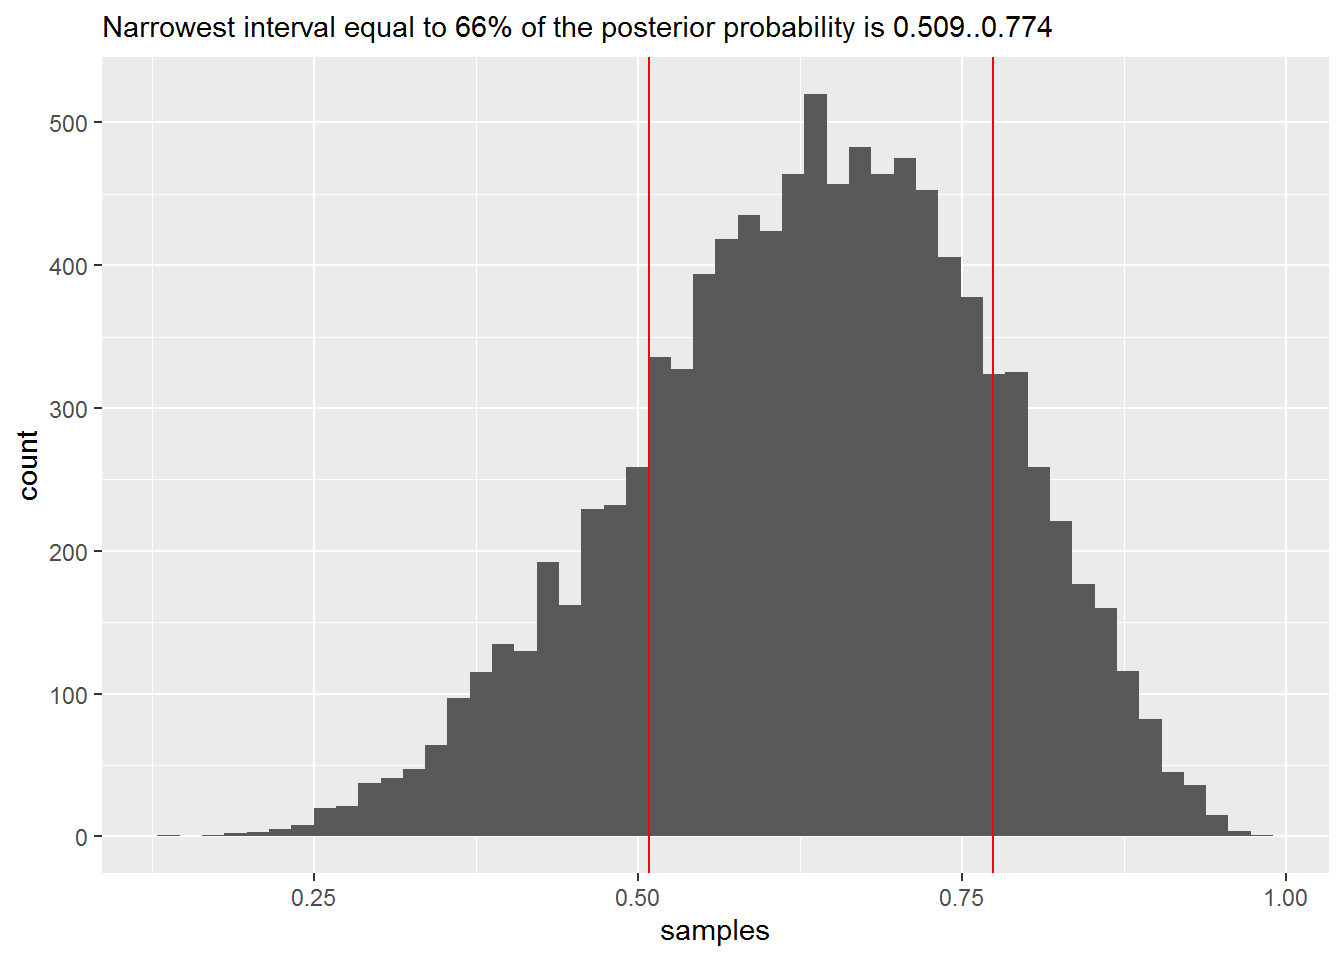
\includegraphics{notes-on-statistical-rethinking_files/figure-latex/3E6-1.pdf}

\hypertarget{e7}{%
\subsubsection*{3E7}\label{e7}}
\addcontentsline{toc}{subsubsection}{3E7}

Which values of p contain 66\% of the posterior probability, assuming equal posterior probability both below and above the interval?

\begin{Shaded}
\begin{Highlighting}[]
\NormalTok{pi66 \textless{}{-}}\StringTok{ }\KeywordTok{PI}\NormalTok{(samples, }\FloatTok{0.66}\NormalTok{)}
\KeywordTok{ggplot}\NormalTok{(}\DataTypeTok{data=}\OtherTok{NULL}\NormalTok{, }\KeywordTok{aes}\NormalTok{(}\DataTypeTok{x=}\NormalTok{samples)) }\OperatorTok{+}\StringTok{ }
\StringTok{  }\KeywordTok{geom\_histogram}\NormalTok{(}\DataTypeTok{bins=}\DecValTok{50}\NormalTok{) }\OperatorTok{+}\StringTok{ }
\StringTok{  }\KeywordTok{geom\_vline}\NormalTok{(}\DataTypeTok{xintercept =}\NormalTok{ pi66, }\DataTypeTok{color=}\StringTok{"red"}\NormalTok{) }\OperatorTok{+}\StringTok{ }
\StringTok{  }\KeywordTok{labs}\NormalTok{(}\DataTypeTok{subtitle =}\NormalTok{ glue}\OperatorTok{::}\KeywordTok{glue}\NormalTok{(}\StringTok{"66\% of the posterior probability, assuming equal posterior probability are between \{round(pi66[1], 3)\}..\{round(pi66[2], 3)\}"}\NormalTok{))}
\end{Highlighting}
\end{Shaded}

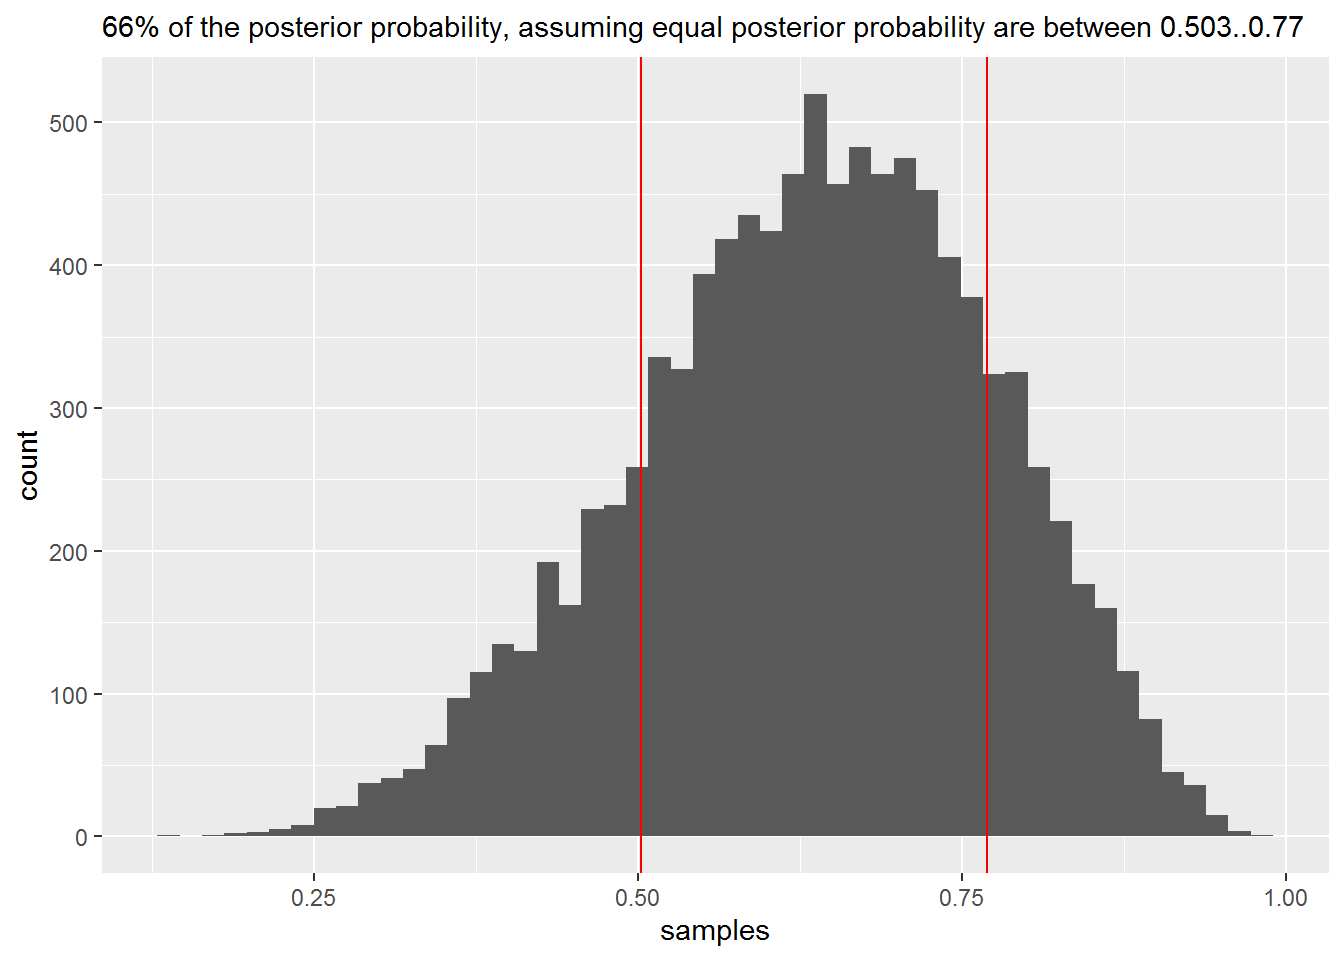
\includegraphics{notes-on-statistical-rethinking_files/figure-latex/3E7-1.pdf}

\hypertarget{m1-1}{%
\subsubsection*{3M1}\label{m1-1}}
\addcontentsline{toc}{subsubsection}{3M1}

Suppose the globe tossing data had turned out to be 8 water in 15 tosses. Construct the posterior distribution, using grid approximation. Use the same flat prior as before.

\begin{Shaded}
\begin{Highlighting}[]
\NormalTok{p\_grid \textless{}{-}}\StringTok{ }\KeywordTok{seq}\NormalTok{(}\DataTypeTok{from=}\DecValTok{0}\NormalTok{, }\DataTypeTok{to=}\DecValTok{1}\NormalTok{, }\DataTypeTok{length.out=}\DecValTok{1000}\NormalTok{)}
\NormalTok{prior \textless{}{-}}\StringTok{ }\KeywordTok{rep}\NormalTok{(}\DecValTok{1}\NormalTok{,}\DecValTok{1000}\NormalTok{)}
\NormalTok{likelihood \textless{}{-}}\StringTok{ }\KeywordTok{dbinom}\NormalTok{(}\DecValTok{8}\NormalTok{, }\DataTypeTok{size=}\DecValTok{15}\NormalTok{, }\DataTypeTok{prob=}\NormalTok{p\_grid)}
\NormalTok{posterior \textless{}{-}}\StringTok{ }\NormalTok{likelihood }\OperatorTok{*}\StringTok{ }\NormalTok{prior}
\NormalTok{posterior \textless{}{-}}\StringTok{ }\NormalTok{posterior }\OperatorTok{/}\StringTok{ }\KeywordTok{sum}\NormalTok{(posterior)}

\KeywordTok{ggplot}\NormalTok{(}\DataTypeTok{data=}\OtherTok{NULL}\NormalTok{, }\KeywordTok{aes}\NormalTok{(}\DataTypeTok{x=}\NormalTok{p\_grid, }\DataTypeTok{y=}\NormalTok{posterior)) }\OperatorTok{+}\StringTok{ }
\StringTok{  }\KeywordTok{geom\_line}\NormalTok{() }\OperatorTok{+}
\StringTok{  }\KeywordTok{labs}\NormalTok{(}\DataTypeTok{subtitle=}\StringTok{"8 water in 15 tosses"}\NormalTok{)}
\end{Highlighting}
\end{Shaded}

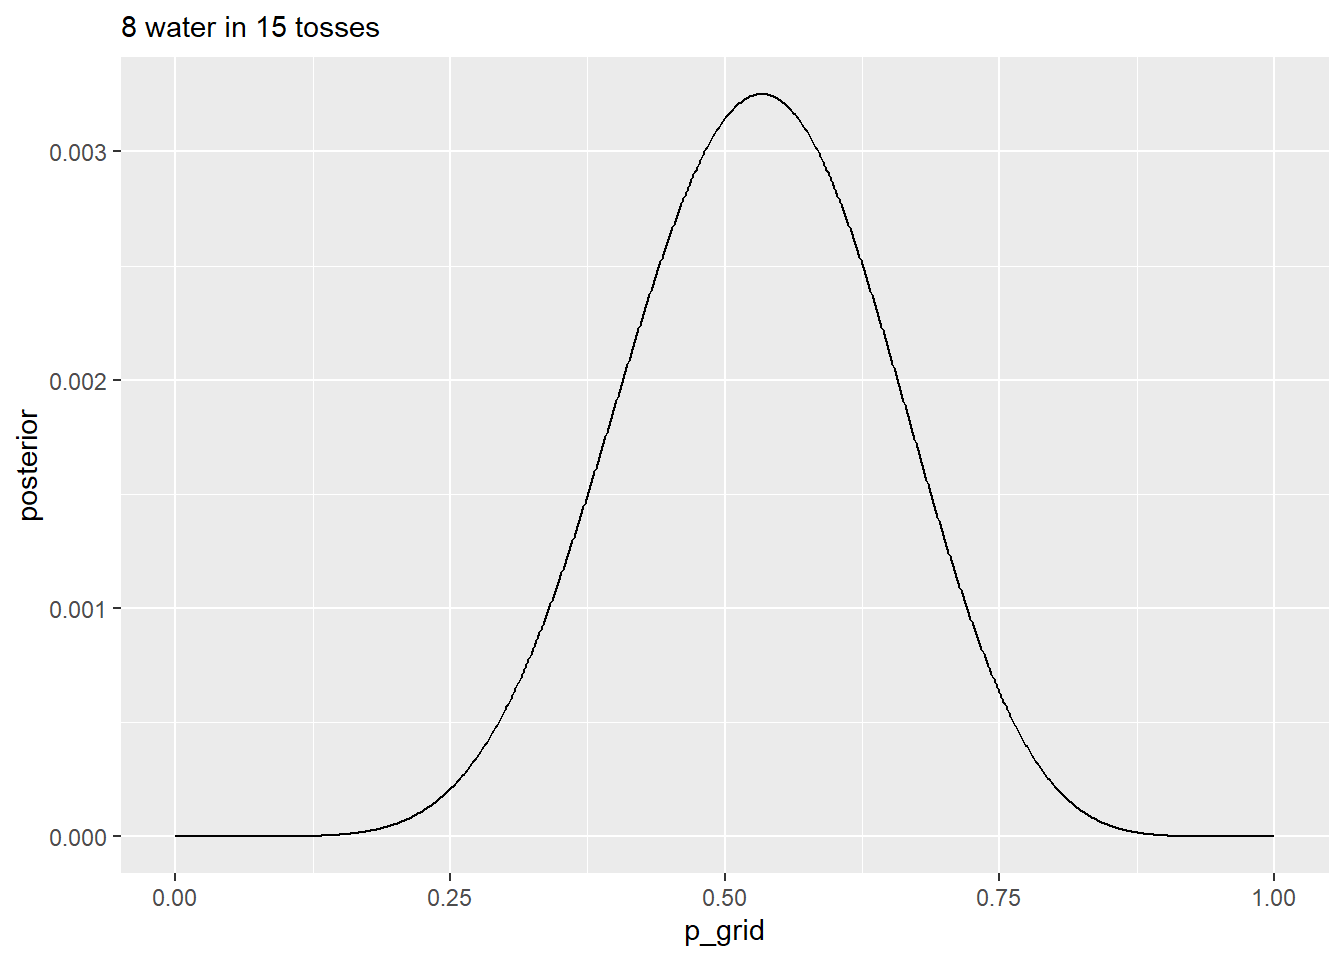
\includegraphics{notes-on-statistical-rethinking_files/figure-latex/3M1-1.pdf}

\hypertarget{m2-1}{%
\subsubsection*{3M2}\label{m2-1}}
\addcontentsline{toc}{subsubsection}{3M2}

Draw 10,000 samples from the grid approximation from above. Then use the samples to calculate the 90\% HPDI for p.

\begin{Shaded}
\begin{Highlighting}[]
\KeywordTok{set.seed}\NormalTok{(}\DecValTok{100}\NormalTok{)}
\NormalTok{samples \textless{}{-}}\StringTok{ }\KeywordTok{sample}\NormalTok{(p\_grid, }\DataTypeTok{prob=}\NormalTok{posterior, }\DataTypeTok{size=}\FloatTok{1e4}\NormalTok{, }\DataTypeTok{replace=}\OtherTok{TRUE}\NormalTok{)}

\NormalTok{hpdi90 \textless{}{-}}\StringTok{ }\KeywordTok{HPDI}\NormalTok{(samples, }\FloatTok{0.9}\NormalTok{)}
\KeywordTok{ggplot}\NormalTok{(}\DataTypeTok{data=}\OtherTok{NULL}\NormalTok{, }\KeywordTok{aes}\NormalTok{(}\DataTypeTok{x=}\NormalTok{samples)) }\OperatorTok{+}\StringTok{ }
\StringTok{  }\KeywordTok{geom\_histogram}\NormalTok{(}\DataTypeTok{bins=}\DecValTok{50}\NormalTok{) }\OperatorTok{+}\StringTok{ }
\StringTok{  }\KeywordTok{geom\_vline}\NormalTok{(}\DataTypeTok{xintercept =}\NormalTok{ hpdi90, }\DataTypeTok{color=}\StringTok{"red"}\NormalTok{) }\OperatorTok{+}\StringTok{ }
\StringTok{  }\KeywordTok{labs}\NormalTok{(}\DataTypeTok{subtitle =}\NormalTok{ glue}\OperatorTok{::}\KeywordTok{glue}\NormalTok{(}\StringTok{"HPDI 90\% is \{round(hpdi66[1], 3)\}..\{round(hpdi66[2], 3)\}"}\NormalTok{))}
\end{Highlighting}
\end{Shaded}

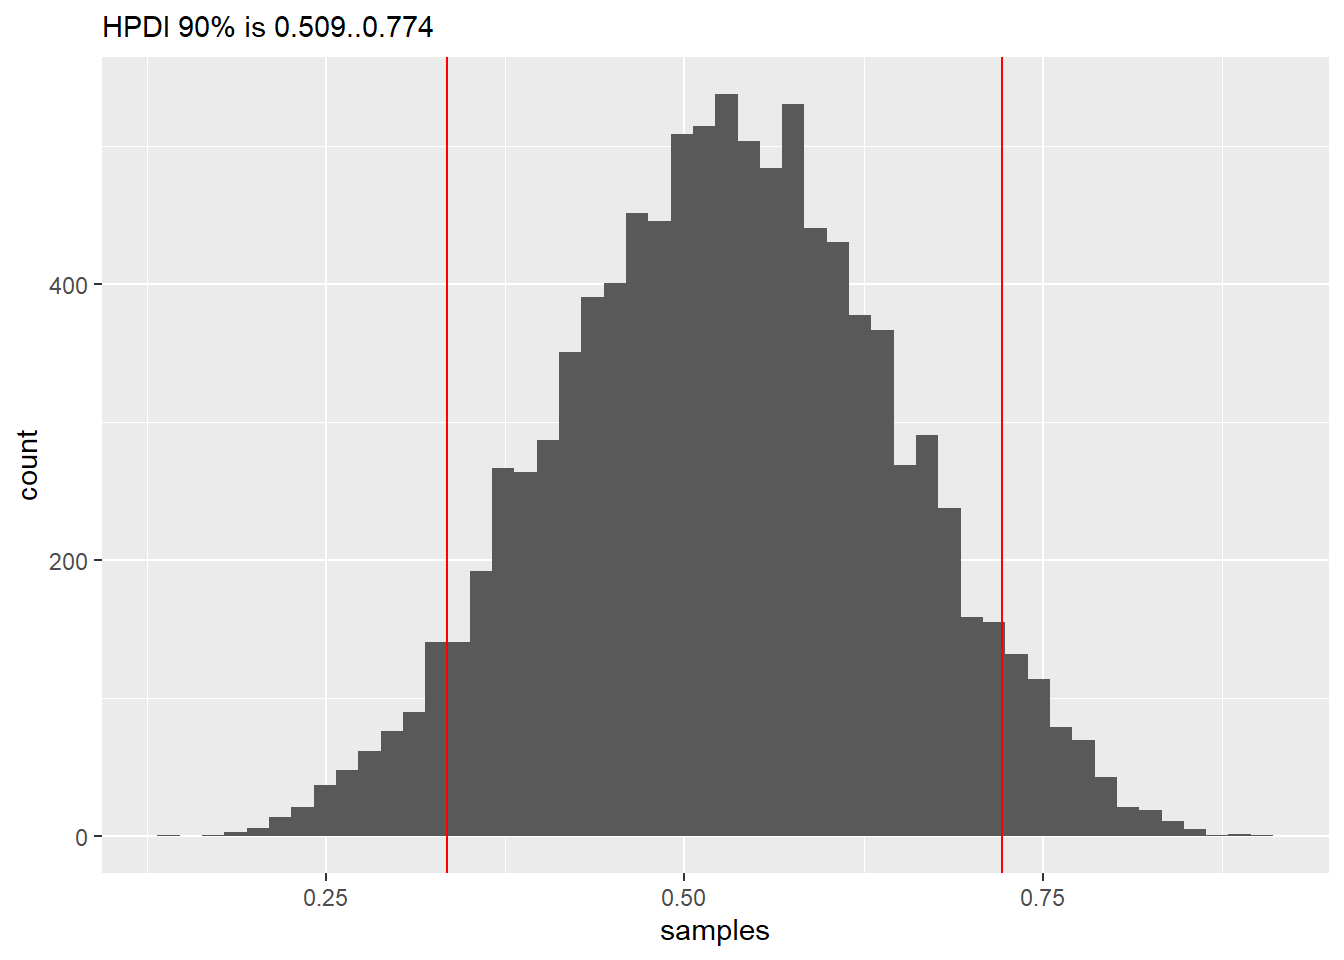
\includegraphics{notes-on-statistical-rethinking_files/figure-latex/3M2-1.pdf}

\hypertarget{m3-1}{%
\subsubsection*{3M3}\label{m3-1}}
\addcontentsline{toc}{subsubsection}{3M3}

Construct a posterior predictive check for this model and data. This means simulate the distribution of samples, averaging over the posterior uncertainty in p . What is the probability of observing 8 water in 15 tosses?

\begin{Shaded}
\begin{Highlighting}[]
\NormalTok{predicted\_water8\_}\DecValTok{15}\NormalTok{ \textless{}{-}}\StringTok{ }
\StringTok{  }\KeywordTok{tibble}\NormalTok{(}\DataTypeTok{N =} \KeywordTok{rbinom}\NormalTok{(}\KeywordTok{length}\NormalTok{(samples), }\DataTypeTok{size=}\DecValTok{15}\NormalTok{, }\DataTypeTok{prob=}\NormalTok{samples)) }\OperatorTok{\%\textgreater{}\%}
\StringTok{  }\KeywordTok{group\_by}\NormalTok{(N) }\OperatorTok{\%\textgreater{}\%}
\StringTok{  }\KeywordTok{summarize}\NormalTok{(}\DataTypeTok{count =} \KeywordTok{n}\NormalTok{(), }\DataTypeTok{.groups =} \StringTok{\textquotesingle{}drop\textquotesingle{}}\NormalTok{)  }\OperatorTok{\%\textgreater{}\%}
\StringTok{  }\KeywordTok{ungroup}\NormalTok{() }\OperatorTok{\%\textgreater{}\%}
\StringTok{  }\KeywordTok{mutate}\NormalTok{(}\DataTypeTok{p =}\NormalTok{ count }\OperatorTok{/}\StringTok{ }\KeywordTok{sum}\NormalTok{(count))}
  
\NormalTok{p8 \textless{}{-}}\StringTok{ }
\StringTok{  }\NormalTok{predicted\_water8\_}\DecValTok{15} \OperatorTok{\%\textgreater{}\%}
\StringTok{  }\KeywordTok{filter}\NormalTok{(N }\OperatorTok{==}\StringTok{ }\DecValTok{8}\NormalTok{) }\OperatorTok{\%\textgreater{}\%}
\StringTok{  }\KeywordTok{pull}\NormalTok{(p)}

\KeywordTok{ggplot}\NormalTok{(predicted\_water8\_}\DecValTok{15}\NormalTok{, }\KeywordTok{aes}\NormalTok{(}\DataTypeTok{x=}\NormalTok{N, }\DataTypeTok{y=}\NormalTok{ p)) }\OperatorTok{+}\StringTok{ }
\StringTok{    }\KeywordTok{geom\_point}\NormalTok{() }\OperatorTok{+}\StringTok{ }
\StringTok{  }\KeywordTok{labs}\NormalTok{(}\DataTypeTok{subtitle =}\NormalTok{ glue}\OperatorTok{::}\KeywordTok{glue}\NormalTok{(}\StringTok{"The probability of observing 8 water in 15 tosses is \{p8\}"}\NormalTok{))}
\end{Highlighting}
\end{Shaded}

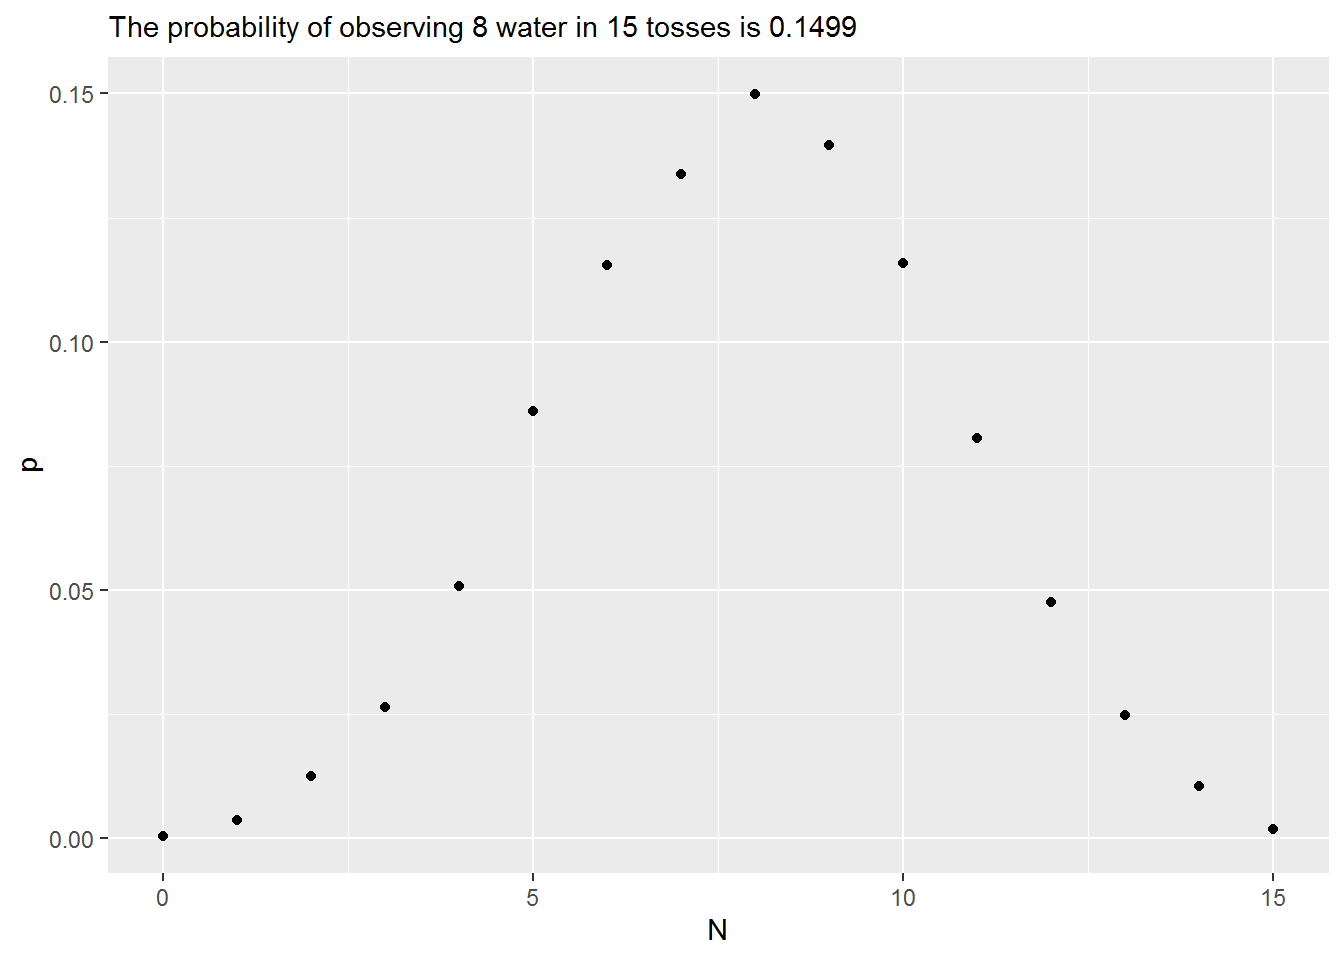
\includegraphics{notes-on-statistical-rethinking_files/figure-latex/3M3-1.pdf}

\hypertarget{m4-1}{%
\subsubsection*{3M4}\label{m4-1}}
\addcontentsline{toc}{subsubsection}{3M4}

Using the posterior distribution constructed from the new (8/15) data, now calculate the probability of observing 6 water in 9 tosses.

\begin{Shaded}
\begin{Highlighting}[]
\NormalTok{predicted\_water6\_}\DecValTok{9}\NormalTok{ \textless{}{-}}\StringTok{ }
\StringTok{  }\KeywordTok{tibble}\NormalTok{(}\DataTypeTok{N =} \KeywordTok{rbinom}\NormalTok{(}\KeywordTok{length}\NormalTok{(samples), }\DataTypeTok{size=}\DecValTok{9}\NormalTok{, }\DataTypeTok{prob=}\NormalTok{samples)) }\OperatorTok{\%\textgreater{}\%}
\StringTok{  }\KeywordTok{group\_by}\NormalTok{(N) }\OperatorTok{\%\textgreater{}\%}
\StringTok{  }\KeywordTok{summarize}\NormalTok{(}\DataTypeTok{count =} \KeywordTok{n}\NormalTok{(), }\DataTypeTok{.groups =} \StringTok{\textquotesingle{}drop\textquotesingle{}}\NormalTok{)  }\OperatorTok{\%\textgreater{}\%}
\StringTok{  }\KeywordTok{ungroup}\NormalTok{() }\OperatorTok{\%\textgreater{}\%}
\StringTok{  }\KeywordTok{mutate}\NormalTok{(}\DataTypeTok{p =}\NormalTok{ count }\OperatorTok{/}\StringTok{ }\KeywordTok{sum}\NormalTok{(count))}
  
\NormalTok{p6 \textless{}{-}}\StringTok{ }
\StringTok{  }\NormalTok{predicted\_water6\_}\DecValTok{9} \OperatorTok{\%\textgreater{}\%}
\StringTok{  }\KeywordTok{filter}\NormalTok{(N }\OperatorTok{==}\StringTok{ }\DecValTok{6}\NormalTok{) }\OperatorTok{\%\textgreater{}\%}
\StringTok{  }\KeywordTok{pull}\NormalTok{(p)}

\KeywordTok{ggplot}\NormalTok{(predicted\_water6\_}\DecValTok{9}\NormalTok{, }\KeywordTok{aes}\NormalTok{(}\DataTypeTok{x=}\NormalTok{N, }\DataTypeTok{y=}\NormalTok{ p)) }\OperatorTok{+}\StringTok{ }
\StringTok{    }\KeywordTok{geom\_point}\NormalTok{() }\OperatorTok{+}\StringTok{ }
\StringTok{  }\KeywordTok{labs}\NormalTok{(}\DataTypeTok{subtitle =}\NormalTok{ glue}\OperatorTok{::}\KeywordTok{glue}\NormalTok{(}\StringTok{"The probability of observing 6 water in 9 tosses is \{p6\}"}\NormalTok{))}
\end{Highlighting}
\end{Shaded}

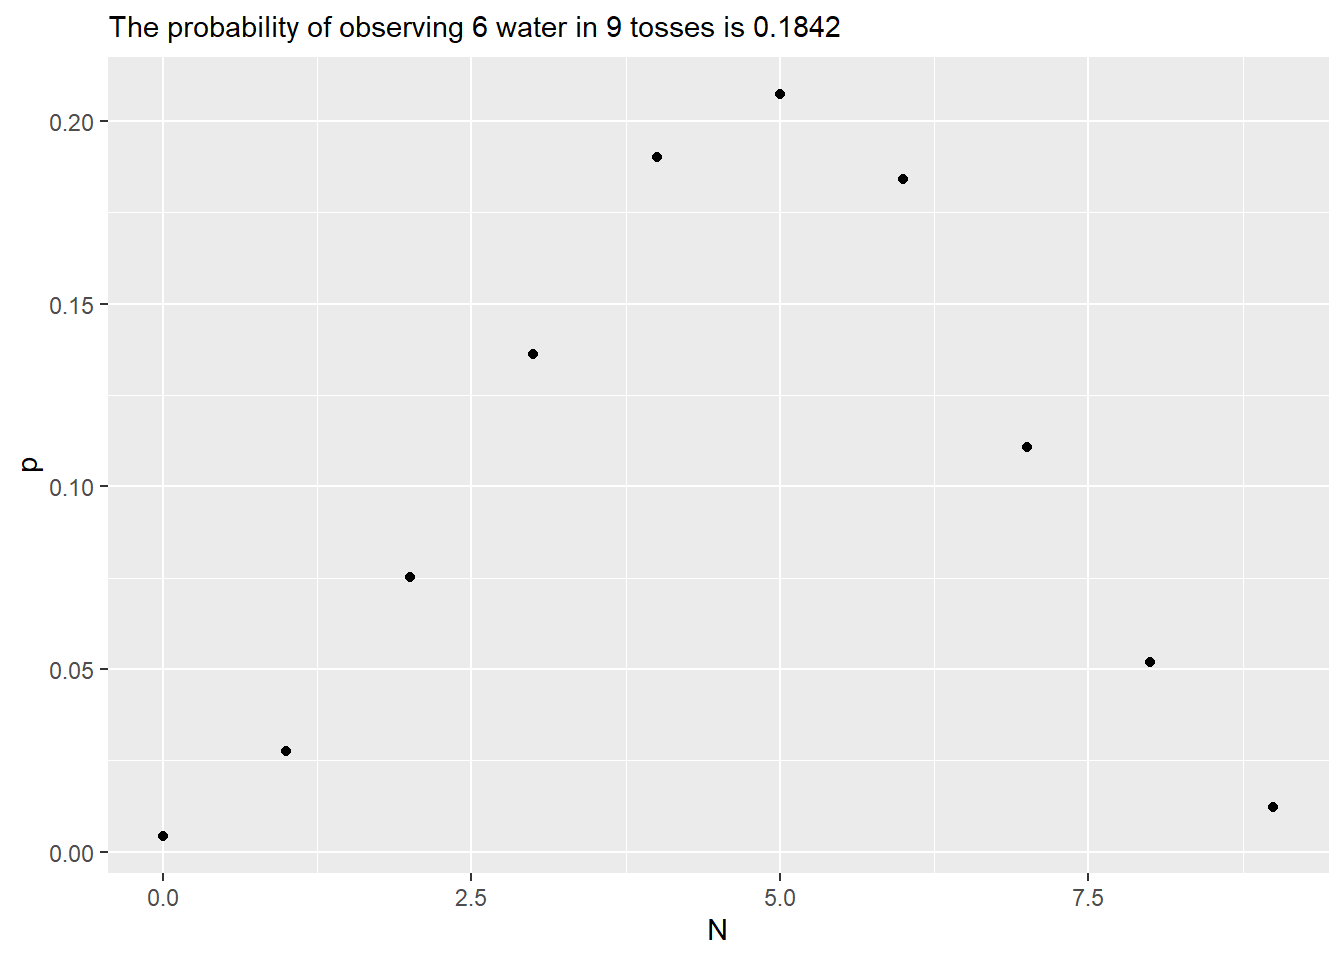
\includegraphics{notes-on-statistical-rethinking_files/figure-latex/3M4-1.pdf}

\hypertarget{m5-1}{%
\subsubsection*{3M5}\label{m5-1}}
\addcontentsline{toc}{subsubsection}{3M5}

Start over at 3M1 , but now use a prior that is zero below p = 0.5 and a constant above p = 0.5. This corresponds to prior information that a majority of the Earth's surface is water. Repeat each problem above and compare the inferences. What difference does the better prior make? If it helps, compare inferences (using both priors) to the true value p = 0.7.

\begin{Shaded}
\begin{Highlighting}[]
\NormalTok{p\_grid \textless{}{-}}\StringTok{ }\KeywordTok{seq}\NormalTok{(}\DataTypeTok{from=}\DecValTok{0}\NormalTok{, }\DataTypeTok{to=}\DecValTok{1}\NormalTok{, }\DataTypeTok{length.out=}\DecValTok{1000}\NormalTok{)}
\NormalTok{prior \textless{}{-}}\StringTok{ }\KeywordTok{as.numeric}\NormalTok{(p\_grid }\OperatorTok{\textgreater{}=}\StringTok{ }\FloatTok{0.5}\NormalTok{)}
\NormalTok{likelihood \textless{}{-}}\StringTok{ }\KeywordTok{dbinom}\NormalTok{(}\DecValTok{8}\NormalTok{, }\DataTypeTok{size=}\DecValTok{15}\NormalTok{, }\DataTypeTok{prob=}\NormalTok{p\_grid)}
\NormalTok{posterior \textless{}{-}}\StringTok{ }\NormalTok{likelihood }\OperatorTok{*}\StringTok{ }\NormalTok{prior}
\NormalTok{posterior \textless{}{-}}\StringTok{ }\NormalTok{posterior }\OperatorTok{/}\StringTok{ }\KeywordTok{sum}\NormalTok{(posterior)}

\KeywordTok{ggplot}\NormalTok{(}\DataTypeTok{data=}\OtherTok{NULL}\NormalTok{, }\KeywordTok{aes}\NormalTok{(}\DataTypeTok{x=}\NormalTok{p\_grid, }\DataTypeTok{y=}\NormalTok{posterior)) }\OperatorTok{+}\StringTok{ }
\StringTok{  }\KeywordTok{geom\_line}\NormalTok{() }\OperatorTok{+}
\StringTok{  }\KeywordTok{labs}\NormalTok{(}\DataTypeTok{subtitle=}\StringTok{"8 water in 15 tosses"}\NormalTok{)}
\end{Highlighting}
\end{Shaded}

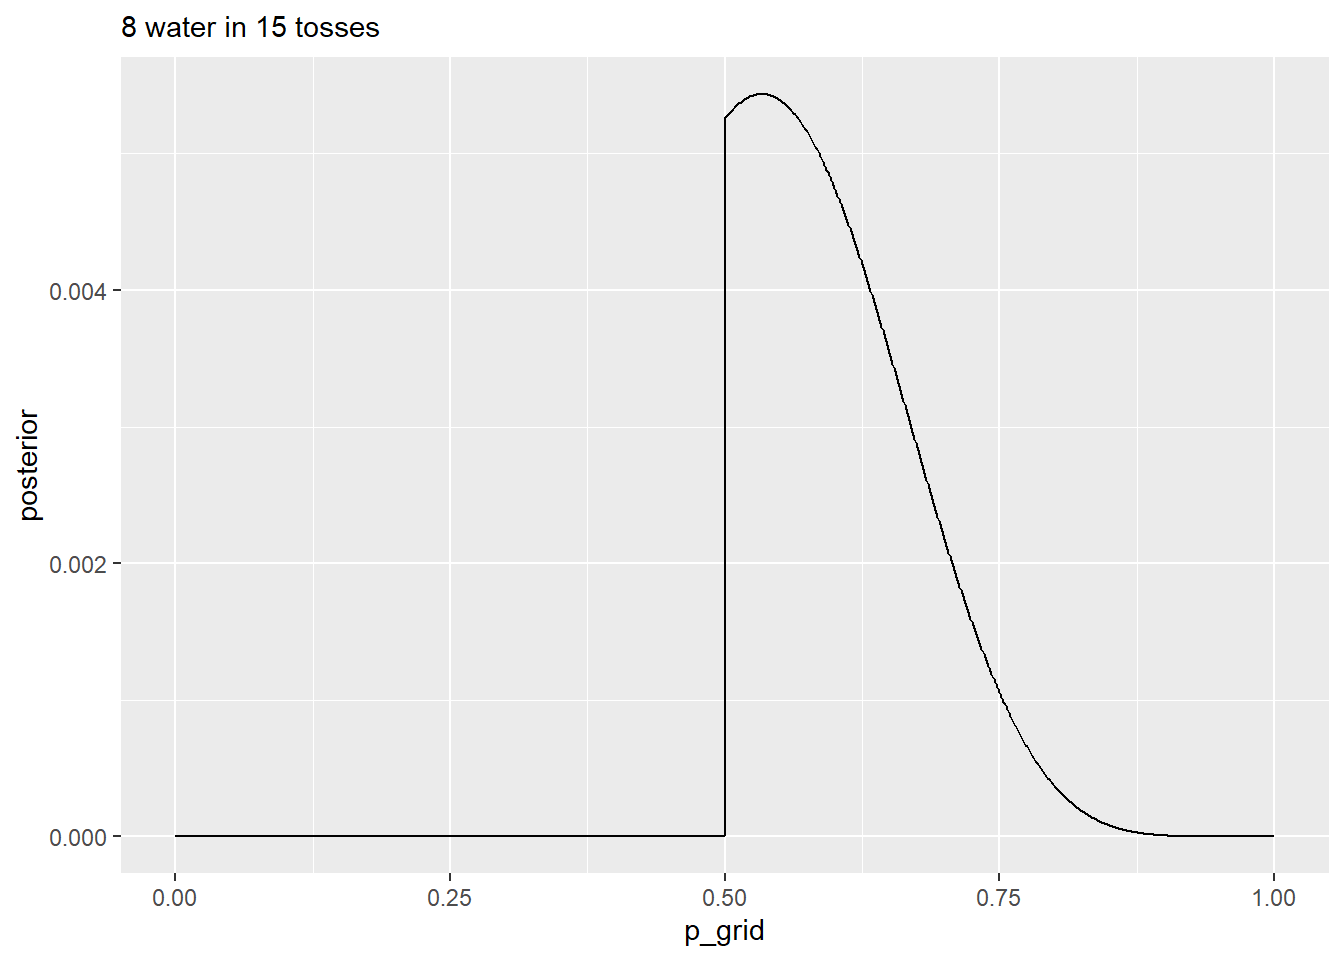
\includegraphics{notes-on-statistical-rethinking_files/figure-latex/3M5-1-1.pdf}

\begin{Shaded}
\begin{Highlighting}[]
\KeywordTok{set.seed}\NormalTok{(}\DecValTok{100}\NormalTok{)}
\NormalTok{samples \textless{}{-}}\StringTok{ }\KeywordTok{sample}\NormalTok{(p\_grid, }\DataTypeTok{prob=}\NormalTok{posterior, }\DataTypeTok{size=}\FloatTok{1e4}\NormalTok{, }\DataTypeTok{replace=}\OtherTok{TRUE}\NormalTok{)}

\NormalTok{hpdi90 \textless{}{-}}\StringTok{ }\KeywordTok{HPDI}\NormalTok{(samples, }\FloatTok{0.9}\NormalTok{)}
\KeywordTok{ggplot}\NormalTok{(}\DataTypeTok{data=}\OtherTok{NULL}\NormalTok{, }\KeywordTok{aes}\NormalTok{(}\DataTypeTok{x=}\NormalTok{samples)) }\OperatorTok{+}\StringTok{ }
\StringTok{  }\KeywordTok{geom\_histogram}\NormalTok{(}\DataTypeTok{bins=}\DecValTok{50}\NormalTok{) }\OperatorTok{+}\StringTok{ }
\StringTok{  }\KeywordTok{geom\_vline}\NormalTok{(}\DataTypeTok{xintercept =}\NormalTok{ hpdi90, }\DataTypeTok{color=}\StringTok{"red"}\NormalTok{) }\OperatorTok{+}\StringTok{ }
\StringTok{  }\KeywordTok{labs}\NormalTok{(}\DataTypeTok{title =} \StringTok{"Remake of 3M2"}\NormalTok{,}
       \DataTypeTok{subtitle =}\NormalTok{ glue}\OperatorTok{::}\KeywordTok{glue}\NormalTok{(}\StringTok{"HPDI 90\% is \{round(hpdi66[1], 3)\}..\{round(hpdi66[2], 3)\}"}\NormalTok{))}
\end{Highlighting}
\end{Shaded}

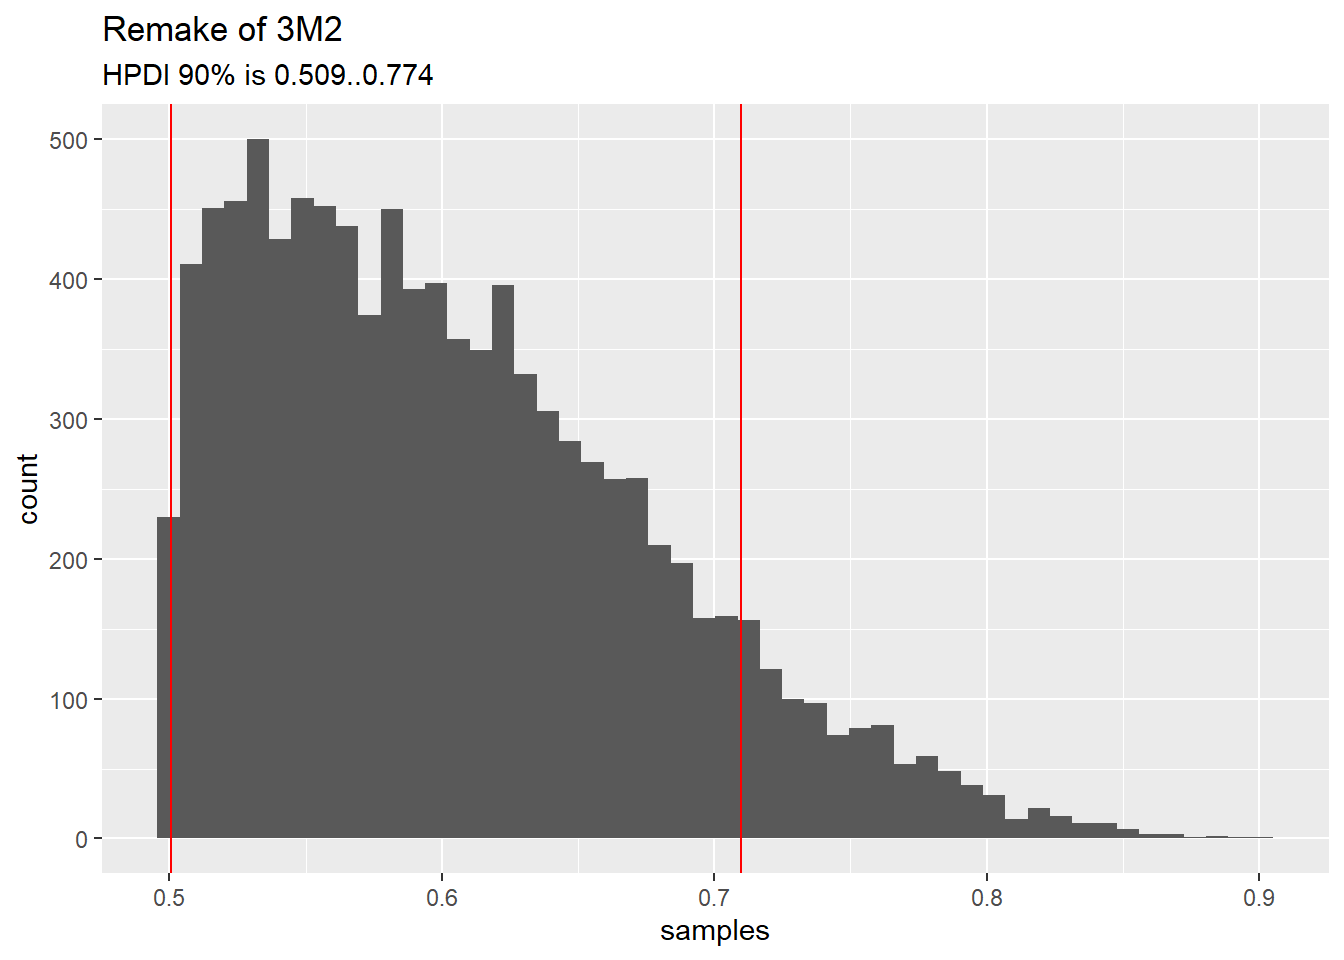
\includegraphics{notes-on-statistical-rethinking_files/figure-latex/3M5-2-1.pdf}

\begin{Shaded}
\begin{Highlighting}[]
\NormalTok{predicted\_water8\_}\DecValTok{15}\NormalTok{\_remake \textless{}{-}}\StringTok{ }
\StringTok{  }\KeywordTok{tibble}\NormalTok{(}\DataTypeTok{N =} \KeywordTok{rbinom}\NormalTok{(}\KeywordTok{length}\NormalTok{(samples), }\DataTypeTok{size=}\DecValTok{15}\NormalTok{, }\DataTypeTok{prob=}\NormalTok{samples)) }\OperatorTok{\%\textgreater{}\%}
\StringTok{  }\KeywordTok{group\_by}\NormalTok{(N) }\OperatorTok{\%\textgreater{}\%}
\StringTok{  }\KeywordTok{summarize}\NormalTok{(}\DataTypeTok{count =} \KeywordTok{n}\NormalTok{(), }\DataTypeTok{.groups =} \StringTok{\textquotesingle{}drop\textquotesingle{}}\NormalTok{)  }\OperatorTok{\%\textgreater{}\%}
\StringTok{  }\KeywordTok{ungroup}\NormalTok{() }\OperatorTok{\%\textgreater{}\%}
\StringTok{  }\KeywordTok{mutate}\NormalTok{(}\DataTypeTok{p =}\NormalTok{ count }\OperatorTok{/}\StringTok{ }\KeywordTok{sum}\NormalTok{(count))}
  
\NormalTok{p8 \textless{}{-}}\StringTok{ }
\StringTok{  }\NormalTok{predicted\_water8\_}\DecValTok{15}\NormalTok{\_remake }\OperatorTok{\%\textgreater{}\%}
\StringTok{  }\KeywordTok{filter}\NormalTok{(N }\OperatorTok{==}\StringTok{ }\DecValTok{8}\NormalTok{) }\OperatorTok{\%\textgreater{}\%}
\StringTok{  }\KeywordTok{pull}\NormalTok{(p)}

\KeywordTok{ggplot}\NormalTok{(predicted\_water8\_}\DecValTok{15}\NormalTok{\_remake, }\KeywordTok{aes}\NormalTok{(}\DataTypeTok{x=}\NormalTok{N, }\DataTypeTok{y=}\NormalTok{ p)) }\OperatorTok{+}\StringTok{ }
\StringTok{  }\KeywordTok{geom\_point}\NormalTok{() }\OperatorTok{+}\StringTok{ }
\StringTok{  }\KeywordTok{geom\_line}\NormalTok{(}\DataTypeTok{data=}\NormalTok{predicted\_water8\_}\DecValTok{15}\NormalTok{, }\DataTypeTok{color=}\StringTok{"red"}\NormalTok{) }\OperatorTok{+}
\StringTok{  }\KeywordTok{labs}\NormalTok{(}\DataTypeTok{title =} \StringTok{"Remake of 3M3"}\NormalTok{,}
       \DataTypeTok{subtitle =}\NormalTok{ glue}\OperatorTok{::}\KeywordTok{glue}\NormalTok{(}\StringTok{"The probability of observing 8 water in 15 tosses is \{p8\}"}\NormalTok{))}
\end{Highlighting}
\end{Shaded}

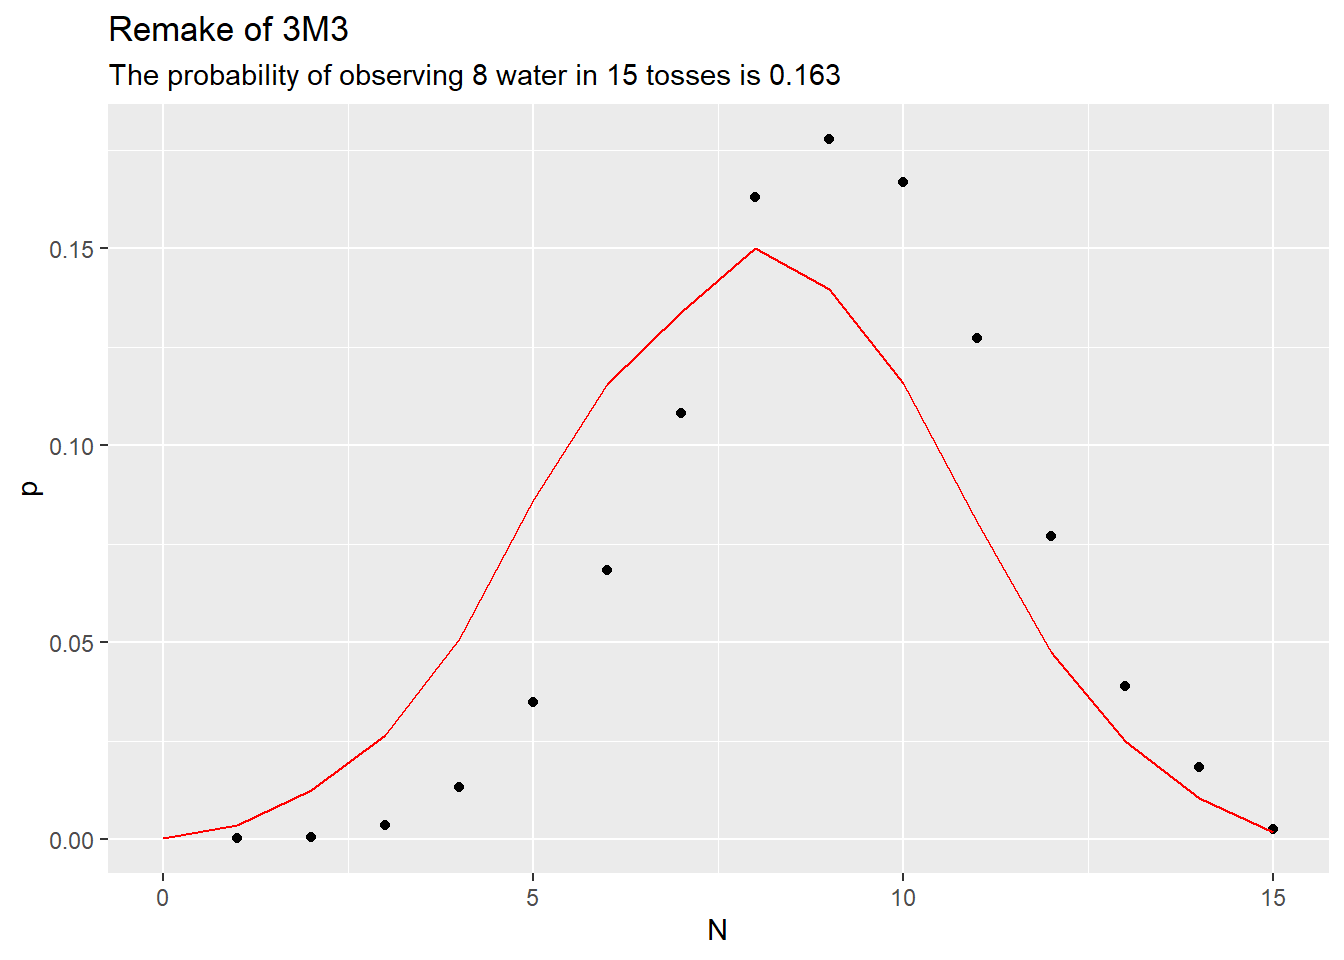
\includegraphics{notes-on-statistical-rethinking_files/figure-latex/3M5-3-1.pdf}

\begin{Shaded}
\begin{Highlighting}[]
\NormalTok{predicted\_water6\_}\DecValTok{9}\NormalTok{\_remake \textless{}{-}}\StringTok{ }
\StringTok{  }\KeywordTok{tibble}\NormalTok{(}\DataTypeTok{N =} \KeywordTok{rbinom}\NormalTok{(}\KeywordTok{length}\NormalTok{(samples), }\DataTypeTok{size=}\DecValTok{9}\NormalTok{, }\DataTypeTok{prob=}\NormalTok{samples)) }\OperatorTok{\%\textgreater{}\%}
\StringTok{  }\KeywordTok{group\_by}\NormalTok{(N) }\OperatorTok{\%\textgreater{}\%}
\StringTok{  }\KeywordTok{summarize}\NormalTok{(}\DataTypeTok{count =} \KeywordTok{n}\NormalTok{(), }\DataTypeTok{.groups =} \StringTok{\textquotesingle{}drop\textquotesingle{}}\NormalTok{)  }\OperatorTok{\%\textgreater{}\%}
\StringTok{  }\KeywordTok{ungroup}\NormalTok{() }\OperatorTok{\%\textgreater{}\%}
\StringTok{  }\KeywordTok{mutate}\NormalTok{(}\DataTypeTok{p =}\NormalTok{ count }\OperatorTok{/}\StringTok{ }\KeywordTok{sum}\NormalTok{(count))}
  
\NormalTok{p6 \textless{}{-}}\StringTok{ }
\StringTok{  }\NormalTok{predicted\_water6\_}\DecValTok{9}\NormalTok{\_remake }\OperatorTok{\%\textgreater{}\%}
\StringTok{  }\KeywordTok{filter}\NormalTok{(N }\OperatorTok{==}\StringTok{ }\DecValTok{6}\NormalTok{) }\OperatorTok{\%\textgreater{}\%}
\StringTok{  }\KeywordTok{pull}\NormalTok{(p)}

\KeywordTok{ggplot}\NormalTok{(predicted\_water6\_}\DecValTok{9}\NormalTok{\_remake, }\KeywordTok{aes}\NormalTok{(}\DataTypeTok{x=}\NormalTok{N, }\DataTypeTok{y=}\NormalTok{ p)) }\OperatorTok{+}\StringTok{ }
\StringTok{  }\KeywordTok{geom\_point}\NormalTok{() }\OperatorTok{+}\StringTok{ }
\StringTok{  }\KeywordTok{geom\_line}\NormalTok{(}\DataTypeTok{data=}\NormalTok{predicted\_water6\_}\DecValTok{9}\NormalTok{, }\DataTypeTok{color=}\StringTok{"red"}\NormalTok{) }\OperatorTok{+}
\StringTok{  }\KeywordTok{labs}\NormalTok{(}\DataTypeTok{subtitle =}\NormalTok{ glue}\OperatorTok{::}\KeywordTok{glue}\NormalTok{(}\StringTok{"The probability of observing 6 water in 9 tosses is \{p6\}"}\NormalTok{))}
\end{Highlighting}
\end{Shaded}

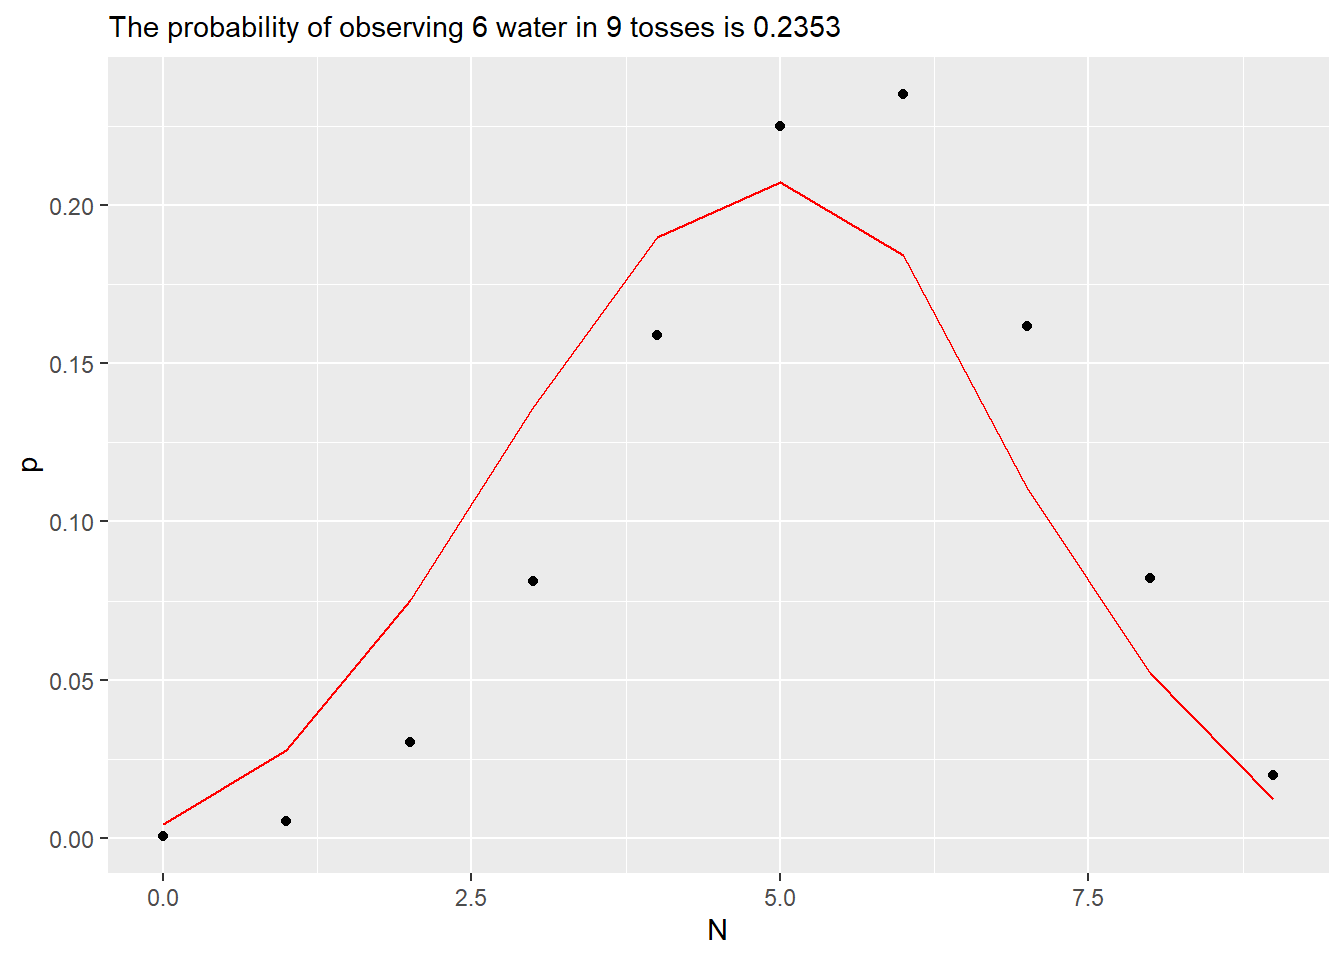
\includegraphics{notes-on-statistical-rethinking_files/figure-latex/3M5-4-1.pdf}

\hypertarget{m6-1}{%
\subsubsection*{3M6}\label{m6-1}}
\addcontentsline{toc}{subsubsection}{3M6}

Suppose you want to estimate the Earth's proportion of water very precisely. Specifically, you want the 99\% percentile interval of the posterior distribution of p to be only 0.05 wide. This means the distance between the upper and lower bound of the interval should be 0.05. How many times will you have to toss the globe to do this?

\begin{Shaded}
\begin{Highlighting}[]
\NormalTok{true\_proportion \textless{}{-}}\StringTok{ }\FloatTok{0.5}
\NormalTok{toss\_quantiles \textless{}{-}}\StringTok{ }
\StringTok{  }\KeywordTok{tibble}\NormalTok{(}\DataTypeTok{tossesN =} \KeywordTok{seq}\NormalTok{(}\DecValTok{10}\NormalTok{, }\DecValTok{3000}\NormalTok{, }\DataTypeTok{by=}\DecValTok{1}\NormalTok{)) }\OperatorTok{\%\textgreater{}\%}
\StringTok{  }\KeywordTok{mutate}\NormalTok{(}\DataTypeTok{lowerN =} \KeywordTok{qbinom}\NormalTok{(}\FloatTok{0.005}\NormalTok{, tossesN, true\_proportion),}
         \DataTypeTok{upperN =} \KeywordTok{qbinom}\NormalTok{(}\FloatTok{0.995}\NormalTok{, tossesN, true\_proportion),}
         \DataTypeTok{lowerP =}\NormalTok{ lowerN }\OperatorTok{/}\StringTok{ }\NormalTok{tossesN,}
         \DataTypeTok{upperP =}\NormalTok{ upperN }\OperatorTok{/}\StringTok{ }\NormalTok{tossesN,}
         \DataTypeTok{deltaP =}\NormalTok{ upperP }\OperatorTok{{-}}\StringTok{ }\NormalTok{lowerP)}

\NormalTok{minimal\_N \textless{}{-}}\StringTok{ }
\StringTok{  }\NormalTok{toss\_quantiles }\OperatorTok{\%\textgreater{}\%}
\StringTok{  }\KeywordTok{filter}\NormalTok{(deltaP }\OperatorTok{\textless{}}\StringTok{ }\FloatTok{0.05}\NormalTok{) }\OperatorTok{\%\textgreater{}\%}
\StringTok{  }\KeywordTok{slice}\NormalTok{(}\DecValTok{1}\NormalTok{) }\OperatorTok{\%\textgreater{}\%}
\StringTok{  }\KeywordTok{pull}\NormalTok{(tossesN)}

\KeywordTok{ggplot}\NormalTok{(toss\_quantiles, }\KeywordTok{aes}\NormalTok{(}\DataTypeTok{x=}\NormalTok{tossesN, }\DataTypeTok{y=}\NormalTok{deltaP)) }\OperatorTok{+}\StringTok{ }
\StringTok{  }\KeywordTok{geom\_line}\NormalTok{() }\OperatorTok{+}\StringTok{ }
\StringTok{  }\KeywordTok{geom\_hline}\NormalTok{(}\DataTypeTok{yintercept =} \FloatTok{0.05}\NormalTok{, }\DataTypeTok{color=}\StringTok{"red"}\NormalTok{) }\OperatorTok{+}\StringTok{ }
\StringTok{  }\KeywordTok{scale\_y\_log10}\NormalTok{() }\OperatorTok{+}\StringTok{ }
\StringTok{  }\KeywordTok{labs}\NormalTok{(}\DataTypeTok{title =} \StringTok{"Via qbinom"}\NormalTok{,}
       \DataTypeTok{subtitle =}\NormalTok{ glue}\OperatorTok{::}\KeywordTok{glue}\NormalTok{(}\StringTok{"For proportion \{true\_proportion\} you need \{minimal\_N\} tosses to get 99\% PI under 0.05"}\NormalTok{))}
\end{Highlighting}
\end{Shaded}

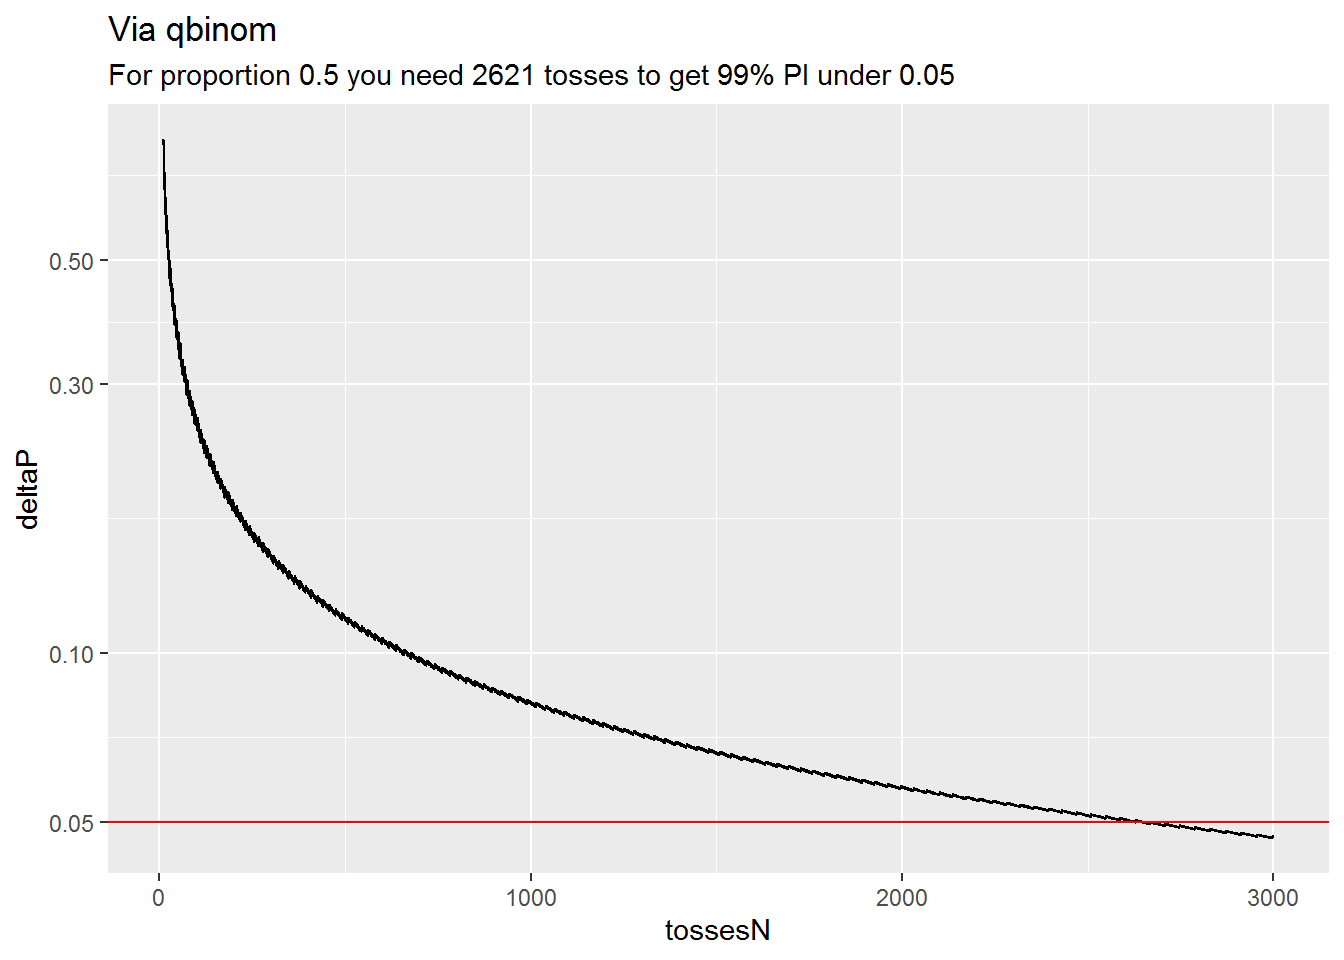
\includegraphics{notes-on-statistical-rethinking_files/figure-latex/3M6-qbinom-1.pdf}

\begin{Shaded}
\begin{Highlighting}[]
\NormalTok{simulate\_and\_compute\_PI99 \textless{}{-}}\StringTok{ }\ControlFlowTok{function}\NormalTok{(tossN, true\_proportion)\{}
\NormalTok{  simulated\_N \textless{}{-}}\StringTok{ }\KeywordTok{rbinom}\NormalTok{(}\FloatTok{1e4}\NormalTok{, tossN, true\_proportion)}
\NormalTok{  simulated\_P \textless{}{-}}\StringTok{ }\NormalTok{simulated\_N }\OperatorTok{/}\StringTok{ }\NormalTok{tossN}
  \KeywordTok{diff}\NormalTok{(rethinking}\OperatorTok{::}\KeywordTok{PI}\NormalTok{(simulated\_P, }\DataTypeTok{prob=}\FloatTok{0.99}\NormalTok{))}
\NormalTok{\}}

\NormalTok{true\_proportion \textless{}{-}}\StringTok{ }\FloatTok{0.5}
\NormalTok{toss\_sims \textless{}{-}}\StringTok{ }
\StringTok{  }\KeywordTok{tibble}\NormalTok{(}\DataTypeTok{tossesN =} \KeywordTok{seq}\NormalTok{(}\DecValTok{10}\NormalTok{, }\DecValTok{3000}\NormalTok{, }\DataTypeTok{by=}\DecValTok{1}\NormalTok{)) }\OperatorTok{\%\textgreater{}\%}
\StringTok{  }\KeywordTok{rowwise}\NormalTok{() }\OperatorTok{\%\textgreater{}\%}
\StringTok{  }\KeywordTok{mutate}\NormalTok{(}\DataTypeTok{deltaP =}\KeywordTok{simulate\_and\_compute\_PI99}\NormalTok{(tossesN, true\_proportion))}

\NormalTok{minimal\_N \textless{}{-}}\StringTok{ }
\StringTok{  }\NormalTok{toss\_sims }\OperatorTok{\%\textgreater{}\%}
\StringTok{  }\KeywordTok{filter}\NormalTok{(deltaP }\OperatorTok{\textless{}}\StringTok{ }\FloatTok{0.05}\NormalTok{) }\OperatorTok{\%\textgreater{}\%}
\StringTok{  }\KeywordTok{slice}\NormalTok{(}\DecValTok{1}\NormalTok{) }\OperatorTok{\%\textgreater{}\%}
\StringTok{  }\KeywordTok{pull}\NormalTok{(tossesN)}

\KeywordTok{ggplot}\NormalTok{(toss\_sims, }\KeywordTok{aes}\NormalTok{(}\DataTypeTok{x=}\NormalTok{tossesN, }\DataTypeTok{y=}\NormalTok{deltaP)) }\OperatorTok{+}\StringTok{ }
\StringTok{  }\KeywordTok{geom\_line}\NormalTok{() }\OperatorTok{+}\StringTok{ }
\StringTok{  }\KeywordTok{geom\_hline}\NormalTok{(}\DataTypeTok{yintercept =} \FloatTok{0.05}\NormalTok{, }\DataTypeTok{color=}\StringTok{"red"}\NormalTok{) }\OperatorTok{+}\StringTok{ }
\StringTok{  }\KeywordTok{scale\_y\_log10}\NormalTok{() }\OperatorTok{+}\StringTok{ }
\StringTok{  }\KeywordTok{labs}\NormalTok{(}\DataTypeTok{title =} \StringTok{"Via rbinom simulations"}\NormalTok{,}
       \DataTypeTok{subtitle =}\NormalTok{ glue}\OperatorTok{::}\KeywordTok{glue}\NormalTok{(}\StringTok{"For proportion \{true\_proportion\} you need \{minimal\_N\} tosses to get 99\% PI under 0.05"}\NormalTok{))}
\end{Highlighting}
\end{Shaded}

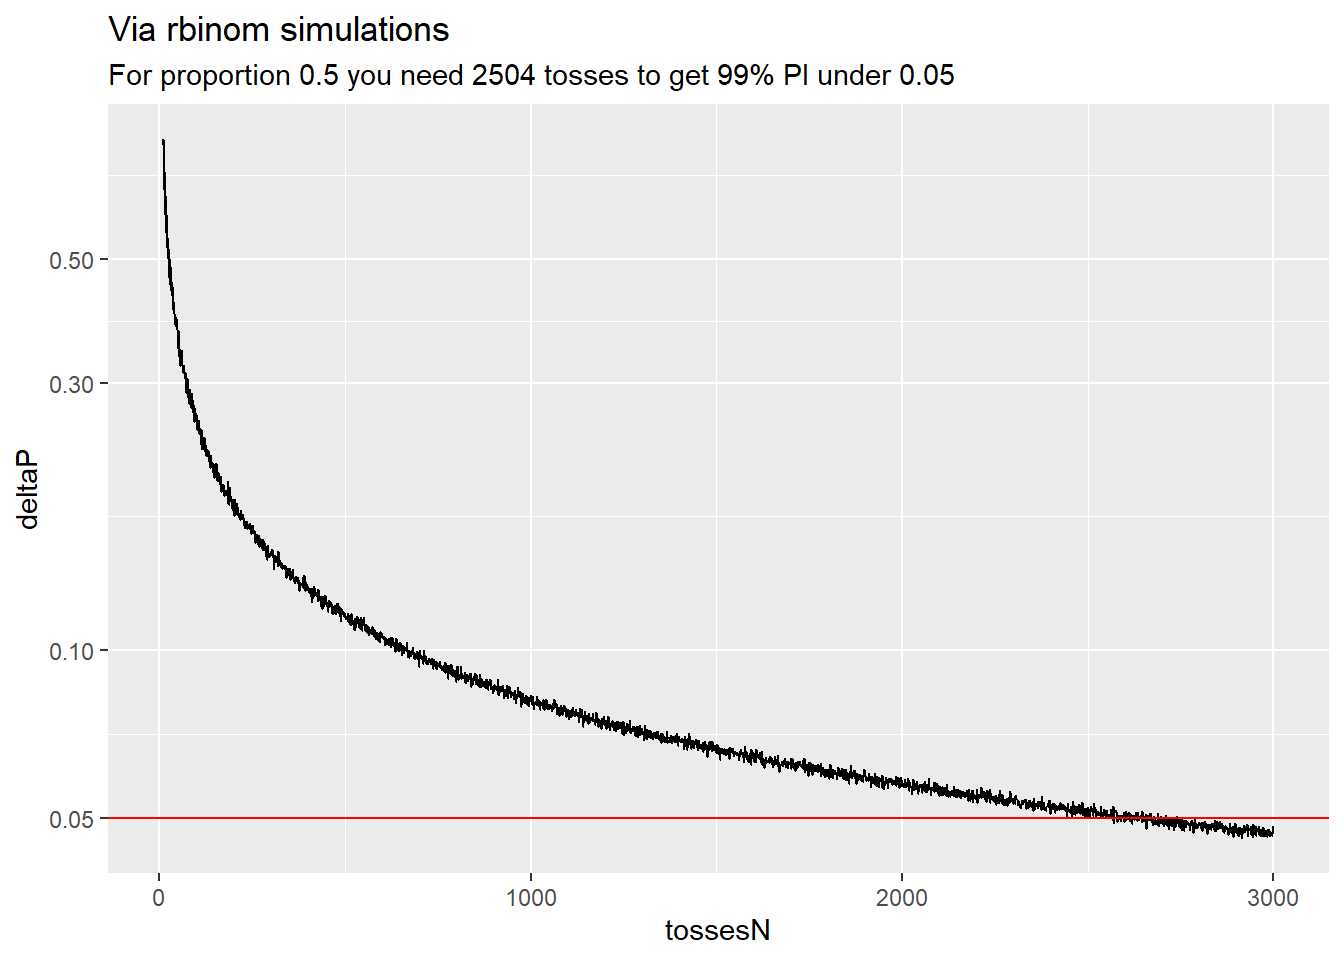
\includegraphics{notes-on-statistical-rethinking_files/figure-latex/3M6-simulation-1.pdf}

\hypertarget{hard}{%
\subsubsection*{Hard}\label{hard}}
\addcontentsline{toc}{subsubsection}{Hard}

\begin{Shaded}
\begin{Highlighting}[]
\KeywordTok{data}\NormalTok{(homeworkch3)}
\end{Highlighting}
\end{Shaded}

\hypertarget{h1-1}{%
\subsubsection*{3H1}\label{h1-1}}
\addcontentsline{toc}{subsubsection}{3H1}

Using grid approximation, compute the posterior distribution for the probability of a birth being a boy. Assume a uniform prior probability. Which parameter value maximizes the posterior probability?

\begin{Shaded}
\begin{Highlighting}[]
\NormalTok{birth \textless{}{-}}\StringTok{ }\KeywordTok{c}\NormalTok{(birth1, birth2)}
\NormalTok{birthN \textless{}{-}}\StringTok{ }\KeywordTok{length}\NormalTok{(birth)}
\NormalTok{boyN \textless{}{-}}\StringTok{ }\KeywordTok{sum}\NormalTok{(birth)}

\NormalTok{p\_grid \textless{}{-}}\StringTok{ }\KeywordTok{seq}\NormalTok{(}\DataTypeTok{from=}\DecValTok{0}\NormalTok{, }\DataTypeTok{to=}\DecValTok{1}\NormalTok{, }\DataTypeTok{length.out=}\DecValTok{1000}\NormalTok{)}
\NormalTok{prior \textless{}{-}}\StringTok{ }\KeywordTok{rep}\NormalTok{(}\DecValTok{1}\NormalTok{,}\DecValTok{1000}\NormalTok{)}
\NormalTok{likelihood \textless{}{-}}\StringTok{ }\KeywordTok{dbinom}\NormalTok{(boyN, }\DataTypeTok{size=}\NormalTok{birthN, }\DataTypeTok{prob=}\NormalTok{p\_grid)}
\NormalTok{posterior \textless{}{-}}\StringTok{ }\NormalTok{likelihood }\OperatorTok{*}\StringTok{ }\NormalTok{prior}
\NormalTok{posterior \textless{}{-}}\StringTok{ }\NormalTok{posterior }\OperatorTok{/}\StringTok{ }\KeywordTok{sum}\NormalTok{(posterior)}

\NormalTok{boyP \textless{}{-}}\StringTok{ }\NormalTok{p\_grid[}\KeywordTok{which.max}\NormalTok{(posterior)]}

\KeywordTok{ggplot}\NormalTok{(}\DataTypeTok{data=}\OtherTok{NULL}\NormalTok{, }\KeywordTok{aes}\NormalTok{(}\DataTypeTok{x=}\NormalTok{p\_grid, }\DataTypeTok{y=}\NormalTok{posterior)) }\OperatorTok{+}\StringTok{ }
\StringTok{  }\KeywordTok{geom\_line}\NormalTok{()}\OperatorTok{+}
\StringTok{  }\KeywordTok{geom\_vline}\NormalTok{(}\DataTypeTok{xintercept =}\NormalTok{ boyP, }\DataTypeTok{color=}\StringTok{"red"}\NormalTok{) }\OperatorTok{+}\StringTok{ }
\StringTok{  }\KeywordTok{labs}\NormalTok{(}\DataTypeTok{subtitle =}\NormalTok{ glue}\OperatorTok{::}\KeywordTok{glue}\NormalTok{(}\StringTok{"Mode: \{round(boyP, 3)\}"}\NormalTok{))}
\end{Highlighting}
\end{Shaded}

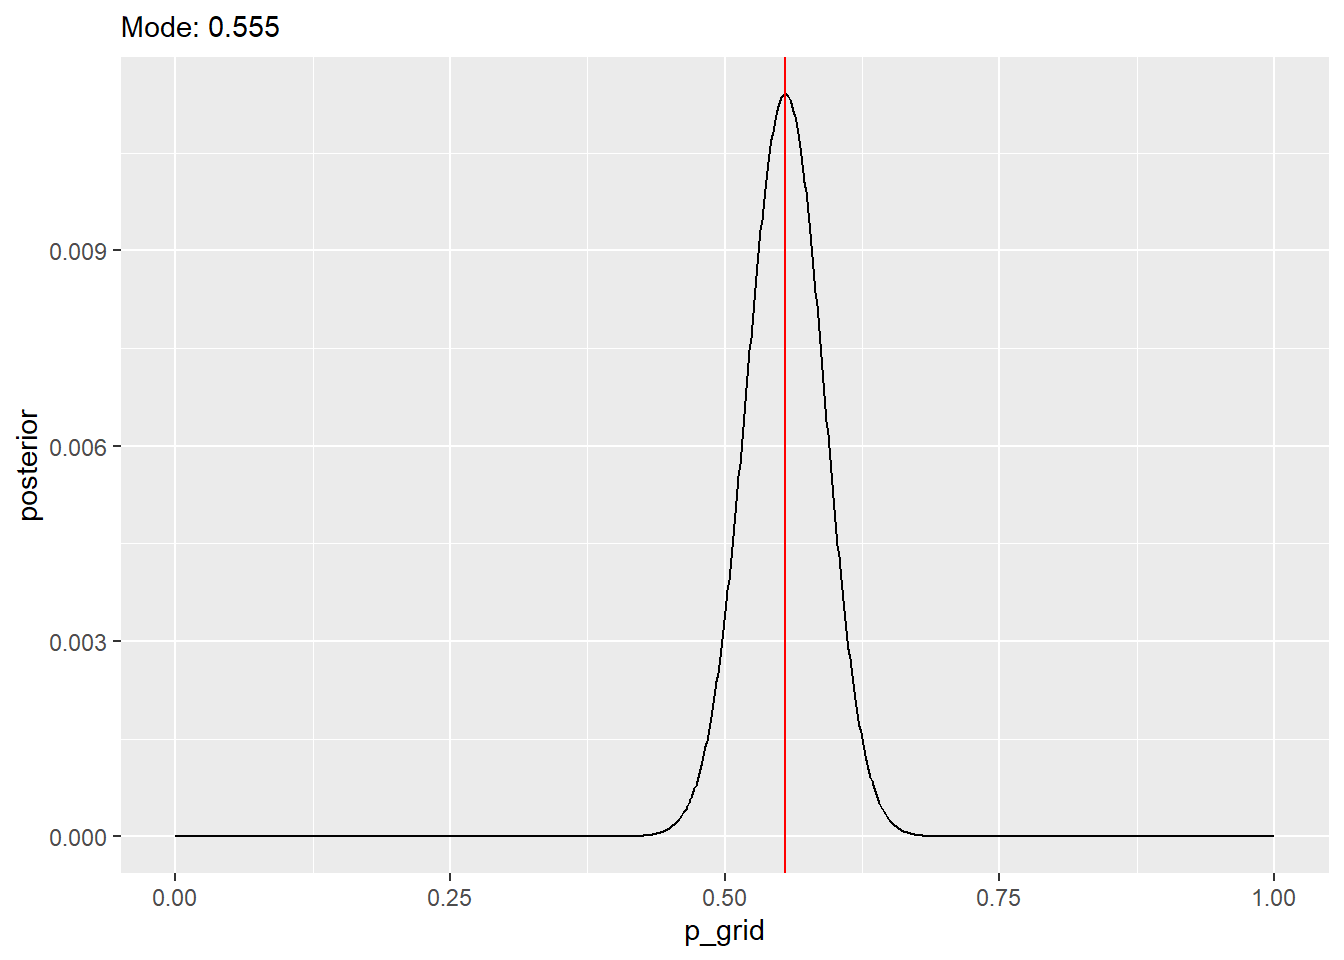
\includegraphics{notes-on-statistical-rethinking_files/figure-latex/3H1-1.pdf}

\hypertarget{h2-1}{%
\subsubsection*{3H2}\label{h2-1}}
\addcontentsline{toc}{subsubsection}{3H2}

Using the sample function, draw 10,000 random parameter values from the posterior distribution you calculated above. Use these samples to estimate the 50\%, 89\%, and 97\% highest posterior density intervals.

\begin{Shaded}
\begin{Highlighting}[]
\KeywordTok{set.seed}\NormalTok{(}\DecValTok{100}\NormalTok{)}
\NormalTok{samples \textless{}{-}}\StringTok{ }\KeywordTok{sample}\NormalTok{(p\_grid, }\DataTypeTok{prob=}\NormalTok{posterior, }\DataTypeTok{size=}\FloatTok{1e4}\NormalTok{, }\DataTypeTok{replace=}\OtherTok{TRUE}\NormalTok{)}

\NormalTok{HPDI50 \textless{}{-}}\StringTok{ }\NormalTok{rethinking}\OperatorTok{::}\KeywordTok{HPDI}\NormalTok{(samples, }\DataTypeTok{prob =} \FloatTok{0.5}\NormalTok{)}
\NormalTok{HPDI89 \textless{}{-}}\StringTok{ }\NormalTok{rethinking}\OperatorTok{::}\KeywordTok{HPDI}\NormalTok{(samples, }\DataTypeTok{prob =} \FloatTok{0.89}\NormalTok{)}
\NormalTok{HPDI97 \textless{}{-}}\StringTok{ }\NormalTok{rethinking}\OperatorTok{::}\KeywordTok{HPDI}\NormalTok{(samples, }\DataTypeTok{prob =} \FloatTok{0.97}\NormalTok{)}

\NormalTok{all\_HPDI \textless{}{-}}\StringTok{ }\KeywordTok{c}\NormalTok{(HPDI50, HPDI89, HPDI97)}
\KeywordTok{names}\NormalTok{(all\_HPDI) \textless{}{-}}\StringTok{ }\OtherTok{NULL}


\KeywordTok{ggplot}\NormalTok{(}\DataTypeTok{data=}\OtherTok{NULL}\NormalTok{, }\KeywordTok{aes}\NormalTok{(}\DataTypeTok{x=}\NormalTok{samples)) }\OperatorTok{+}\StringTok{ }
\StringTok{  }\KeywordTok{geom\_histogram}\NormalTok{(}\DataTypeTok{bins=}\DecValTok{40}\NormalTok{) }\OperatorTok{+}\StringTok{ }
\StringTok{  }\KeywordTok{geom\_vline}\NormalTok{(}\DataTypeTok{xintercept =}\NormalTok{ HPDI50, }\DataTypeTok{color=}\StringTok{"green"}\NormalTok{) }\OperatorTok{+}
\StringTok{  }\KeywordTok{geom\_vline}\NormalTok{(}\DataTypeTok{xintercept =}\NormalTok{ HPDI89, }\DataTypeTok{color=}\StringTok{"blue"}\NormalTok{) }\OperatorTok{+}\StringTok{ }
\StringTok{  }\KeywordTok{geom\_vline}\NormalTok{(}\DataTypeTok{xintercept =}\NormalTok{ HPDI97, }\DataTypeTok{color=}\StringTok{"red"}\NormalTok{) }\OperatorTok{+}
\StringTok{  }\KeywordTok{scale\_x\_continuous}\NormalTok{(}\DataTypeTok{breaks =}\NormalTok{ all\_HPDI, }\DataTypeTok{labels =} \KeywordTok{round}\NormalTok{(all\_HPDI, }\DecValTok{3}\NormalTok{))}
\end{Highlighting}
\end{Shaded}

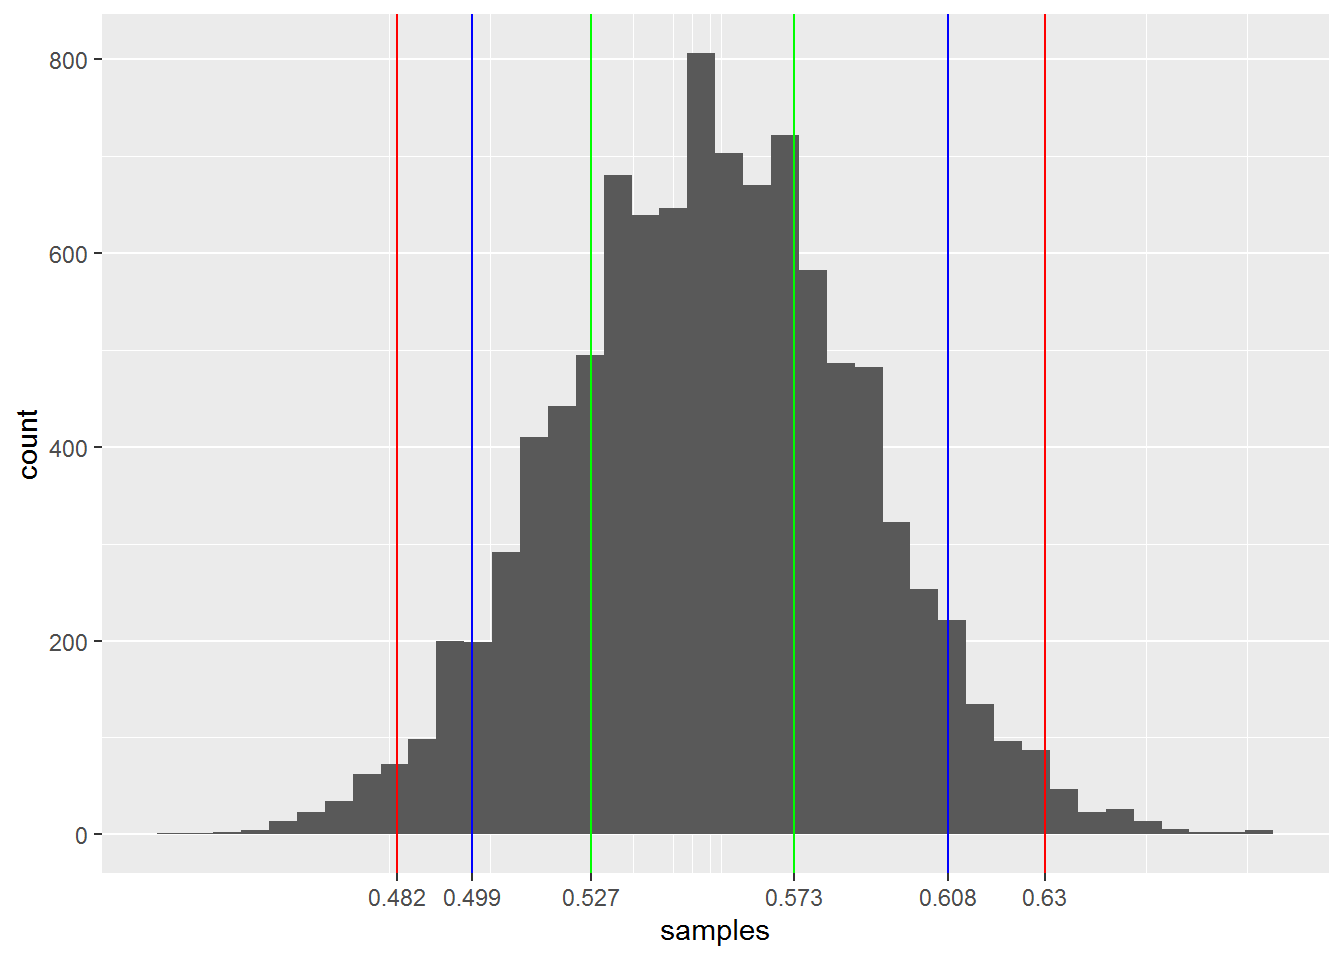
\includegraphics{notes-on-statistical-rethinking_files/figure-latex/3H2-1.pdf}

\hypertarget{h3-1}{%
\subsubsection*{3H3}\label{h3-1}}
\addcontentsline{toc}{subsubsection}{3H3}

Use rbinom to simulate 10,000 replicates of 200 births. You should end up with 10,000 numbers, each one a count of boys out of 200 births. Compare the distribution of predicted numbers of boys to the actual count in the data (111 boys out of 200 births). There are many good ways to visualize the simulations, but the dens command (part of the rethinking package) is probably the easiest way in this case. Does it look like the model fits the data well? That is, does the distribution of predictions include the actual observation as a central, likely outcome?

\begin{Shaded}
\begin{Highlighting}[]
\NormalTok{sim\_boys \textless{}{-}}\StringTok{ }\KeywordTok{rbinom}\NormalTok{(}\FloatTok{1e4}\NormalTok{, }\DecValTok{200}\NormalTok{, boyN }\OperatorTok{/}\StringTok{ }\NormalTok{birthN)}

\KeywordTok{ggplot}\NormalTok{(}\DataTypeTok{data=}\OtherTok{NULL}\NormalTok{, }\KeywordTok{aes}\NormalTok{(}\DataTypeTok{x=}\NormalTok{sim\_boys)) }\OperatorTok{+}\StringTok{ }
\StringTok{  }\KeywordTok{geom\_density}\NormalTok{() }\OperatorTok{+}\StringTok{ }
\StringTok{  }\KeywordTok{geom\_vline}\NormalTok{(}\DataTypeTok{xintercept =}\NormalTok{ boyN, }\DataTypeTok{color=}\StringTok{"red"}\NormalTok{)}
\end{Highlighting}
\end{Shaded}

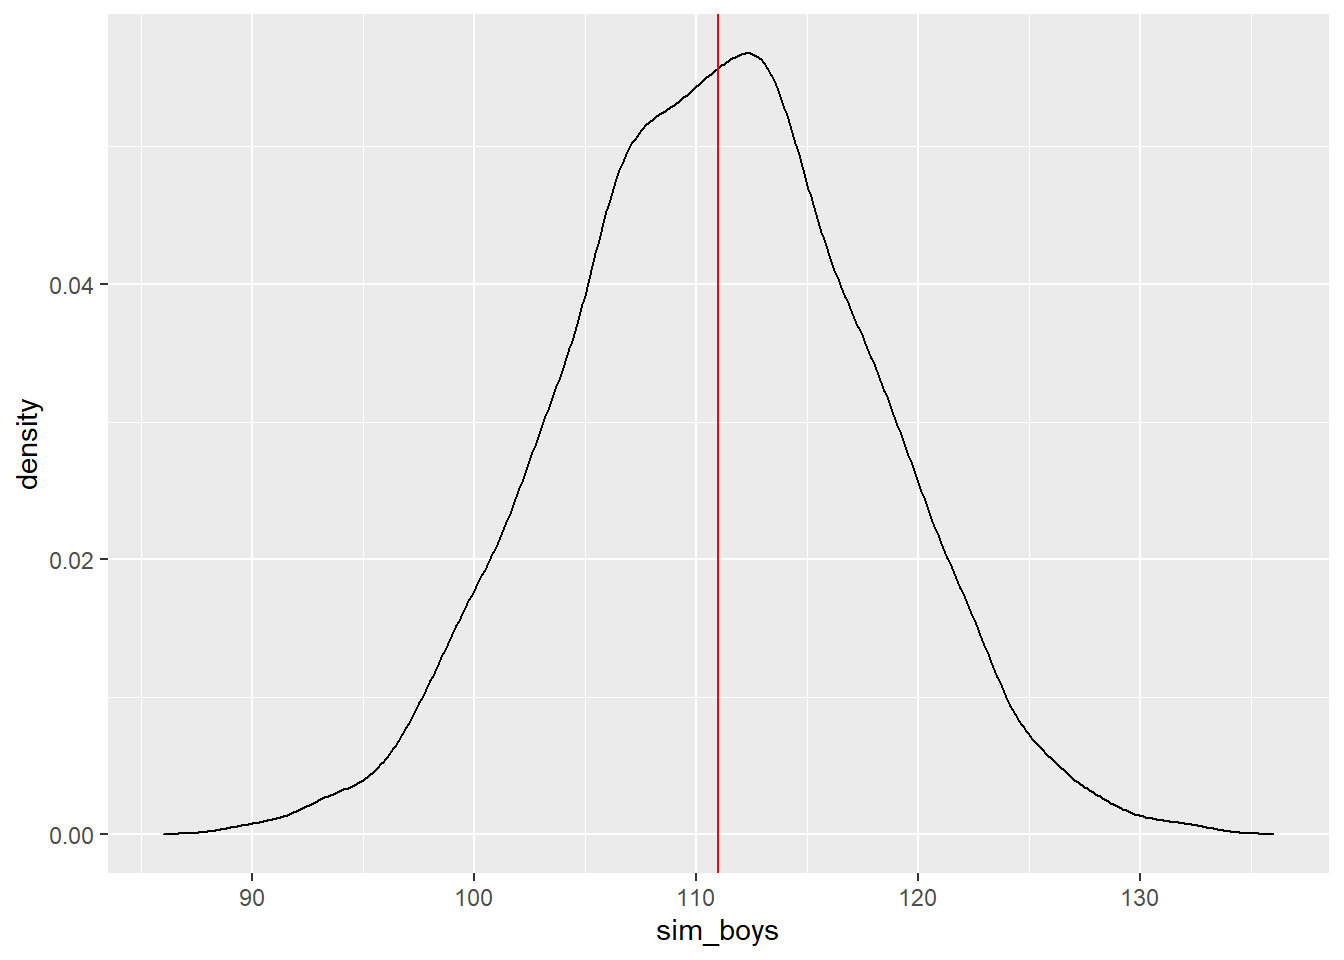
\includegraphics{notes-on-statistical-rethinking_files/figure-latex/3H3-1.pdf}

\hypertarget{h4-1}{%
\subsubsection*{3H4}\label{h4-1}}
\addcontentsline{toc}{subsubsection}{3H4}

Now compare 10,000 counts of boys from 100 simulated first borns only to the number of boys in the first births, birth1. How does the model look in this light?

\begin{Shaded}
\begin{Highlighting}[]
\NormalTok{sim\_boys \textless{}{-}}\StringTok{ }\KeywordTok{rbinom}\NormalTok{(}\FloatTok{1e4}\NormalTok{, }\DecValTok{100}\NormalTok{, boyN }\OperatorTok{/}\StringTok{ }\NormalTok{birthN)}

\KeywordTok{ggplot}\NormalTok{(}\DataTypeTok{data=}\OtherTok{NULL}\NormalTok{, }\KeywordTok{aes}\NormalTok{(}\DataTypeTok{x=}\NormalTok{sim\_boys)) }\OperatorTok{+}\StringTok{ }
\StringTok{  }\KeywordTok{geom\_density}\NormalTok{() }\OperatorTok{+}\StringTok{ }
\StringTok{  }\KeywordTok{geom\_vline}\NormalTok{(}\DataTypeTok{xintercept =} \KeywordTok{sum}\NormalTok{(birth1), }\DataTypeTok{color=}\StringTok{"red"}\NormalTok{)}
\end{Highlighting}
\end{Shaded}

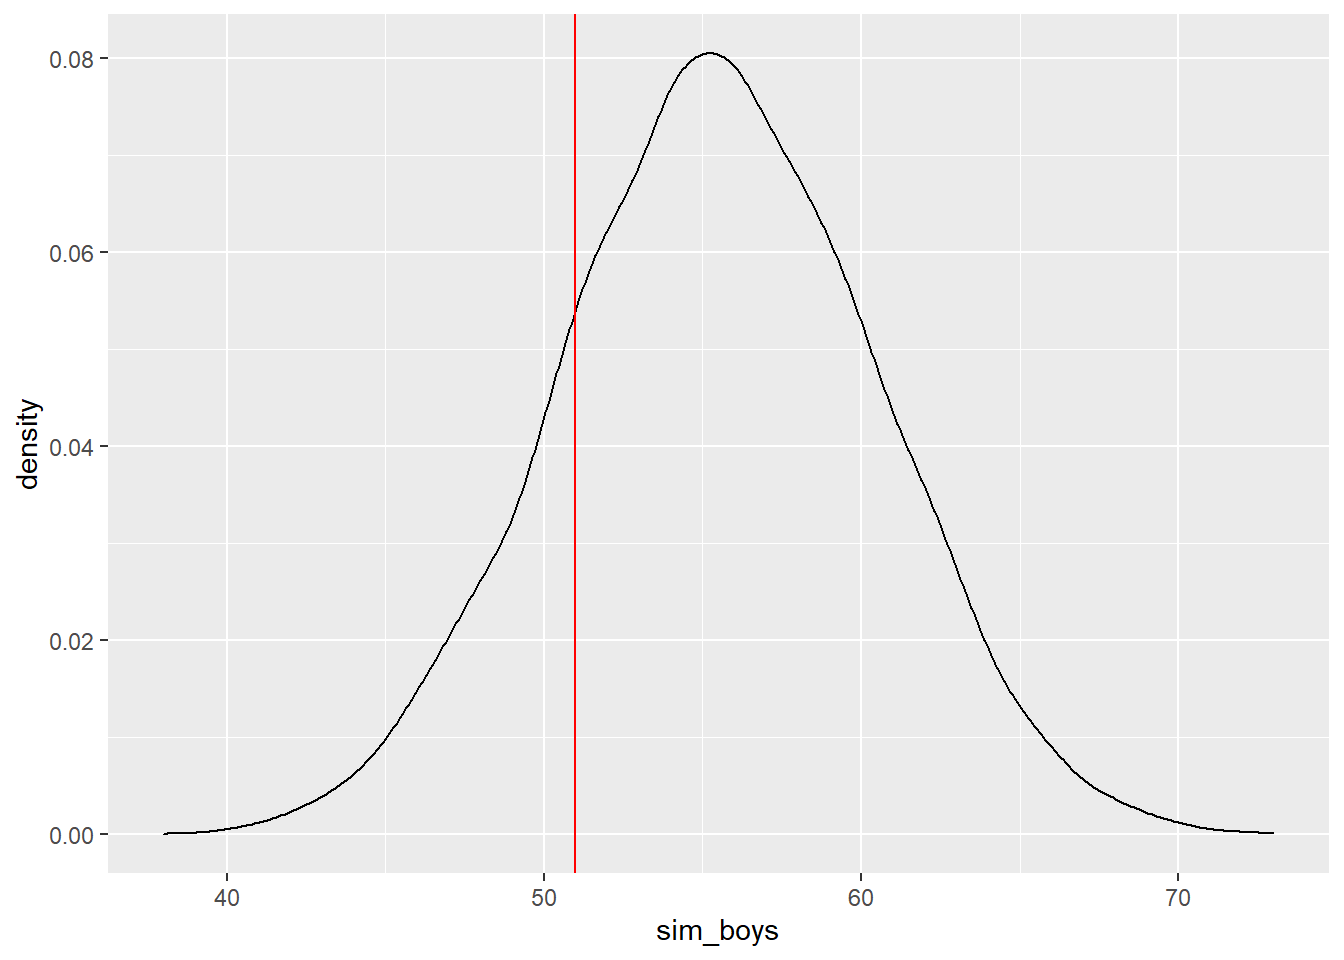
\includegraphics{notes-on-statistical-rethinking_files/figure-latex/3H4-1.pdf}

\hypertarget{h5}{%
\subsubsection*{3H5}\label{h5}}
\addcontentsline{toc}{subsubsection}{3H5}

The model assumes that sex of first and second births are independent. To check this assumption, focus now on second births that followed female first borns. Compare 10,000 simulated counts of boys to only those second births that followed girls. To do this correctly, you need to count the number of first borns who were girls and simulate that many births, 10,000 times. Compare the counts of boys in your simulations to the actual observed count of boys following girls. How does the model look in this light? Any guesses what is going on in these data?

\begin{Shaded}
\begin{Highlighting}[]
\NormalTok{birth\_after\_girl \textless{}{-}}\StringTok{ }\NormalTok{birth2[birth1 }\OperatorTok{==}\StringTok{ }\DecValTok{0}\NormalTok{]}
\NormalTok{sim\_boys \textless{}{-}}\StringTok{ }\KeywordTok{rbinom}\NormalTok{(}\FloatTok{1e4}\NormalTok{, }\KeywordTok{length}\NormalTok{(birth\_after\_girl), boyN }\OperatorTok{/}\StringTok{ }\NormalTok{birthN)}

\KeywordTok{ggplot}\NormalTok{(}\DataTypeTok{data=}\OtherTok{NULL}\NormalTok{, }\KeywordTok{aes}\NormalTok{(}\DataTypeTok{x=}\NormalTok{sim\_boys)) }\OperatorTok{+}\StringTok{ }
\StringTok{  }\KeywordTok{geom\_density}\NormalTok{() }\OperatorTok{+}\StringTok{ }
\StringTok{  }\KeywordTok{geom\_vline}\NormalTok{(}\DataTypeTok{xintercept =} \KeywordTok{sum}\NormalTok{(birth\_after\_girl), }\DataTypeTok{color=}\StringTok{"red"}\NormalTok{)}
\end{Highlighting}
\end{Shaded}

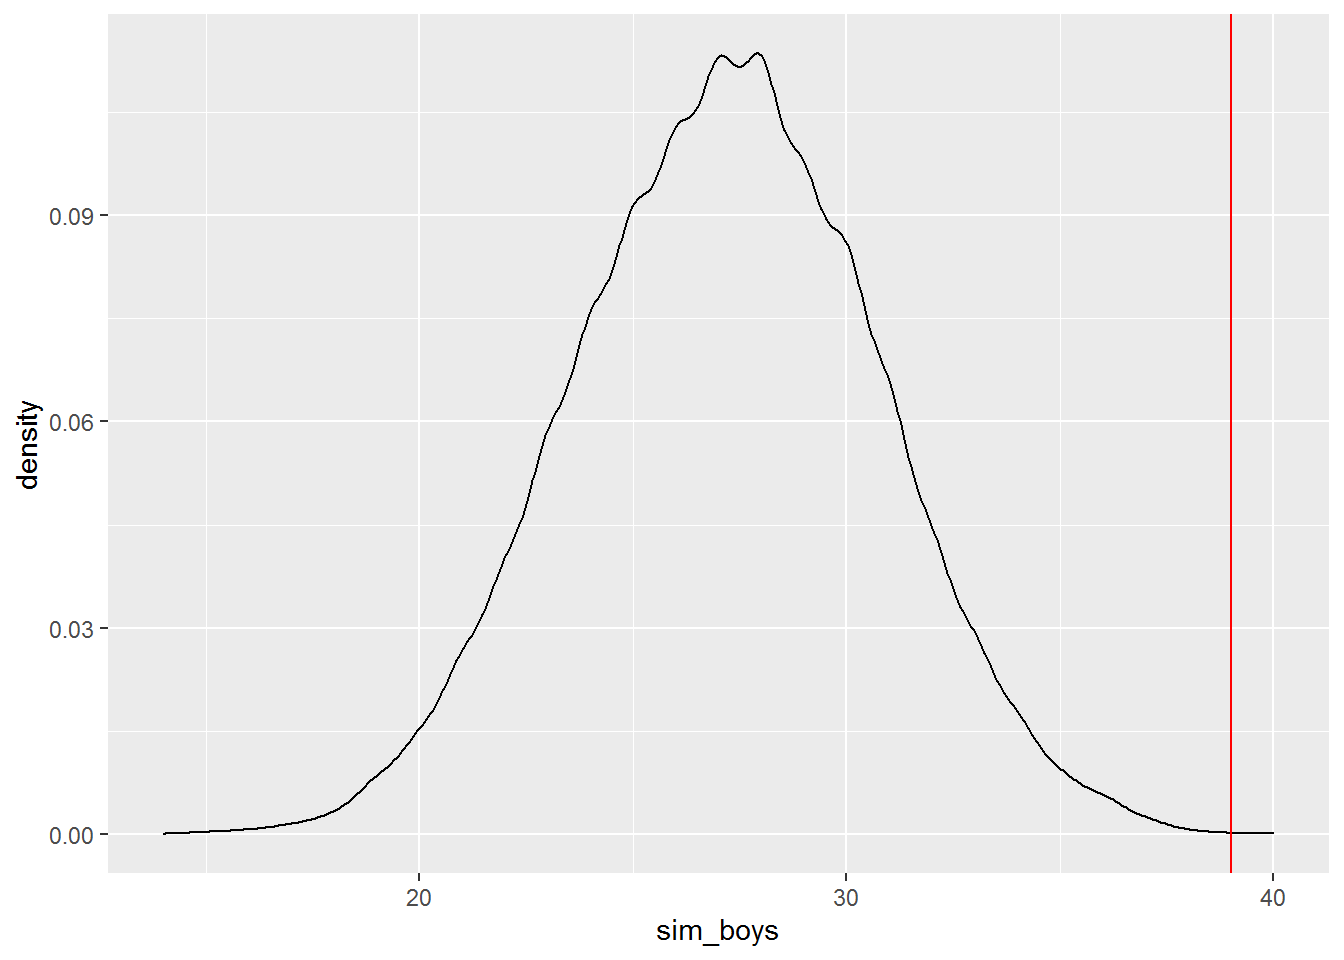
\includegraphics{notes-on-statistical-rethinking_files/figure-latex/3H5-1.pdf}

\hypertarget{solutions-for-chapter-4}{%
\chapter{Solutions for Chapter 4}\label{solutions-for-chapter-4}}

\hypertarget{e1-2}{%
\subsubsection*{4E1}\label{e1-2}}
\addcontentsline{toc}{subsubsection}{4E1}

In the model definition below, which line is the likelihood?
\[\rightarrow ~ y_i \sim Normal(\mu, \sigma) ~ \leftarrow\\
\mu \sim Normal(0, 10) \\
\sigma \sim Exponential(1)\]

\hypertarget{e2-2}{%
\subsubsection*{4E2}\label{e2-2}}
\addcontentsline{toc}{subsubsection}{4E2}

In the model definition just above, how many parameters are in the posterior distribution?

**Two: \(\mu\) and \(\sigma\).

\hypertarget{e3-2}{%
\subsubsection*{4E3}\label{e3-2}}
\addcontentsline{toc}{subsubsection}{4E3}

Using the model definition above, write down the appropriate form of Bayes' theorem that includes the proper likelihood and priors.

\[
Pr(\mu, \sigma | y) = \frac{\prod_i Normal(y_i| \mu, \sigma) \cdot Normal(mu | 0, 10) \cdot Exponential(\sigma | 1)}
{\int \int \prod_i Normal(y_i| \mu, \sigma) \cdot Normal(mu | 0, 10) \cdot Exponential(\sigma | 1) \partial \mu \partial \sigma}
\]

\hypertarget{e4-2}{%
\subsubsection*{4E4}\label{e4-2}}
\addcontentsline{toc}{subsubsection}{4E4}

In the model definition below, which line is the linear model?

\[y_i ∼ Normal(\mu, \sigma) \\
\rightarrow ~\mu_i = \alpha + \beta x_i ~\leftarrow\\
α ∼ Normal(0, 10) \\ 
β ∼ Normal(0, 1) \\
σ ∼ Exponential(2)\]

\hypertarget{e5-1}{%
\subsubsection*{4E5}\label{e5-1}}
\addcontentsline{toc}{subsubsection}{4E5}

In the model definition just above, how many parameters are in the posterior distribution?

Three, \(α\), \(β\) (used to compute \(\mu\)), and \(\sigma\).

\hypertarget{m1-2}{%
\subsubsection*{4M1}\label{m1-2}}
\addcontentsline{toc}{subsubsection}{4M1}

For the model definition below, simulate observed y values from the prior (not the posterior).

\[y_i \sim Normal(\mu,\sigma) \\
\mu \sim Normal(0, 10) \\
\sigma \sim Exponential(1)\]

\begin{Shaded}
\begin{Highlighting}[]
\KeywordTok{library}\NormalTok{(ggplot2)}

\NormalTok{samples\_N \textless{}{-}}\StringTok{ }\FloatTok{1e4}
\NormalTok{mu \textless{}{-}}\StringTok{ }\KeywordTok{rnorm}\NormalTok{(samples\_N, }\DecValTok{0}\NormalTok{, }\DecValTok{10}\NormalTok{)}
\NormalTok{sigma \textless{}{-}}\StringTok{ }\KeywordTok{rexp}\NormalTok{(samples\_N, }\DecValTok{1}\NormalTok{)}
\NormalTok{y\_sim \textless{}{-}}\StringTok{ }\KeywordTok{rnorm}\NormalTok{(samples\_N, mu, sigma)}

\KeywordTok{ggplot}\NormalTok{(}\DataTypeTok{data=}\OtherTok{NULL}\NormalTok{, }\KeywordTok{aes}\NormalTok{(}\DataTypeTok{x=}\NormalTok{y\_sim)) }\OperatorTok{+}\StringTok{ }
\StringTok{  }\KeywordTok{geom\_histogram}\NormalTok{(}\DataTypeTok{bins=}\DecValTok{50}\NormalTok{) }\OperatorTok{+}\StringTok{ }
\StringTok{  }\KeywordTok{xlab}\NormalTok{(}\StringTok{"Simulated Y"}\NormalTok{)}
\end{Highlighting}
\end{Shaded}

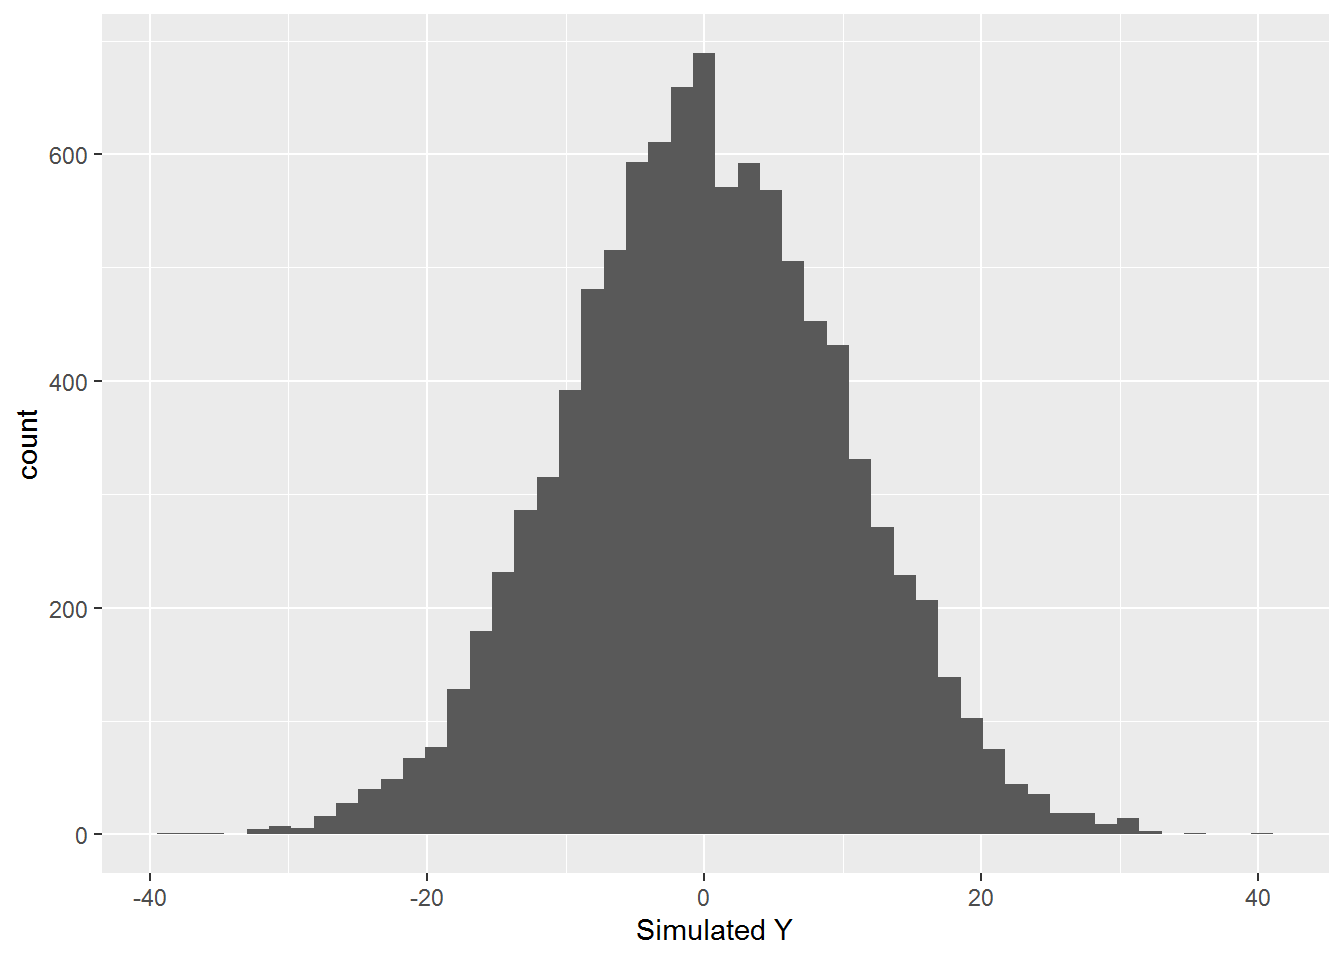
\includegraphics{notes-on-statistical-rethinking_files/figure-latex/4M1-1.pdf}

\hypertarget{m2-2}{%
\subsubsection*{4M2}\label{m2-2}}
\addcontentsline{toc}{subsubsection}{4M2}

Translate the model just above into a quap formula.

\begin{Shaded}
\begin{Highlighting}[]
\NormalTok{quap\_formula \textless{}{-}}\StringTok{ }\KeywordTok{alist}\NormalTok{(}
\NormalTok{  y }\OperatorTok{\textasciitilde{}}\StringTok{ }\KeywordTok{dnorm}\NormalTok{(mu, sigma),}
\NormalTok{  mu }\OperatorTok{\textasciitilde{}}\StringTok{ }\KeywordTok{dnorm}\NormalTok{(}\DecValTok{0}\NormalTok{,}\DecValTok{10}\NormalTok{),}
\NormalTok{  sigma }\OperatorTok{\textasciitilde{}}\StringTok{ }\KeywordTok{dexp}\NormalTok{(}\DecValTok{1}\NormalTok{))}
\end{Highlighting}
\end{Shaded}

\hypertarget{m3-2}{%
\subsubsection*{4M3}\label{m3-2}}
\addcontentsline{toc}{subsubsection}{4M3}

Translate the quap model formula below into a mathematical model definition.

\begin{verbatim}
y ~ dnorm( mu , sigma ),
mu <- a + b*x,
a ~ dnorm( 0 , 10 ),
b ~ dunif( 0 , 1 ),
sigma ~ dexp( 1 )
\end{verbatim}

\[y_i ∼ Normal(\mu, \sigma) \\
\mu_i = \alpha + \beta x_i \\
α ∼ Normal(0, 10) \\ 
β ∼ Uniform(0, 1) \\
σ ∼ Exponential(1)\]

\hypertarget{m4-2}{%
\subsubsection*{4M4}\label{m4-2}}
\addcontentsline{toc}{subsubsection}{4M4}

A sample of students is measured for height each year for 3 years. After the third year, you want to fit a linear regression predicting height using year as a predictor. Write down the mathematical model definition for this regression, using any variable names and priors you choose. Be prepared to defend your choice of priors.

I assume \emph{students} as in \emph{college students}. Therefore, you would expect an adult height, may be slightly lower, hence \texttt{170} for the intercept. You don't expect them to grow much, hence conservative slope for the effect of the year. I assume a fairly broad but strictly positive prior for \(\sigma\).

\[h_i ∼ Normal(\mu, \sigma) \\
\mu_i = \alpha + \beta year_i \\
α ∼ Normal(170, 10) \\ 
β ∼ Normal(0, 1) \\
σ ∼ Exponential(0.1)\]

\hypertarget{m5-2}{%
\subsubsection*{4M5}\label{m5-2}}
\addcontentsline{toc}{subsubsection}{4M5}

Now suppose I remind you that every student got taller each year. Does this information lead you to change your choice of priors? How?

I would ensure that \(\beta\) can be only positive, so \(β ∼ Exponential(1)\).

\hypertarget{m6-2}{%
\subsubsection*{4M6}\label{m6-2}}
\addcontentsline{toc}{subsubsection}{4M6}

Now suppose I tell you that the variance among heights for students of the same age is never more than 64cm. How does this lead you to revise your priors?

Based on the density plot, I would pick a more conservative prior of \(\sigma \sim Exponential(0.5)\) that drops off more rapidly and just barely includes \(\sqrt(64)\).

\begin{Shaded}
\begin{Highlighting}[]
\NormalTok{x \textless{}{-}}\StringTok{ }\KeywordTok{seq}\NormalTok{(}\DecValTok{0}\NormalTok{, }\DecValTok{10}\NormalTok{, }\DataTypeTok{length.out=}\DecValTok{100}\NormalTok{)}
\KeywordTok{ggplot}\NormalTok{(}\DataTypeTok{data=}\OtherTok{NULL}\NormalTok{, }\KeywordTok{aes}\NormalTok{(}\DataTypeTok{x=}\NormalTok{x, }\DataTypeTok{y=} \KeywordTok{dexp}\NormalTok{(x, }\FloatTok{0.5}\NormalTok{))) }\OperatorTok{+}\StringTok{ }
\StringTok{  }\KeywordTok{geom\_line}\NormalTok{() }\OperatorTok{+}
\StringTok{  }\KeywordTok{scale\_x\_continuous}\NormalTok{(}\DataTypeTok{breaks =} \DecValTok{0}\OperatorTok{:}\DecValTok{10}\NormalTok{) }\OperatorTok{+}
\StringTok{  }\KeywordTok{ylab}\NormalTok{(}\StringTok{"Probability density"}\NormalTok{)}
\end{Highlighting}
\end{Shaded}

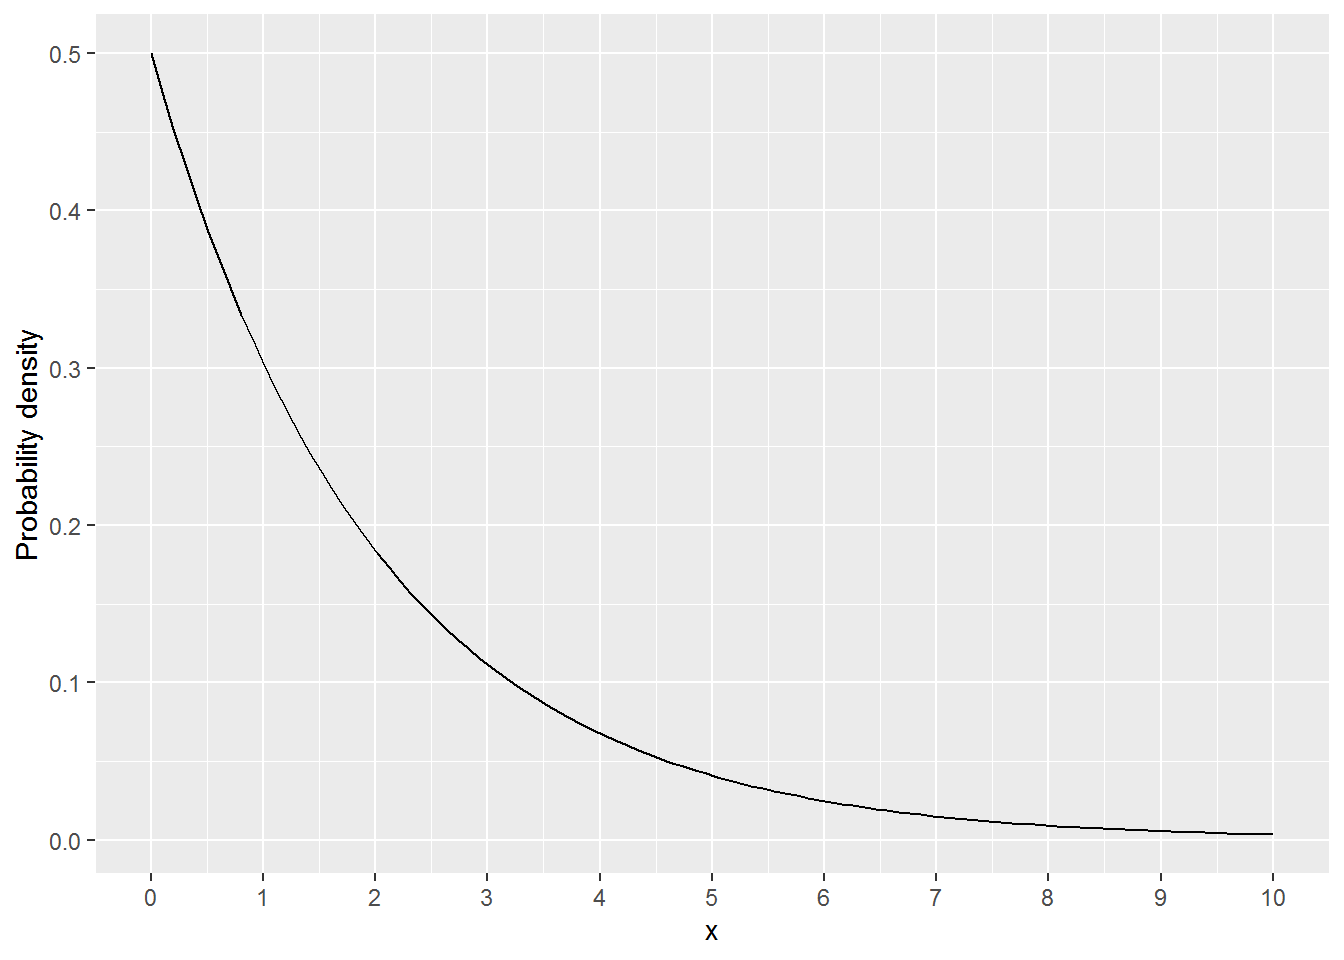
\includegraphics{notes-on-statistical-rethinking_files/figure-latex/unnamed-chunk-13-1.pdf}

\hypertarget{m7-1}{%
\subsubsection*{4M7}\label{m7-1}}
\addcontentsline{toc}{subsubsection}{4M7}

Refit model m4.3 from the chapter, but omit the mean weight xbar this time. Compare the new model's posterior to that of the original model. In particular, look at the covariance among the parameters. What is different? Then compare the posterior predictions of both models.

\begin{Shaded}
\begin{Highlighting}[]
\CommentTok{\# load data again, since it\textquotesingle{}s a long way back}
\KeywordTok{library}\NormalTok{(rethinking)}
\KeywordTok{data}\NormalTok{(Howell1); }
\NormalTok{d \textless{}{-}}\StringTok{ }\NormalTok{Howell1; }
\NormalTok{d2 \textless{}{-}}\StringTok{ }\NormalTok{d[d}\OperatorTok{$}\NormalTok{age }\OperatorTok{\textgreater{}=}\StringTok{ }\DecValTok{18}\NormalTok{,]}

\CommentTok{\# define the average weight, x{-}bar}
\NormalTok{xbar \textless{}{-}}\StringTok{ }\KeywordTok{mean}\NormalTok{(d2}\OperatorTok{$}\NormalTok{weight)}
\CommentTok{\# fit model}

\NormalTok{m4\_3c \textless{}{-}}\StringTok{ }\KeywordTok{quap}\NormalTok{(}
  \KeywordTok{alist}\NormalTok{(}
\NormalTok{    height }\OperatorTok{\textasciitilde{}}\StringTok{ }\KeywordTok{dnorm}\NormalTok{(mu, sigma),}
\NormalTok{    mu \textless{}{-}}\StringTok{ }\NormalTok{a }\OperatorTok{+}\StringTok{ }\NormalTok{b }\OperatorTok{*}\StringTok{ }\NormalTok{(weight }\OperatorTok{{-}}\StringTok{ }\NormalTok{xbar),}
\NormalTok{    a }\OperatorTok{\textasciitilde{}}\StringTok{ }\KeywordTok{dnorm}\NormalTok{(}\DecValTok{178}\NormalTok{, }\DecValTok{20}\NormalTok{) ,}
\NormalTok{    b }\OperatorTok{\textasciitilde{}}\StringTok{ }\KeywordTok{dlnorm}\NormalTok{(}\DecValTok{0}\NormalTok{, }\DecValTok{1}\NormalTok{) ,}
\NormalTok{    sigma }\OperatorTok{\textasciitilde{}}\StringTok{ }\KeywordTok{dunif}\NormalTok{(}\DecValTok{0}\NormalTok{, }\DecValTok{50}\NormalTok{)) , }
  \DataTypeTok{data=}\NormalTok{d2)}

\NormalTok{m4\_}\DecValTok{3}\NormalTok{ \textless{}{-}}\StringTok{ }\KeywordTok{quap}\NormalTok{(}
  \KeywordTok{alist}\NormalTok{(}
\NormalTok{    height }\OperatorTok{\textasciitilde{}}\StringTok{ }\KeywordTok{dnorm}\NormalTok{(mu, sigma),}
\NormalTok{    mu \textless{}{-}}\StringTok{ }\NormalTok{a }\OperatorTok{+}\StringTok{ }\NormalTok{b }\OperatorTok{*}\StringTok{ }\NormalTok{weight,}
\NormalTok{    a }\OperatorTok{\textasciitilde{}}\StringTok{ }\KeywordTok{dnorm}\NormalTok{(}\DecValTok{178}\NormalTok{, }\DecValTok{20}\NormalTok{) ,}
\NormalTok{    b }\OperatorTok{\textasciitilde{}}\StringTok{ }\KeywordTok{dlnorm}\NormalTok{(}\DecValTok{0}\NormalTok{, }\DecValTok{1}\NormalTok{) ,}
\NormalTok{    sigma }\OperatorTok{\textasciitilde{}}\StringTok{ }\KeywordTok{dunif}\NormalTok{(}\DecValTok{0}\NormalTok{, }\DecValTok{50}\NormalTok{)) , }
  \DataTypeTok{data=}\NormalTok{d2)}

\KeywordTok{precis}\NormalTok{(m4\_}\DecValTok{3}\NormalTok{)}
\end{Highlighting}
\end{Shaded}

\begin{verbatim}
##              mean         sd        5.5%       94.5%
## a     114.5342008 1.89774719 111.5012343 117.5671674
## b       0.8907326 0.04175799   0.8239952   0.9574699
## sigma   5.0727190 0.19124895   4.7670662   5.3783718
\end{verbatim}

\begin{Shaded}
\begin{Highlighting}[]
\KeywordTok{precis}\NormalTok{(m4\_3c)}
\end{Highlighting}
\end{Shaded}

\begin{verbatim}
##              mean         sd        5.5%      94.5%
## a     154.6013683 0.27030768 154.1693645 155.033372
## b       0.9032809 0.04192363   0.8362788   0.970283
## sigma   5.0718813 0.19115482   4.7663790   5.377384
\end{verbatim}

\begin{Shaded}
\begin{Highlighting}[]
\KeywordTok{round}\NormalTok{(}\KeywordTok{vcov}\NormalTok{(m4\_}\DecValTok{3}\NormalTok{), }\DecValTok{3}\NormalTok{)}
\end{Highlighting}
\end{Shaded}

\begin{verbatim}
##            a      b sigma
## a      3.601 -0.078 0.009
## b     -0.078  0.002 0.000
## sigma  0.009  0.000 0.037
\end{verbatim}

\begin{Shaded}
\begin{Highlighting}[]
\KeywordTok{round}\NormalTok{(}\KeywordTok{vcov}\NormalTok{(m4\_3c), }\DecValTok{3}\NormalTok{)}
\end{Highlighting}
\end{Shaded}

\begin{verbatim}
##           a     b sigma
## a     0.073 0.000 0.000
## b     0.000 0.002 0.000
## sigma 0.000 0.000 0.037
\end{verbatim}

\begin{Shaded}
\begin{Highlighting}[]
\NormalTok{post \textless{}{-}}\StringTok{ }\KeywordTok{extract.samples}\NormalTok{(m4\_}\DecValTok{3}\NormalTok{)}
\NormalTok{a\_map \textless{}{-}}\StringTok{ }\KeywordTok{mean}\NormalTok{(post}\OperatorTok{$}\NormalTok{a)}
\NormalTok{b\_map \textless{}{-}}\StringTok{ }\KeywordTok{mean}\NormalTok{(post}\OperatorTok{$}\NormalTok{b)}

\NormalTok{w \textless{}{-}}\StringTok{ }\NormalTok{d2}\OperatorTok{$}\NormalTok{weight}
\NormalTok{prediction \textless{}{-}}\StringTok{ }\NormalTok{a\_map }\OperatorTok{+}\StringTok{ }\NormalTok{b\_map}\OperatorTok{*}\NormalTok{w}

\KeywordTok{ggplot}\NormalTok{(}\DataTypeTok{data =}\NormalTok{ d2, }\KeywordTok{aes}\NormalTok{(}\DataTypeTok{x=}\NormalTok{weight, }\DataTypeTok{y=}\NormalTok{height)) }\OperatorTok{+}\StringTok{ }
\StringTok{  }\KeywordTok{geom\_point}\NormalTok{() }\OperatorTok{+}
\StringTok{  }\KeywordTok{geom\_line}\NormalTok{(}\DataTypeTok{data =} \OtherTok{NULL}\NormalTok{, }\KeywordTok{aes}\NormalTok{(}\DataTypeTok{x=}\NormalTok{w, }\DataTypeTok{y=}\NormalTok{prediction))}
\end{Highlighting}
\end{Shaded}

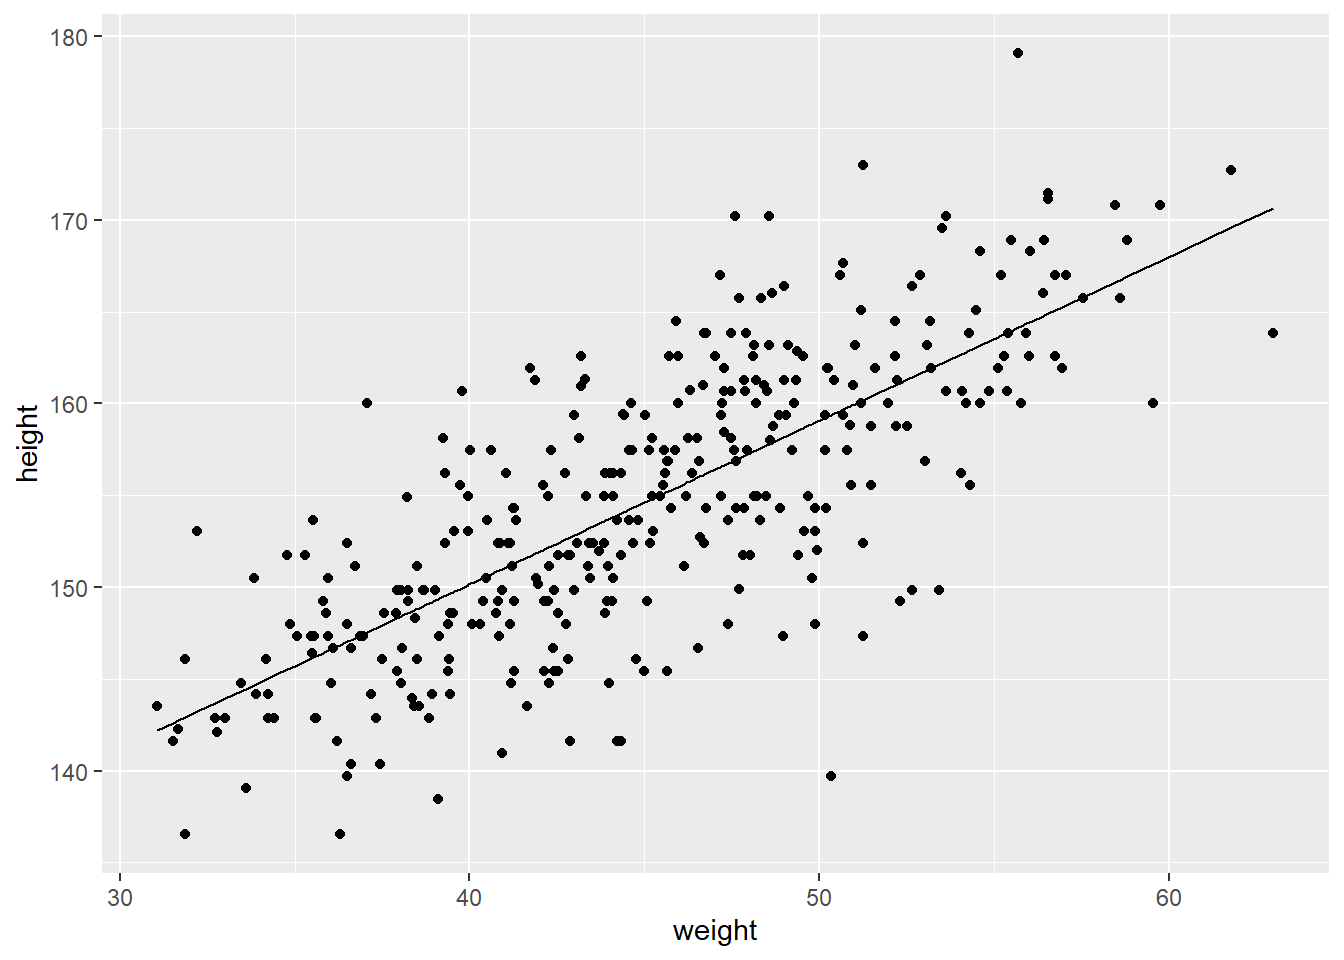
\includegraphics{notes-on-statistical-rethinking_files/figure-latex/4M7-5-1.pdf}

\begin{Shaded}
\begin{Highlighting}[]
\NormalTok{post \textless{}{-}}\StringTok{ }\KeywordTok{extract.samples}\NormalTok{(m4\_3c)}
\NormalTok{a\_map \textless{}{-}}\StringTok{ }\KeywordTok{mean}\NormalTok{(post}\OperatorTok{$}\NormalTok{a)}
\NormalTok{b\_map \textless{}{-}}\StringTok{ }\KeywordTok{mean}\NormalTok{(post}\OperatorTok{$}\NormalTok{b)}

\NormalTok{w \textless{}{-}}\StringTok{ }\NormalTok{d2}\OperatorTok{$}\NormalTok{weight}
\NormalTok{prediction \textless{}{-}}\StringTok{ }\NormalTok{a\_map }\OperatorTok{+}\StringTok{ }\NormalTok{b\_map}\OperatorTok{*}\NormalTok{(w }\OperatorTok{{-}}\StringTok{ }\NormalTok{xbar)}

\KeywordTok{ggplot}\NormalTok{(}\DataTypeTok{data =}\NormalTok{ d2, }\KeywordTok{aes}\NormalTok{(}\DataTypeTok{x=}\NormalTok{weight, }\DataTypeTok{y=}\NormalTok{height)) }\OperatorTok{+}\StringTok{ }
\StringTok{  }\KeywordTok{geom\_point}\NormalTok{() }\OperatorTok{+}
\StringTok{  }\KeywordTok{geom\_line}\NormalTok{(}\DataTypeTok{data =} \OtherTok{NULL}\NormalTok{, }\KeywordTok{aes}\NormalTok{(}\DataTypeTok{x=}\NormalTok{w, }\DataTypeTok{y=}\NormalTok{prediction))}
\end{Highlighting}
\end{Shaded}

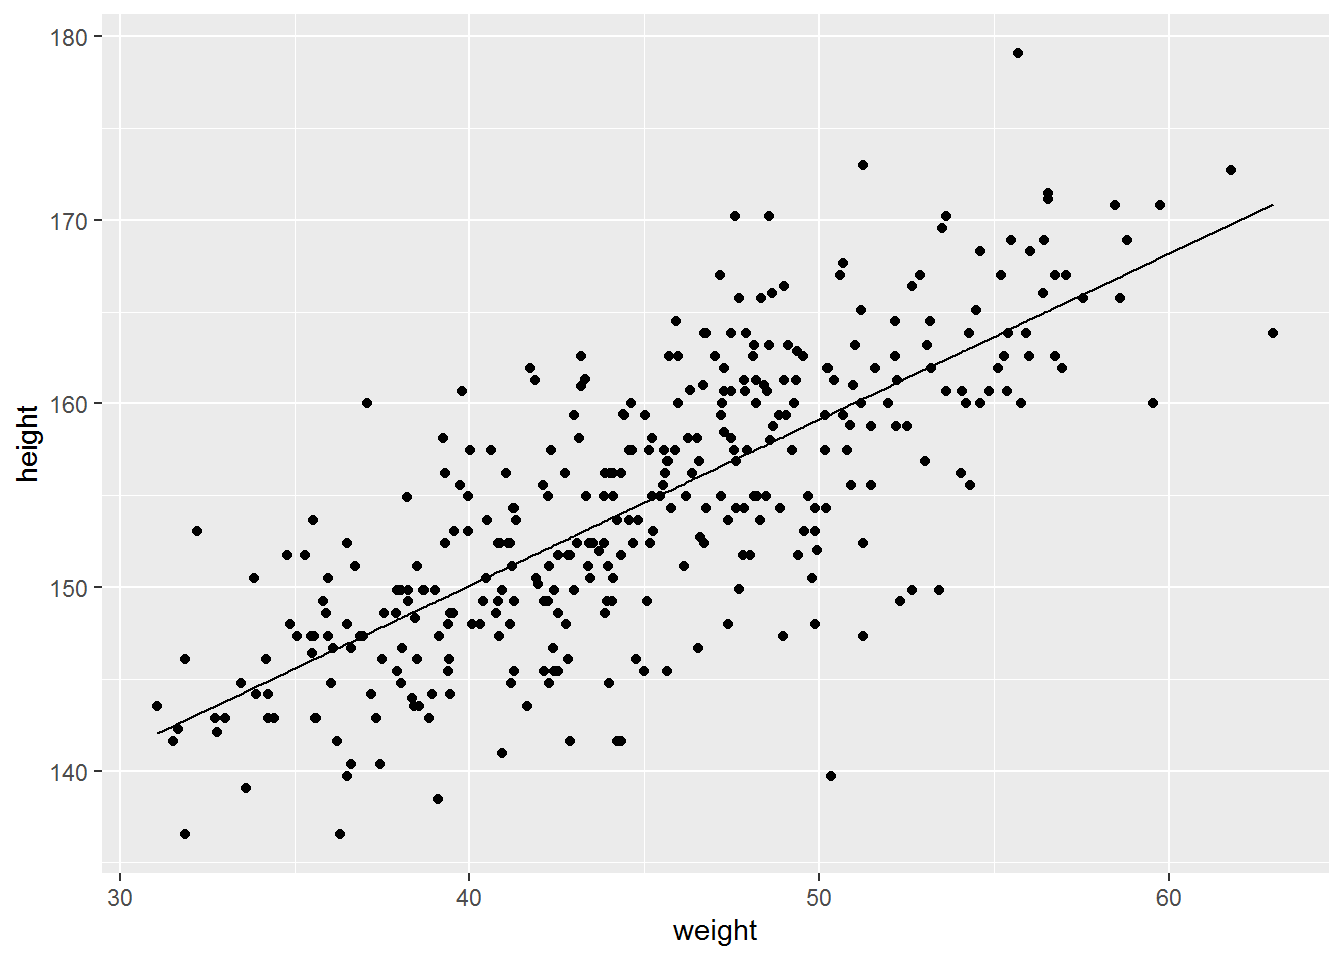
\includegraphics{notes-on-statistical-rethinking_files/figure-latex/unnamed-chunk-14-1.pdf}

\hypertarget{m8}{%
\subsubsection*{4M8}\label{m8}}
\addcontentsline{toc}{subsubsection}{4M8}

In the chapter, we used 15 knots with the cherry blossom spline. Increase the number of knots and observe what happens to the resulting spline. Then adjust also the width of the prior on the weights---change the standard deviation of the prior and watch what happens. What do you think the combination of knot number and the prior on the weights controls?

\begin{Shaded}
\begin{Highlighting}[]
\KeywordTok{data}\NormalTok{(cherry\_blossoms)}
\NormalTok{d \textless{}{-}}\StringTok{ }\NormalTok{cherry\_blossoms}
\NormalTok{d2 \textless{}{-}}\StringTok{ }\NormalTok{d[ }\KeywordTok{complete.cases}\NormalTok{(d}\OperatorTok{$}\NormalTok{doy) , ] }\CommentTok{\# complete cases on doy}
\NormalTok{num\_knots \textless{}{-}}\StringTok{ }\DecValTok{30}
\NormalTok{knot\_list \textless{}{-}}\StringTok{ }\KeywordTok{quantile}\NormalTok{( d2}\OperatorTok{$}\NormalTok{year , }\DataTypeTok{probs=}\KeywordTok{seq}\NormalTok{(}\DecValTok{0}\NormalTok{,}\DecValTok{1}\NormalTok{,}\DataTypeTok{length.out=}\NormalTok{num\_knots) )}
\NormalTok{B \textless{}{-}}\StringTok{ }\KeywordTok{bs}\NormalTok{(d2}\OperatorTok{$}\NormalTok{year,}
        \DataTypeTok{knots=}\NormalTok{knot\_list[}\OperatorTok{{-}}\KeywordTok{c}\NormalTok{(}\DecValTok{1}\NormalTok{,num\_knots)],}
        \DataTypeTok{degree=}\DecValTok{3}\NormalTok{ , }\DataTypeTok{intercept=}\OtherTok{TRUE}\NormalTok{)}

\NormalTok{m4}\FloatTok{.7}\NormalTok{\_}\DecValTok{30}\NormalTok{ \textless{}{-}}\StringTok{ }\KeywordTok{quap}\NormalTok{(}
  \KeywordTok{alist}\NormalTok{(}
\NormalTok{    D }\OperatorTok{\textasciitilde{}}\StringTok{ }\KeywordTok{dnorm}\NormalTok{( mu , sigma ) ,}
\NormalTok{    mu \textless{}{-}}\StringTok{ }\NormalTok{a }\OperatorTok{+}\StringTok{ }\NormalTok{B }\OperatorTok{\%*\%}\StringTok{ }\NormalTok{w ,}
\NormalTok{    a }\OperatorTok{\textasciitilde{}}\StringTok{ }\KeywordTok{dnorm}\NormalTok{(}\DecValTok{100}\NormalTok{,}\DecValTok{10}\NormalTok{),}
\NormalTok{    w }\OperatorTok{\textasciitilde{}}\StringTok{ }\KeywordTok{dnorm}\NormalTok{(}\DecValTok{0}\NormalTok{,}\DecValTok{10}\NormalTok{),}
\NormalTok{    sigma }\OperatorTok{\textasciitilde{}}\StringTok{ }\KeywordTok{dexp}\NormalTok{(}\DecValTok{1}\NormalTok{)), }
  \DataTypeTok{data=}\KeywordTok{list}\NormalTok{(}\DataTypeTok{D=}\NormalTok{d2}\OperatorTok{$}\NormalTok{doy, }\DataTypeTok{B=}\NormalTok{B) ,}
  \DataTypeTok{start=}\KeywordTok{list}\NormalTok{(}\DataTypeTok{w=}\KeywordTok{rep}\NormalTok{(}\DecValTok{0}\NormalTok{, }\KeywordTok{ncol}\NormalTok{(B))))}

\NormalTok{mu \textless{}{-}}\StringTok{ }\KeywordTok{link}\NormalTok{( m4}\FloatTok{.7}\NormalTok{\_}\DecValTok{30}\NormalTok{ )}
\NormalTok{mu\_PI \textless{}{-}}\StringTok{ }\KeywordTok{apply}\NormalTok{(mu,}\DecValTok{2}\NormalTok{, PI, }\FloatTok{0.97}\NormalTok{)}
\KeywordTok{plot}\NormalTok{( d2}\OperatorTok{$}\NormalTok{year , d2}\OperatorTok{$}\NormalTok{doy , }\DataTypeTok{col=}\KeywordTok{col.alpha}\NormalTok{(rangi2,}\FloatTok{0.3}\NormalTok{) , }\DataTypeTok{pch=}\DecValTok{16}\NormalTok{ )}
\KeywordTok{shade}\NormalTok{( mu\_PI , d2}\OperatorTok{$}\NormalTok{year , }\DataTypeTok{col=}\KeywordTok{col.alpha}\NormalTok{(}\StringTok{"black"}\NormalTok{,}\FloatTok{0.5}\NormalTok{) )}
\end{Highlighting}
\end{Shaded}

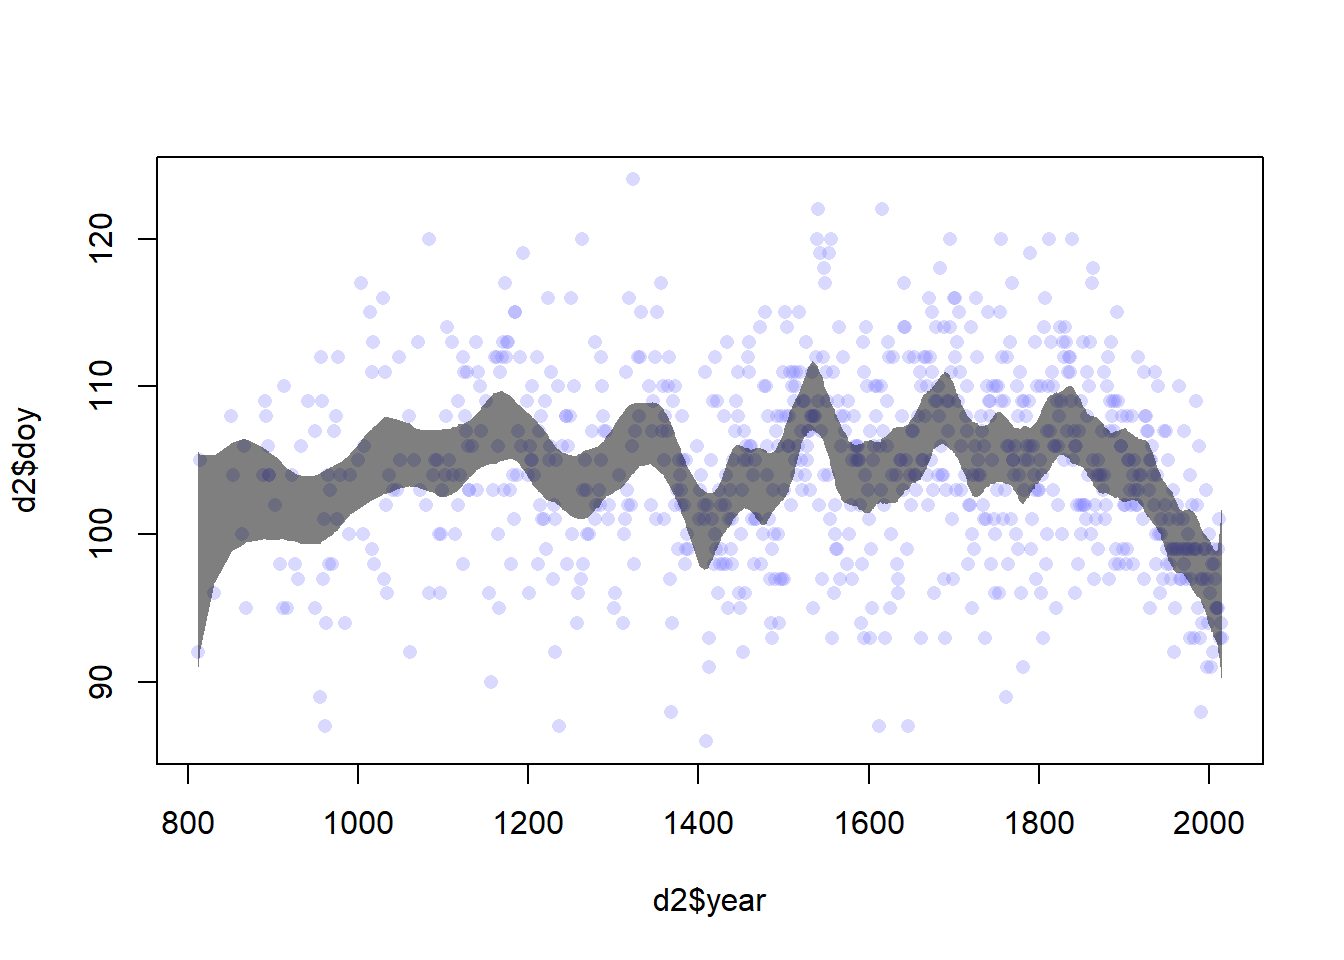
\includegraphics{notes-on-statistical-rethinking_files/figure-latex/4M8-1.pdf}
\textbf{Together, they control just how wiggly vs.~smooth the resultant curve is.}

\hypertarget{h1-2}{%
\subsubsection*{4H1}\label{h1-2}}
\addcontentsline{toc}{subsubsection}{4H1}

The weights listed below were recorded in the !Kung census, but heights were not recorded for these individuals. Provide predicted heights and 89\% intervals for each of these individuals. That is, fill in the table below, using model-based predictions.

\begin{Shaded}
\begin{Highlighting}[]
\NormalTok{predicted\_weight \textless{}{-}}\StringTok{ }
\StringTok{  }\KeywordTok{tibble}\NormalTok{(}\DataTypeTok{Individual =} \DecValTok{1}\OperatorTok{:}\DecValTok{5}\NormalTok{,}
         \DataTypeTok{weight =} \KeywordTok{c}\NormalTok{(}\FloatTok{46.95}\NormalTok{, }\FloatTok{43.72}\NormalTok{, }\FloatTok{64.78}\NormalTok{, }\FloatTok{32.59}\NormalTok{, }\FloatTok{54.63}\NormalTok{))}

\CommentTok{\# getting sampled means}
\NormalTok{posterior\_mu \textless{}{-}}\StringTok{ }\KeywordTok{link}\NormalTok{(m4\_3c, }\DataTypeTok{data=}\NormalTok{predicted\_weight)}

\NormalTok{predicted\_weight \textless{}{-}}\StringTok{ }\NormalTok{predicted\_weight }\OperatorTok{\%\textgreater{}\%}
\StringTok{  }\KeywordTok{mutate}\NormalTok{(}\StringTok{\textasciigrave{}}\DataTypeTok{expected height}\StringTok{\textasciigrave{}}\NormalTok{ =}\StringTok{ }\KeywordTok{apply}\NormalTok{(posterior\_mu, }\DecValTok{2}\NormalTok{, mean), }
         \DataTypeTok{LowerCI =} \KeywordTok{round}\NormalTok{(}\KeywordTok{apply}\NormalTok{(posterior\_mu, }\DecValTok{2}\NormalTok{, quantile, }\DataTypeTok{probs=}\NormalTok{(}\DecValTok{1}\FloatTok{{-}0.89}\NormalTok{)}\OperatorTok{/}\DecValTok{2}\NormalTok{), }\DecValTok{2}\NormalTok{),}
         \DataTypeTok{UpperCI =} \KeywordTok{round}\NormalTok{(}\KeywordTok{apply}\NormalTok{(posterior\_mu, }\DecValTok{2}\NormalTok{, quantile, }\DataTypeTok{probs=}\DecValTok{1}\OperatorTok{{-}}\NormalTok{(}\DecValTok{1}\FloatTok{{-}0.89}\NormalTok{)}\OperatorTok{/}\DecValTok{2}\NormalTok{), }\DecValTok{2}\NormalTok{),}
         \StringTok{\textasciigrave{}}\DataTypeTok{89\% interval}\StringTok{\textasciigrave{}}\NormalTok{ =}\StringTok{ }\NormalTok{glue}\OperatorTok{::}\KeywordTok{glue}\NormalTok{(}\StringTok{"\{LowerCI\}..\{UpperCI\}"}\NormalTok{))  }\OperatorTok{\%\textgreater{}\%}
\StringTok{  }\KeywordTok{select}\NormalTok{(}\OperatorTok{{-}}\NormalTok{LowerCI, }\OperatorTok{{-}}\NormalTok{UpperCI)}

\NormalTok{knitr}\OperatorTok{::}\KeywordTok{kable}\NormalTok{(predicted\_weight)}
\end{Highlighting}
\end{Shaded}

\begin{tabular}{r|r|r|l}
\hline
Individual & weight & expected height & 89\% interval\\
\hline
1 & 46.95 & 156.3876 & 155.97..156.83\\
\hline
2 & 43.72 & 153.4682 & 153.05..153.89\\
\hline
3 & 64.78 & 172.5032 & 171.1..173.91\\
\hline
4 & 32.59 & 143.4083 & 142.5..144.37\\
\hline
5 & 54.63 & 163.3292 & 162.57..164.07\\
\hline
\end{tabular}

\hypertarget{h2-2}{%
\subsubsection*{4H2}\label{h2-2}}
\addcontentsline{toc}{subsubsection}{4H2}

Select out all the rows in the Howell1 data with ages below 18 years of age. If you do it right, you should end up with a new data frame with 192 rows in it.

\begin{enumerate}
\def\labelenumi{\alph{enumi}.}
\tightlist
\item
  Fit a linear regression to these data, using quap. Present and interpret the estimates. For
  every 10 units of increase in weight, how much taller does the model predict a child gets?
\end{enumerate}

\begin{Shaded}
\begin{Highlighting}[]
\NormalTok{kung\_kids \textless{}{-}}\StringTok{ }\KeywordTok{filter}\NormalTok{(Howell1, age }\OperatorTok{\textless{}}\StringTok{ }\DecValTok{18}\NormalTok{)}

\CommentTok{\# define the average weight, x{-}bar}
\NormalTok{avg\_kid\_weight \textless{}{-}}\StringTok{ }\KeywordTok{mean}\NormalTok{(kung\_kids}\OperatorTok{$}\NormalTok{weight)}

\CommentTok{\# fit model}
\NormalTok{kung\_kids\_fit \textless{}{-}}\StringTok{ }\KeywordTok{quap}\NormalTok{(}
  \KeywordTok{alist}\NormalTok{(}
\NormalTok{    height }\OperatorTok{\textasciitilde{}}\StringTok{ }\KeywordTok{dnorm}\NormalTok{(mu, sigma),}
\NormalTok{    mu \textless{}{-}}\StringTok{ }\NormalTok{a }\OperatorTok{+}\StringTok{ }\NormalTok{b }\OperatorTok{*}\StringTok{ }\NormalTok{(weight }\OperatorTok{{-}}\StringTok{ }\NormalTok{avg\_kid\_weight),}
\NormalTok{    a }\OperatorTok{\textasciitilde{}}\StringTok{ }\KeywordTok{dnorm}\NormalTok{(}\DecValTok{140}\NormalTok{, }\DecValTok{20}\NormalTok{) ,}
\NormalTok{    b }\OperatorTok{\textasciitilde{}}\StringTok{ }\KeywordTok{dlnorm}\NormalTok{(}\DecValTok{0}\NormalTok{, }\DecValTok{1}\NormalTok{) ,}
\NormalTok{    sigma }\OperatorTok{\textasciitilde{}}\StringTok{ }\KeywordTok{dunif}\NormalTok{(}\DecValTok{0}\NormalTok{, }\DecValTok{50}\NormalTok{)) , }
  \DataTypeTok{data=}\NormalTok{kung\_kids)}

\KeywordTok{precis}\NormalTok{(kung\_kids\_fit)}
\end{Highlighting}
\end{Shaded}

\begin{verbatim}
##             mean         sd       5.5%      94.5%
## a     108.348193 0.60862837 107.375488 109.320899
## b       2.716657 0.06831574   2.607475   2.825839
## sigma   8.437208 0.43057023   7.749073   9.125342
\end{verbatim}

\begin{Shaded}
\begin{Highlighting}[]
\NormalTok{b\_mean \textless{}{-}}\StringTok{ }\KeywordTok{precis}\NormalTok{(kung\_kids\_fit)[}\StringTok{\textquotesingle{}b\textquotesingle{}}\NormalTok{, }\StringTok{\textquotesingle{}mean\textquotesingle{}}\NormalTok{]}
\end{Highlighting}
\end{Shaded}

\textbf{For every 10 units of increase in weight, the model predict a child will get 27.2 cm taller.}

\begin{enumerate}
\def\labelenumi{\alph{enumi}.}
\setcounter{enumi}{1}
\tightlist
\item
  Plot the raw data, with height on the vertical axis and weight on the horizontal axis. Superimpose the MAP regression line and 89\% interval for the mean. Also superimpose the 89\% interval for predicted heights.
\end{enumerate}

\begin{Shaded}
\begin{Highlighting}[]
\NormalTok{mean\_estimates \textless{}{-}}\StringTok{ }\KeywordTok{tibble}\NormalTok{(}\DataTypeTok{weight =} \KeywordTok{seq}\NormalTok{(}\KeywordTok{min}\NormalTok{(kung\_kids}\OperatorTok{$}\NormalTok{weight), }\KeywordTok{max}\NormalTok{(kung\_kids}\OperatorTok{$}\NormalTok{weight), }\DataTypeTok{length.out =} \DecValTok{100}\NormalTok{))}
\NormalTok{sample\_means \textless{}{-}}\StringTok{ }\KeywordTok{link}\NormalTok{(kung\_kids\_fit, mean\_estimates)}
\NormalTok{mean\_estimates \textless{}{-}}
\StringTok{  }\NormalTok{mean\_estimates }\OperatorTok{\%\textgreater{}\%}
\StringTok{  }\KeywordTok{mutate}\NormalTok{(}\DataTypeTok{mu =} \KeywordTok{apply}\NormalTok{(sample\_means, }\DecValTok{2}\NormalTok{, mean),}
         \DataTypeTok{lowerCI =} \KeywordTok{apply}\NormalTok{(sample\_means, }\DecValTok{2}\NormalTok{, quantile, }\DataTypeTok{probs=}\NormalTok{(}\DecValTok{1}\FloatTok{{-}0.89}\NormalTok{)}\OperatorTok{/}\DecValTok{2}\NormalTok{),}
         \DataTypeTok{upperCI =} \KeywordTok{apply}\NormalTok{(sample\_means, }\DecValTok{2}\NormalTok{, quantile, }\DataTypeTok{probs=}\DecValTok{1}\OperatorTok{{-}}\NormalTok{(}\DecValTok{1}\FloatTok{{-}0.89}\NormalTok{)}\OperatorTok{/}\DecValTok{2}\NormalTok{))}

\NormalTok{simulated\_height\_samples \textless{}{-}}\StringTok{ }\KeywordTok{sim}\NormalTok{(kung\_kids\_fit, mean\_estimates)}
\NormalTok{simulated\_height \textless{}{-}}
\StringTok{  }\NormalTok{mean\_estimates }\OperatorTok{\%\textgreater{}\%}
\StringTok{  }\KeywordTok{mutate}\NormalTok{(}\DataTypeTok{lowerCI =} \KeywordTok{apply}\NormalTok{(simulated\_height\_samples, }\DecValTok{2}\NormalTok{, quantile, }\DataTypeTok{probs=}\NormalTok{(}\DecValTok{1}\FloatTok{{-}0.89}\NormalTok{)}\OperatorTok{/}\DecValTok{2}\NormalTok{),}
         \DataTypeTok{upperCI =} \KeywordTok{apply}\NormalTok{(simulated\_height\_samples, }\DecValTok{2}\NormalTok{, quantile, }\DataTypeTok{probs=}\DecValTok{1}\OperatorTok{{-}}\NormalTok{(}\DecValTok{1}\FloatTok{{-}0.89}\NormalTok{)}\OperatorTok{/}\DecValTok{2}\NormalTok{))}


\KeywordTok{ggplot}\NormalTok{(}\DataTypeTok{data =}\NormalTok{ kung\_kids, }\KeywordTok{aes}\NormalTok{(}\DataTypeTok{x =}\NormalTok{ weight, }\DataTypeTok{y=}\NormalTok{height)) }\OperatorTok{+}\StringTok{ }
\StringTok{  }\KeywordTok{geom\_ribbon}\NormalTok{(}\DataTypeTok{data=}\NormalTok{simulated\_height, }\KeywordTok{aes}\NormalTok{(}\DataTypeTok{y=}\NormalTok{lowerCI, }\DataTypeTok{ymin=}\NormalTok{lowerCI, }\DataTypeTok{ymax=}\NormalTok{upperCI), }\DataTypeTok{fill=}\StringTok{"blue"}\NormalTok{, }\DataTypeTok{alpha=}\FloatTok{0.5}\NormalTok{)}\OperatorTok{+}
\StringTok{  }\KeywordTok{geom\_ribbon}\NormalTok{(}\DataTypeTok{data=}\NormalTok{mean\_estimates, }\KeywordTok{aes}\NormalTok{(}\DataTypeTok{y=}\NormalTok{mu, }\DataTypeTok{ymin=}\NormalTok{lowerCI, }\DataTypeTok{ymax=}\NormalTok{upperCI), }\DataTypeTok{fill=}\StringTok{"blue"}\NormalTok{)}\OperatorTok{+}
\StringTok{  }\KeywordTok{geom\_point}\NormalTok{() }\OperatorTok{+}\StringTok{ }
\StringTok{  }\KeywordTok{geom\_line}\NormalTok{(}\DataTypeTok{data=}\NormalTok{mean\_estimates, }\KeywordTok{aes}\NormalTok{(}\DataTypeTok{y=}\NormalTok{mu))}
\end{Highlighting}
\end{Shaded}

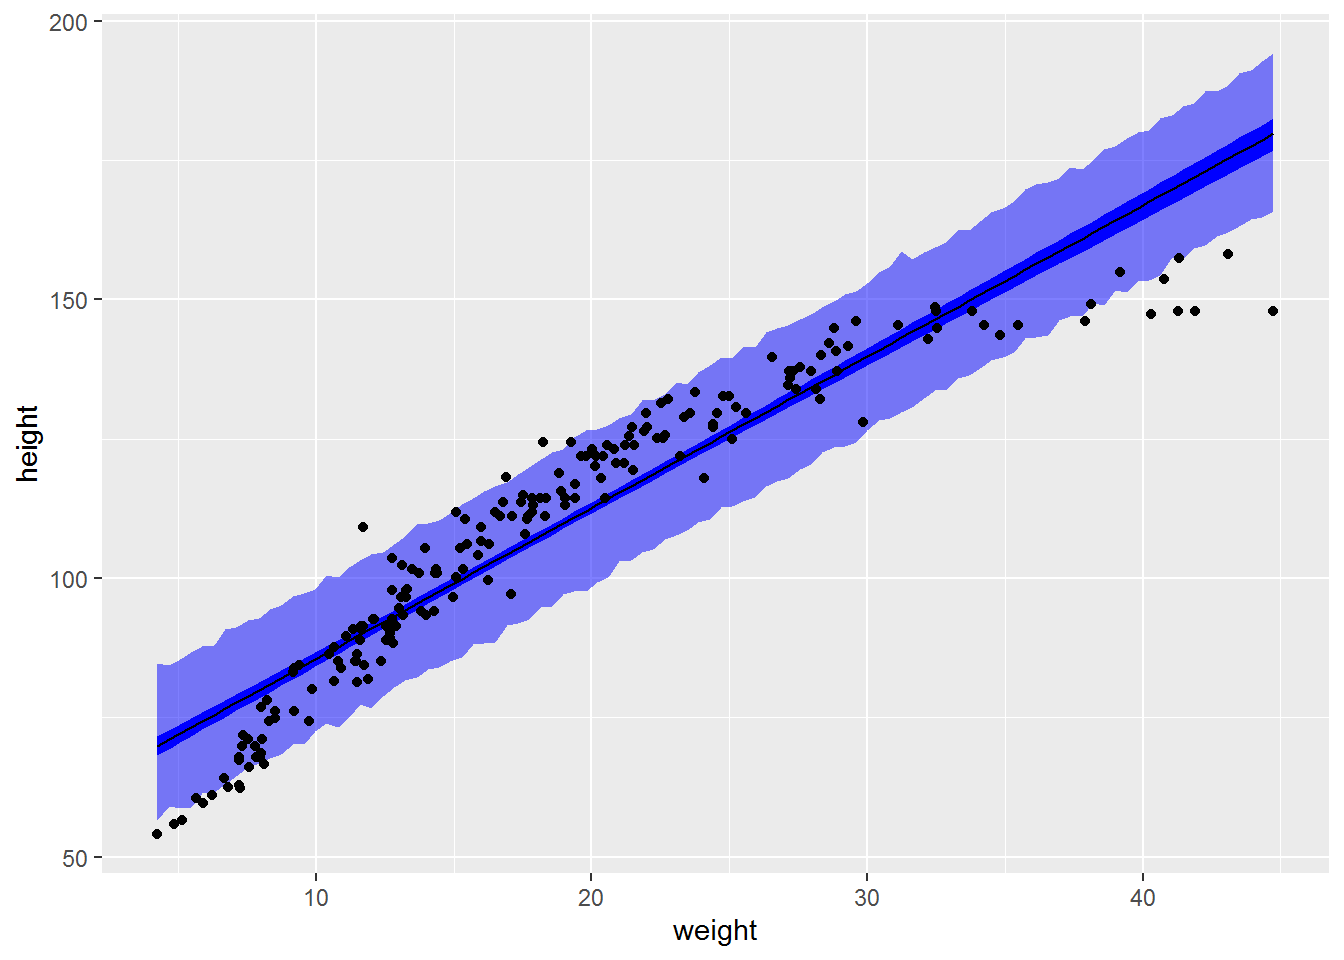
\includegraphics{notes-on-statistical-rethinking_files/figure-latex/4H2b-1.pdf}

\begin{enumerate}
\def\labelenumi{\alph{enumi}.}
\setcounter{enumi}{2}
\tightlist
\item
  What aspects of the model fit concern you? Describe the kinds of assumptions you would
  change, if any, to improve the model. You don't have to write any new code. Just explain what the
  model appears to be doing a bad job of, and what you hypothesize would be a better model.
\end{enumerate}

\textbf{The relationship is clearly no linear with rapid growth for smaller children turning into a more slow one for older ones.}

\hypertarget{h3-2}{%
\subsubsection*{4H3}\label{h3-2}}
\addcontentsline{toc}{subsubsection}{4H3}

Suppose a colleague of yours, who works on allometry, glances at the practice problems just above. Your colleague exclaims, ``That's silly. Everyone knows that it's only the logarithm of body weight that scales with height!'' Let's take your colleague's advice and see what happens.

\begin{enumerate}
\def\labelenumi{(\alph{enumi})}
\tightlist
\item
  Model the relationship between height (cm) and the natural logarithm of weight (log-kg). Use the entire Howell1 data frame, all 544 rows, adults and non-adults. Can you interpret the resulting estimates?
\end{enumerate}

\begin{Shaded}
\begin{Highlighting}[]
\NormalTok{kung \textless{}{-}}\StringTok{ }
\StringTok{  }\NormalTok{Howell1 }\OperatorTok{\%\textgreater{}\%}
\StringTok{  }\KeywordTok{mutate}\NormalTok{(}\DataTypeTok{logWeight =} \KeywordTok{log}\NormalTok{(weight))}

\CommentTok{\# define the average weight, x{-}bar}
\NormalTok{avg\_log\_weight \textless{}{-}}\StringTok{ }\KeywordTok{mean}\NormalTok{(kung}\OperatorTok{$}\NormalTok{logWeight)}

\CommentTok{\# fit model}
\NormalTok{kung\_fit \textless{}{-}}\StringTok{ }\KeywordTok{quap}\NormalTok{(}
  \KeywordTok{alist}\NormalTok{(}
\NormalTok{    height }\OperatorTok{\textasciitilde{}}\StringTok{ }\KeywordTok{dnorm}\NormalTok{(mu, sigma),}
\NormalTok{    mu \textless{}{-}}\StringTok{ }\NormalTok{a }\OperatorTok{+}\StringTok{ }\NormalTok{b }\OperatorTok{*}\StringTok{ }\NormalTok{(logWeight }\OperatorTok{{-}}\StringTok{ }\NormalTok{avg\_log\_weight),}
\NormalTok{    a }\OperatorTok{\textasciitilde{}}\StringTok{ }\KeywordTok{dnorm}\NormalTok{(}\DecValTok{140}\NormalTok{, }\DecValTok{20}\NormalTok{) ,}
\NormalTok{    b }\OperatorTok{\textasciitilde{}}\StringTok{ }\KeywordTok{dlnorm}\NormalTok{(}\DecValTok{0}\NormalTok{, }\DecValTok{1}\NormalTok{) ,}
\NormalTok{    sigma }\OperatorTok{\textasciitilde{}}\StringTok{ }\KeywordTok{dunif}\NormalTok{(}\DecValTok{0}\NormalTok{, }\DecValTok{50}\NormalTok{)) , }
  \DataTypeTok{data=}\NormalTok{kung)}

\KeywordTok{precis}\NormalTok{(kung\_fit)}
\end{Highlighting}
\end{Shaded}

\begin{verbatim}
##             mean        sd       5.5%      94.5%
## a     138.263717 0.2201177 137.911927 138.615508
## b      47.072415 0.3826000  46.460947  47.683884
## sigma   5.134294 0.1556374   4.885555   5.383032
\end{verbatim}

\textbf{Not really, as \texttt{b} now refers to change in height in response to 1 log-Kg of weight.}

\begin{enumerate}
\def\labelenumi{(\alph{enumi})}
\setcounter{enumi}{1}
\tightlist
\item
  Begin with this plot: plot( height \textasciitilde{} weight , data=Howell1 ). Then use samples from the quadratic approximate posterior of the model in (a) to superimpose on the plot:

  \begin{enumerate}
  \def\labelenumii{(\arabic{enumii})}
  \tightlist
  \item
    the predicted mean height as a function of weight,
  \item
    the 97\% interval for the mean, and
  \item
    the 97\% interval for predicted heights.
  \end{enumerate}
\end{enumerate}

\begin{Shaded}
\begin{Highlighting}[]
\NormalTok{mean\_estimates \textless{}{-}}\StringTok{ }
\StringTok{  }\KeywordTok{tibble}\NormalTok{(}\DataTypeTok{weight =} \KeywordTok{seq}\NormalTok{(}\KeywordTok{min}\NormalTok{(kung}\OperatorTok{$}\NormalTok{weight), }\KeywordTok{max}\NormalTok{(kung}\OperatorTok{$}\NormalTok{weight), }\DataTypeTok{length.out =} \DecValTok{100}\NormalTok{)) }\OperatorTok{\%\textgreater{}\%}
\StringTok{  }\KeywordTok{mutate}\NormalTok{(}\DataTypeTok{logWeight =} \KeywordTok{log}\NormalTok{(weight))}

\NormalTok{sample\_means \textless{}{-}}\StringTok{ }\KeywordTok{link}\NormalTok{(kung\_fit, mean\_estimates)}
\NormalTok{mean\_estimates \textless{}{-}}
\StringTok{  }\NormalTok{mean\_estimates }\OperatorTok{\%\textgreater{}\%}
\StringTok{  }\KeywordTok{mutate}\NormalTok{(}\DataTypeTok{mu =} \KeywordTok{apply}\NormalTok{(sample\_means, }\DecValTok{2}\NormalTok{, mean),}
         \DataTypeTok{lowerCI =} \KeywordTok{apply}\NormalTok{(sample\_means, }\DecValTok{2}\NormalTok{, quantile, }\DataTypeTok{probs=}\NormalTok{(}\DecValTok{1}\FloatTok{{-}0.89}\NormalTok{)}\OperatorTok{/}\DecValTok{2}\NormalTok{),}
         \DataTypeTok{upperCI =} \KeywordTok{apply}\NormalTok{(sample\_means, }\DecValTok{2}\NormalTok{, quantile, }\DataTypeTok{probs=}\DecValTok{1}\OperatorTok{{-}}\NormalTok{(}\DecValTok{1}\FloatTok{{-}0.89}\NormalTok{)}\OperatorTok{/}\DecValTok{2}\NormalTok{))}

\NormalTok{simulated\_height\_samples \textless{}{-}}\StringTok{ }\KeywordTok{sim}\NormalTok{(kung\_fit, mean\_estimates)}
\NormalTok{simulated\_height \textless{}{-}}
\StringTok{  }\NormalTok{mean\_estimates }\OperatorTok{\%\textgreater{}\%}
\StringTok{  }\KeywordTok{mutate}\NormalTok{(}\DataTypeTok{lowerCI =} \KeywordTok{apply}\NormalTok{(simulated\_height\_samples, }\DecValTok{2}\NormalTok{, quantile, }\DataTypeTok{probs=}\NormalTok{(}\DecValTok{1}\FloatTok{{-}0.89}\NormalTok{)}\OperatorTok{/}\DecValTok{2}\NormalTok{),}
         \DataTypeTok{upperCI =} \KeywordTok{apply}\NormalTok{(simulated\_height\_samples, }\DecValTok{2}\NormalTok{, quantile, }\DataTypeTok{probs=}\DecValTok{1}\OperatorTok{{-}}\NormalTok{(}\DecValTok{1}\FloatTok{{-}0.89}\NormalTok{)}\OperatorTok{/}\DecValTok{2}\NormalTok{))}


\KeywordTok{ggplot}\NormalTok{(}\DataTypeTok{data =}\NormalTok{ kung, }\KeywordTok{aes}\NormalTok{(}\DataTypeTok{x =}\NormalTok{ weight, }\DataTypeTok{y=}\NormalTok{height)) }\OperatorTok{+}\StringTok{ }
\StringTok{  }\KeywordTok{geom\_ribbon}\NormalTok{(}\DataTypeTok{data=}\NormalTok{simulated\_height, }\KeywordTok{aes}\NormalTok{(}\DataTypeTok{y=}\NormalTok{lowerCI, }\DataTypeTok{ymin=}\NormalTok{lowerCI, }\DataTypeTok{ymax=}\NormalTok{upperCI), }\DataTypeTok{fill=}\StringTok{"blue"}\NormalTok{, }\DataTypeTok{alpha=}\FloatTok{0.5}\NormalTok{)}\OperatorTok{+}
\StringTok{  }\KeywordTok{geom\_ribbon}\NormalTok{(}\DataTypeTok{data=}\NormalTok{mean\_estimates, }\KeywordTok{aes}\NormalTok{(}\DataTypeTok{y=}\NormalTok{mu, }\DataTypeTok{ymin=}\NormalTok{lowerCI, }\DataTypeTok{ymax=}\NormalTok{upperCI), }\DataTypeTok{fill=}\StringTok{"blue"}\NormalTok{)}\OperatorTok{+}
\StringTok{  }\KeywordTok{geom\_point}\NormalTok{() }\OperatorTok{+}\StringTok{ }
\StringTok{  }\KeywordTok{geom\_line}\NormalTok{(}\DataTypeTok{data=}\NormalTok{mean\_estimates, }\KeywordTok{aes}\NormalTok{(}\DataTypeTok{y=}\NormalTok{mu))}
\end{Highlighting}
\end{Shaded}

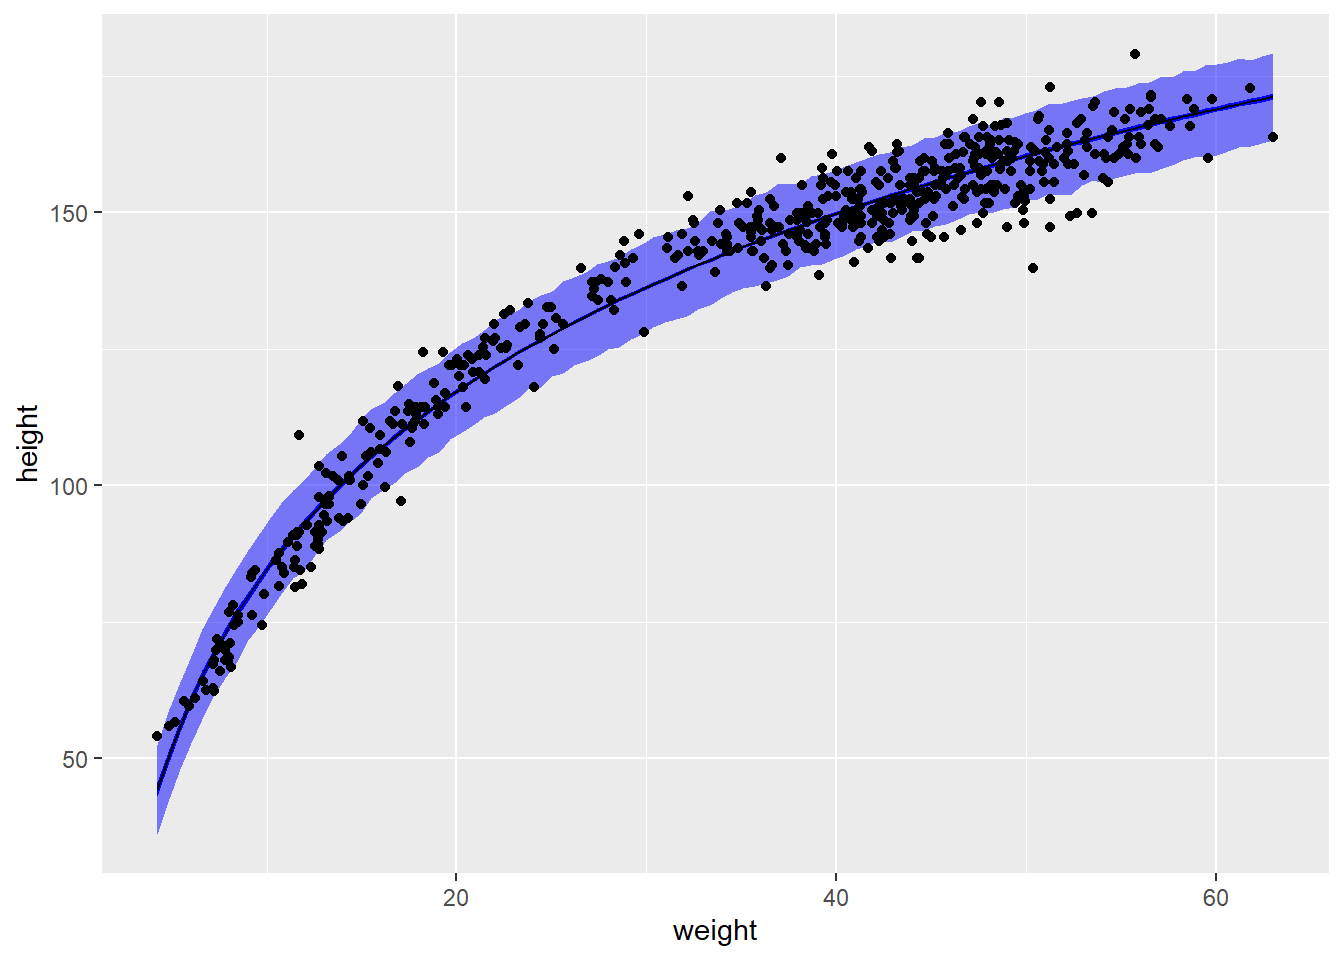
\includegraphics{notes-on-statistical-rethinking_files/figure-latex/4H3b-1.pdf}

\hypertarget{h4-2}{%
\subsubsection*{4H4}\label{h4-2}}
\addcontentsline{toc}{subsubsection}{4H4}

Plot the prior predictive distribution for the parabolic polynomial regression model in the chapter. You can modify the code that plots the linear regression prior predictive distribution. Can you modify the prior distributions of α, β1, and β2 so that the prior predictions stay within the biologically reasonable outcome space? That is to say: Do not try to fit the data by hand. But do try to keep the curves consistent with what you know about height and weight, before seeing these exact data.

\begin{Shaded}
\begin{Highlighting}[]
\NormalTok{zWeight \textless{}{-}}\StringTok{ }\KeywordTok{c}\NormalTok{(}\KeywordTok{scale}\NormalTok{(kung}\OperatorTok{$}\NormalTok{weight))}

\NormalTok{N \textless{}{-}}\StringTok{ }\DecValTok{100}
\NormalTok{a \textless{}{-}}\StringTok{ }\KeywordTok{rnorm}\NormalTok{(N, }\DecValTok{100}\NormalTok{, }\DecValTok{20}\NormalTok{)}
\NormalTok{b1 \textless{}{-}}\StringTok{ }\KeywordTok{rlnorm}\NormalTok{(N, }\FloatTok{2.5}\NormalTok{, }\FloatTok{0.5}\NormalTok{)}
\NormalTok{b2 \textless{}{-}}\StringTok{ }\KeywordTok{rnorm}\NormalTok{(N, }\DecValTok{0}\NormalTok{, }\DecValTok{5}\NormalTok{)}
\NormalTok{x \textless{}{-}}\StringTok{ }\NormalTok{zWeight}
\NormalTok{x2 \textless{}{-}}\StringTok{ }\NormalTok{zWeight}\OperatorTok{\^{}}\DecValTok{2}
\KeywordTok{plot}\NormalTok{(}\OtherTok{NULL}\NormalTok{, }\DataTypeTok{xlim=}\KeywordTok{range}\NormalTok{(zWeight), }\DataTypeTok{ylim=}\KeywordTok{c}\NormalTok{(}\DecValTok{0}\NormalTok{, }\DecValTok{300}\NormalTok{),}
    \DataTypeTok{xlab=}\StringTok{"zWeight"}\NormalTok{, }\DataTypeTok{ylab=}\StringTok{"height"}\NormalTok{)}

\ControlFlowTok{for}\NormalTok{ (i }\ControlFlowTok{in} \DecValTok{1}\OperatorTok{:}\NormalTok{N)\{}
  \KeywordTok{curve}\NormalTok{( a[i] }\OperatorTok{+}\StringTok{ }\NormalTok{b1[i]}\OperatorTok{*}\NormalTok{x }\OperatorTok{+}\StringTok{ }\NormalTok{b2[i]}\OperatorTok{*}\NormalTok{(x}\OperatorTok{*}\NormalTok{x),}
  \DataTypeTok{from=}\KeywordTok{min}\NormalTok{(zWeight), }\DataTypeTok{to=}\KeywordTok{max}\NormalTok{(zWeight), }
  \DataTypeTok{add=}\OtherTok{TRUE}\NormalTok{,}
  \DataTypeTok{col=}\KeywordTok{col.alpha}\NormalTok{(}\StringTok{"black"}\NormalTok{,}\FloatTok{0.2}\NormalTok{))}
\NormalTok{\} }
\end{Highlighting}
\end{Shaded}

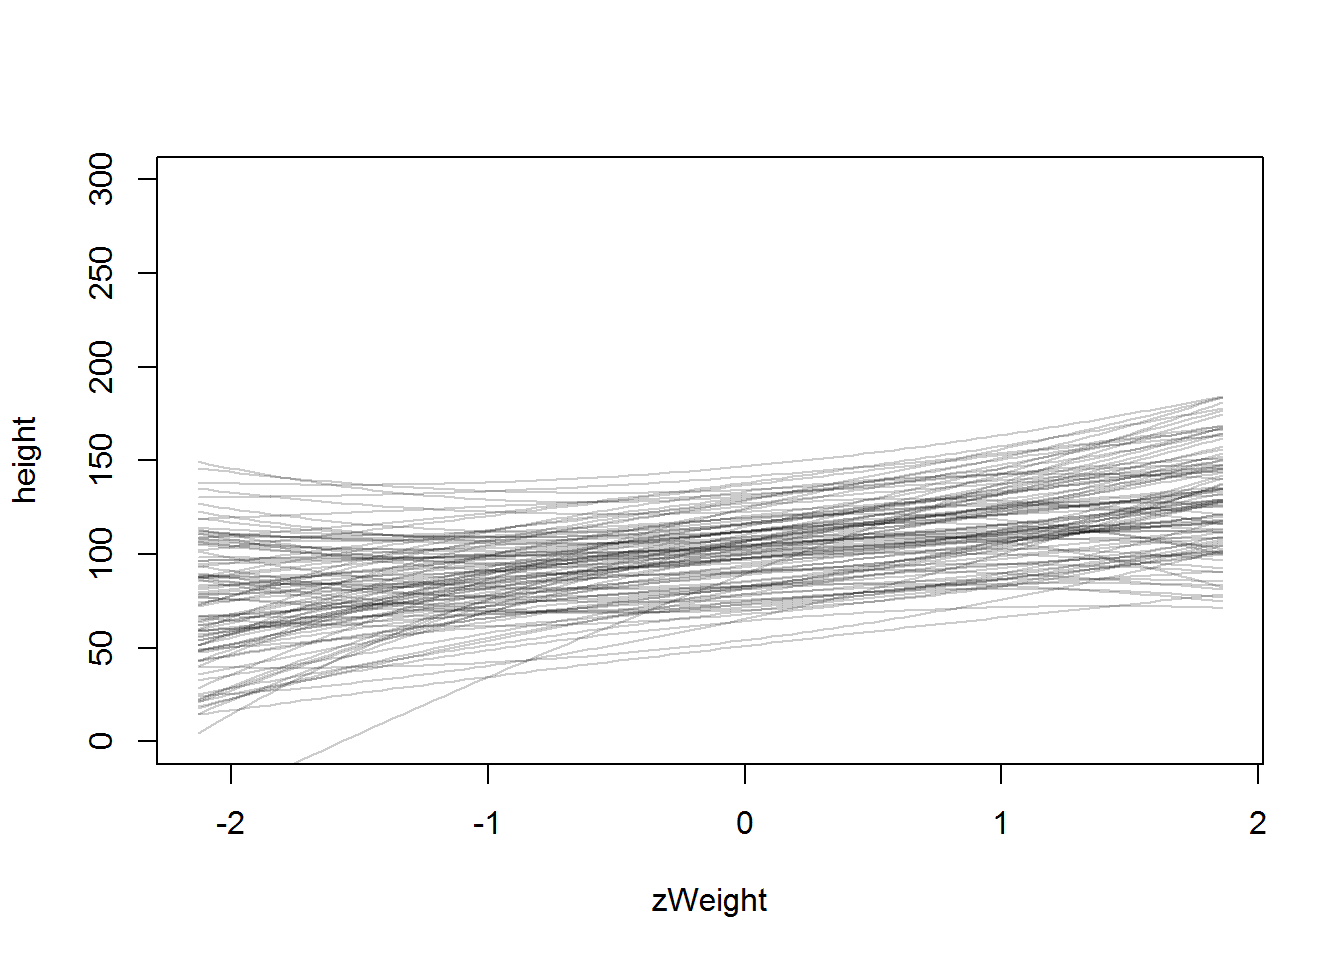
\includegraphics{notes-on-statistical-rethinking_files/figure-latex/4H4-1.pdf}

\hypertarget{h5-1}{%
\subsubsection*{4H5}\label{h5-1}}
\addcontentsline{toc}{subsubsection}{4H5}

Return to data(cherry\_blossoms) and model the association between blossom date (doy) and March temperature (temp). Note that there are many missing values in both variables. You may consider a linear model, a polynomial, or a spline on temperature. How well does temperature trend predict the blossom trend?

\begin{Shaded}
\begin{Highlighting}[]
\NormalTok{sakura \textless{}{-}}\StringTok{ }
\StringTok{  }\NormalTok{cherry\_blossoms }\OperatorTok{\%\textgreater{}\%}
\StringTok{  }\KeywordTok{drop\_na}\NormalTok{(doy, temp)}

\NormalTok{avg\_temp \textless{}{-}}\StringTok{ }\KeywordTok{mean}\NormalTok{(sakura}\OperatorTok{$}\NormalTok{temp)}

\NormalTok{sakura\_fit \textless{}{-}}\StringTok{ }\KeywordTok{quap}\NormalTok{(}
  \KeywordTok{alist}\NormalTok{(}
\NormalTok{    doy }\OperatorTok{\textasciitilde{}}\StringTok{ }\KeywordTok{dnorm}\NormalTok{(mu, sigma),}
\NormalTok{    mu \textless{}{-}}\StringTok{ }\NormalTok{a }\OperatorTok{+}\StringTok{ }\NormalTok{b }\OperatorTok{*}\StringTok{ }\NormalTok{(temp }\OperatorTok{{-}}\StringTok{ }\NormalTok{avg\_temp),}
\NormalTok{    a }\OperatorTok{\textasciitilde{}}\StringTok{ }\KeywordTok{dnorm}\NormalTok{(}\DecValTok{75}\NormalTok{, }\DecValTok{30}\NormalTok{), }\CommentTok{\# jan{-}may is about 150 days, so 75±60 is very conservative spring estimate}
\NormalTok{    b }\OperatorTok{\textasciitilde{}}\StringTok{ }\KeywordTok{dnorm}\NormalTok{(}\DecValTok{0}\NormalTok{, }\DecValTok{1}\NormalTok{), }\CommentTok{\# we would assume the relationship to be negative, so higher tempratures leading to sooner blooming}
\NormalTok{    sigma }\OperatorTok{\textasciitilde{}}\StringTok{ }\KeywordTok{dunif}\NormalTok{(}\DecValTok{0}\NormalTok{, }\DecValTok{15}\NormalTok{)), }\CommentTok{\# ±30 gives us a month}
  \DataTypeTok{data=}\NormalTok{sakura)}

\KeywordTok{precis}\NormalTok{(sakura\_fit)}
\end{Highlighting}
\end{Shaded}

\begin{verbatim}
##             mean        sd       5.5%      94.5%
## a     104.919743 0.2107589 104.582909 105.256576
## b      -2.733661 0.2951189  -3.205318  -2.262004
## sigma   5.912675 0.1491559   5.674295   6.151055
\end{verbatim}

\begin{Shaded}
\begin{Highlighting}[]
\NormalTok{mean\_estimates \textless{}{-}}\StringTok{ }
\StringTok{  }\KeywordTok{tibble}\NormalTok{(}\DataTypeTok{temp =} \KeywordTok{seq}\NormalTok{(}\KeywordTok{min}\NormalTok{(sakura}\OperatorTok{$}\NormalTok{temp), }\KeywordTok{max}\NormalTok{(sakura}\OperatorTok{$}\NormalTok{temp), }\DataTypeTok{length.out =} \DecValTok{100}\NormalTok{))}

\NormalTok{sample\_means \textless{}{-}}\StringTok{ }\KeywordTok{link}\NormalTok{(sakura\_fit, mean\_estimates)}
\NormalTok{mean\_estimates \textless{}{-}}
\StringTok{  }\NormalTok{mean\_estimates }\OperatorTok{\%\textgreater{}\%}
\StringTok{  }\KeywordTok{mutate}\NormalTok{(}\DataTypeTok{mu =} \KeywordTok{apply}\NormalTok{(sample\_means, }\DecValTok{2}\NormalTok{, mean),}
         \DataTypeTok{lowerCI =} \KeywordTok{apply}\NormalTok{(sample\_means, }\DecValTok{2}\NormalTok{, quantile, }\DataTypeTok{probs=}\NormalTok{(}\DecValTok{1}\FloatTok{{-}0.89}\NormalTok{)}\OperatorTok{/}\DecValTok{2}\NormalTok{),}
         \DataTypeTok{upperCI =} \KeywordTok{apply}\NormalTok{(sample\_means, }\DecValTok{2}\NormalTok{, quantile, }\DataTypeTok{probs=}\DecValTok{1}\OperatorTok{{-}}\NormalTok{(}\DecValTok{1}\FloatTok{{-}0.89}\NormalTok{)}\OperatorTok{/}\DecValTok{2}\NormalTok{))}

\NormalTok{simulated\_doy\_samples \textless{}{-}}\StringTok{ }\KeywordTok{sim}\NormalTok{(sakura\_fit, mean\_estimates)}
\NormalTok{simulated\_doy \textless{}{-}}
\StringTok{  }\NormalTok{mean\_estimates }\OperatorTok{\%\textgreater{}\%}
\StringTok{  }\KeywordTok{mutate}\NormalTok{(}\DataTypeTok{lowerCI =} \KeywordTok{apply}\NormalTok{(simulated\_doy\_samples, }\DecValTok{2}\NormalTok{, quantile, }\DataTypeTok{probs=}\NormalTok{(}\DecValTok{1}\FloatTok{{-}0.89}\NormalTok{)}\OperatorTok{/}\DecValTok{2}\NormalTok{),}
         \DataTypeTok{upperCI =} \KeywordTok{apply}\NormalTok{(simulated\_doy\_samples, }\DecValTok{2}\NormalTok{, quantile, }\DataTypeTok{probs=}\DecValTok{1}\OperatorTok{{-}}\NormalTok{(}\DecValTok{1}\FloatTok{{-}0.89}\NormalTok{)}\OperatorTok{/}\DecValTok{2}\NormalTok{))}

\KeywordTok{ggplot}\NormalTok{(sakura, }\KeywordTok{aes}\NormalTok{(}\DataTypeTok{x =}\NormalTok{ temp, }\DataTypeTok{y=}\NormalTok{doy)) }\OperatorTok{+}\StringTok{ }
\StringTok{  }\KeywordTok{geom\_ribbon}\NormalTok{(}\DataTypeTok{data=}\NormalTok{simulated\_doy, }\KeywordTok{aes}\NormalTok{(}\DataTypeTok{y=}\NormalTok{lowerCI, }\DataTypeTok{ymin=}\NormalTok{lowerCI, }\DataTypeTok{ymax=}\NormalTok{upperCI), }\DataTypeTok{fill=}\StringTok{"blue"}\NormalTok{, }\DataTypeTok{alpha=}\FloatTok{0.5}\NormalTok{)}\OperatorTok{+}
\StringTok{  }\KeywordTok{geom\_ribbon}\NormalTok{(}\DataTypeTok{data=}\NormalTok{mean\_estimates, }\KeywordTok{aes}\NormalTok{(}\DataTypeTok{y=}\NormalTok{mu, }\DataTypeTok{ymin=}\NormalTok{lowerCI, }\DataTypeTok{ymax=}\NormalTok{upperCI), }\DataTypeTok{fill=}\StringTok{"blue"}\NormalTok{)}\OperatorTok{+}
\StringTok{  }\KeywordTok{geom\_point}\NormalTok{() }\OperatorTok{+}\StringTok{ }
\StringTok{  }\KeywordTok{geom\_line}\NormalTok{(}\DataTypeTok{data=}\NormalTok{mean\_estimates, }\KeywordTok{aes}\NormalTok{(}\DataTypeTok{y=}\NormalTok{mu))}
\end{Highlighting}
\end{Shaded}

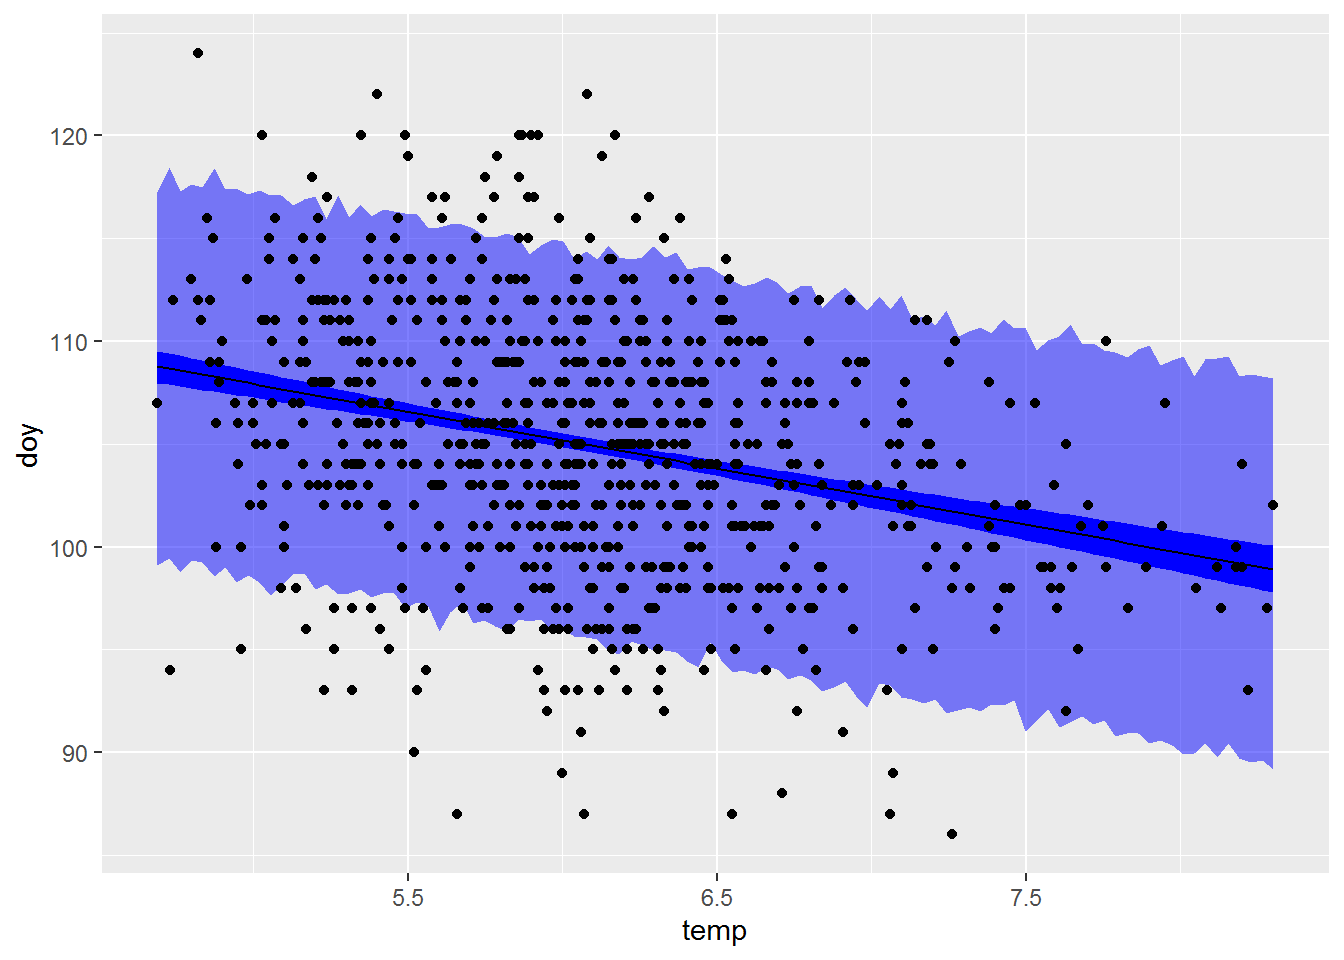
\includegraphics{notes-on-statistical-rethinking_files/figure-latex/4H5-1.pdf}
\textbf{Reasonably well, but you can see a lot of spread in the middle, so other factors are clearly at play.}

\hypertarget{h6}{%
\subsubsection*{4H6}\label{h6}}
\addcontentsline{toc}{subsubsection}{4H6}

Simulate the prior predictive distribution for the cherry blossom spline in the chapter. Adjust the prior on the weights and observe what happens. What do you think the prior on the weights is doing?

\hypertarget{h8}{%
\subsubsection*{4H8}\label{h8}}
\addcontentsline{toc}{subsubsection}{4H8}

The cherry blossom spline in the chapter used an intercept α, but technically it doesn't require one. The first basis functions could substitute for the intercept. Try refitting the cherry blossom spline without the intercept. What else about the model do you need to change to make this work?

  \bibliography{book.bib}

\end{document}
